% Options for packages loaded elsewhere
\PassOptionsToPackage{unicode}{hyperref}
\PassOptionsToPackage{hyphens}{url}
\PassOptionsToPackage{dvipsnames,svgnames,x11names}{xcolor}
%
\documentclass[
  letterpaper,
  12pt,
  british]{tufte-book}

\usepackage{amsmath,amssymb}
\usepackage{lmodern}
\usepackage{iftex}
\ifPDFTeX
  \usepackage[T1]{fontenc}
  \usepackage[utf8]{inputenc}
  \usepackage{textcomp} % provide euro and other symbols
\else % if luatex or xetex
  \usepackage{unicode-math}
  \defaultfontfeatures{Scale=MatchLowercase}
  \defaultfontfeatures[\rmfamily]{Ligatures=TeX,Scale=1}
  \setmainfont[]{ETbb}
  \setsansfont[Scale=MatchUppercase]{TeX Gyre Heros}
\fi
% Use upquote if available, for straight quotes in verbatim environments
\IfFileExists{upquote.sty}{\usepackage{upquote}}{}
\IfFileExists{microtype.sty}{% use microtype if available
  \usepackage[]{microtype}
  \UseMicrotypeSet[protrusion]{basicmath} % disable protrusion for tt fonts
}{}
\usepackage{xcolor}
\setlength{\emergencystretch}{3em} % prevent overfull lines
\setcounter{secnumdepth}{-\maxdimen} % remove section numbering
% Make \paragraph and \subparagraph free-standing
\ifx\paragraph\undefined\else
  \let\oldparagraph\paragraph
  \renewcommand{\paragraph}[1]{\oldparagraph{#1}\mbox{}}
\fi
\ifx\subparagraph\undefined\else
  \let\oldsubparagraph\subparagraph
  \renewcommand{\subparagraph}[1]{\oldsubparagraph{#1}\mbox{}}
\fi


\providecommand{\tightlist}{%
  \setlength{\itemsep}{0pt}\setlength{\parskip}{0pt}}\usepackage{longtable,booktabs,array}
\usepackage{calc} % for calculating minipage widths
% Correct order of tables after \paragraph or \subparagraph
\usepackage{etoolbox}
\makeatletter
\patchcmd\longtable{\par}{\if@noskipsec\mbox{}\fi\par}{}{}
\makeatother
% Allow footnotes in longtable head/foot
\IfFileExists{footnotehyper.sty}{\usepackage{footnotehyper}}{\usepackage{footnote}}
\makesavenoteenv{longtable}
\usepackage{graphicx}
\makeatletter
\def\maxwidth{\ifdim\Gin@nat@width>\linewidth\linewidth\else\Gin@nat@width\fi}
\def\maxheight{\ifdim\Gin@nat@height>\textheight\textheight\else\Gin@nat@height\fi}
\makeatother
% Scale images if necessary, so that they will not overflow the page
% margins by default, and it is still possible to overwrite the defaults
% using explicit options in \includegraphics[width, height, ...]{}
\setkeys{Gin}{width=\maxwidth,height=\maxheight,keepaspectratio}
% Set default figure placement to htbp
\makeatletter
\def\fps@figure{htbp}
\makeatother
\newlength{\cslhangindent}
\setlength{\cslhangindent}{1.5em}
\newlength{\csllabelwidth}
\setlength{\csllabelwidth}{3em}
\newlength{\cslentryspacingunit} % times entry-spacing
\setlength{\cslentryspacingunit}{\parskip}
\newenvironment{CSLReferences}[2] % #1 hanging-ident, #2 entry spacing
 {% don't indent paragraphs
  \setlength{\parindent}{0pt}
  % turn on hanging indent if param 1 is 1
  \ifodd #1
  \let\oldpar\par
  \def\par{\hangindent=\cslhangindent\oldpar}
  \fi
  % set entry spacing
  \setlength{\parskip}{#2\cslentryspacingunit}
 }%
 {}
\usepackage{calc}
\newcommand{\CSLBlock}[1]{#1\hfill\break}
\newcommand{\CSLLeftMargin}[1]{\parbox[t]{\csllabelwidth}{#1}}
\newcommand{\CSLRightInline}[1]{\parbox[t]{\linewidth - \csllabelwidth}{#1}\break}
\newcommand{\CSLIndent}[1]{\hspace{\cslhangindent}#1}

% FIX Marginnote duplication
\usepackage{savesym}
\savesymbol{marginfigure}
\savesymbol{marginnote}
\savesymbol{sidenote}

%%%%%%%
%  FIX Makeuppercase error
%  FIX Font clash Math error
%  See https://tex.stackexchange.com/q/202142/157312
% 

\renewcommand{\textls}[2][5]{%
  \begingroup\addfontfeatures{LetterSpace=#1}#2\endgroup
}
\renewcommand{\allcapsspacing}[1]{\textls[15]{#1}}
\renewcommand{\smallcapsspacing}[1]{\textls[10]{#1}}
\renewcommand{\allcaps}[1]{\textls[15]{\MakeTextUppercase{#1}}}
\renewcommand{\smallcaps}[1]{\smallcapsspacing{\scshape\MakeTextLowercase{#1}}}
\renewcommand{\textsc}[1]{\smallcapsspacing{\textsmallcaps{#1}}}

\PassOptionsToPackage{no-math}{fontspec}
% \usepackage[mathlf, minionint,footnotefigures, frenchmath]{MinionPro}
% \setmainfont{$$}
% \setsansfont{TeX Gyre Heros}[Scale=MatchUppercase]

\ExplSyntaxOn
\int_new:N \l_mathcode_minus_int
\int_new:N \l_mathcode_equal_int
\exp_args:Nx \AtBeginDocument {
  \exp_not:n {
    \int_set:Nn \l_mathcode_minus_int { \XeTeXmathcodenum `\- }
    \int_set:Nn \l_mathcode_equal_int { \XeTeXmathcodenum `\= }
  }
  \mathcode \int_eval:n { `\- } = \number \mathcode `\- \scan_stop:
  \mathcode \int_eval:n { `\= } = \number \mathcode `\= \scan_stop:
}
\AtBeginDocument {
  \XeTeXmathcodenum `\- = \l_mathcode_minus_int
  \XeTeXmathcodenum `\= = \l_mathcode_equal_int
}
\ExplSyntaxOff

\usepackage[italic]{mathastext}
% \setromanfont{TeX Gyre Termes}


%%%%%%%


\usepackage{pdfpages}  % for cover page
\graphicspath{{Images/}} % Make Images/ default figure path


\setlength{\parindent}{0pt}%
\setlength{\RaggedRightParindent}{0pt}
\setlength{\JustifyingParindent}{0pt}%
\setlength{\parskip}{\baselineskip}

%%
% Produces a full title page

\renewcommand{\maketitlepage}[0]{%
  \cleardoublepage%
  {%
  \sffamily%
  \begin{fullwidth}%
  \fontsize{12}{14}\selectfont\par\noindent\textcolor{darkgray}{\allcaps{\thanklessauthor}}%
  \vspace{12.5pc}%
  \fontsize{20}{28}\selectfont\par\noindent\textcolor{darkgray}{\allcaps{\thanklesstitle}}%
  \vfill%
  \fontsize{10}{12}\selectfont\par\noindent\allcaps{\thanklesspublisher}%
  \end{fullwidth}%
  }
  \thispagestyle{empty}%
  \clearpage%
}

% DEFINITIONS


% The fancyvrb package lets us customize the formatting of verbatim
% environments.  We use a slightly smaller font.
\usepackage{fancyvrb}
\fvset{fontsize=\normalsize}

%%
% Prints argument within hanging parentheses (i.e., parentheses that take
% up no horizontal space).  Useful in tabular environments.
\newcommand{\hangp}[1]{\makebox[0pt][r]{(}#1\makebox[0pt][l]{)}}

%%
% Prints an asterisk that takes up no horizontal space.
% Useful in tabular environments.
\newcommand{\hangstar}{\makebox[0pt][l]{*}}

%%
% Prints a trailing space in a smart way.
\usepackage{xspace}


% Prints the month name (e.g., January) and the year (e.g., 2008)
\newcommand{\monthyear}{%
  \ifcase\month\or January\or February\or March\or April\or May\or June\or
  July\or August\or September\or October\or November\or
  December\fi\space\number\year
}


% Prints an epigraph and speaker in sans serif, all-caps type.
\newcommand{\epigraph}[2]{%
  \begin{fullwidth}
  \begin{flushright}
  \sffamily\fontsize{8}{10}\selectfont
  \sffamily\footnotesize
  \begin{doublespace}
  \vspace{-8cm}\noindent\allcaps{#1}\\% epigraph
  \noindent\allcaps{#2}\\% author
  \end{doublespace}
  \vspace{5.1cm}
  \end{flushright}
  \end{fullwidth}
  \normalfont
}


\newcommand{\blankpage}{\newpage\hbox{}\thispagestyle{empty}\newpage}


% insert 4cm before quote
\renewenvironment{quote}{
  \list{}{\leftmargin=3.5cm\topsep=0pt}
  \item\relax\small\itshape
}
{\endlist}


%  change chapter formatting
\titlespacing*{\chapter}{0pt}{5cm}{1cm}
% \titlespacing*{\section}{0pt}{.6em}{.3em}
% \titlespacing*{\subsection}{0pt}{.4em}{.2em}

\titlespacing*{\section}{0pt}{0pt}{0pt}
\titlespacing*{\subsection}{0pt}{0pt}{0pt}


%  Change Figure Caption in the Margin size
% \renewenvironment{@tufte@margin@float}[2][-1.2ex]%
%   {\FloatBarrier% process all floats before this point so the figure/table numbers stay in order.
%   \begin{lrbox}{\@tufte@margin@floatbox}%
%   \begin{minipage}{\marginparwidth}%
%     \@tufte@caption@font\footnotesize% <-- Add fontnotesize
%     \def\@captype{#2}%
%     \hbox{}\vspace*{#1}%
%     \@tufte@caption@justification%
%     \@tufte@margin@par%
%     \noindent\normalsize%<-- restored size
%   }
%   {\end{minipage}%
%   \end{lrbox}%
%   \marginpar{\usebox{\@tufte@margin@floatbox}}%
  % }


% \renewcommand\footnotesize{%
%    \@setfontsize\footnotesize\@viiipt{9}%
%    \abovedisplayskip 5\p@ \@plus2\p@ \@minus4\p@
%    \abovedisplayshortskip \z@ \@plus\p@
%    \belowdisplayshortskip 2.8\p@ \@plus\p@ \@minus2\p@
%    \def\@listi{\leftmargin\leftmargini
%                \topsep 2.5\p@ \@plus\p@ \@minus\p@
%                \parsep 2\p@ \@plus\p@ \@minus\p@
%                \itemsep \parsep}%
%    \belowdisplayskip \abovedisplayskip
% }

% % Define Tuftian float styles (with the caption in the margin)
% \newcommand{\floatc@tufteplain}[2]{%
% \begin{lrbox}{\@tufte@caption@box}%
%   \begin{minipage}[\floatalignment]{\marginparwidth}\hbox{}%
%     \footnotesize\@tufte@caption@font{\@fs@cfont #1:} #2\par\normalsize%
%   \end{minipage}%
% \end{lrbox}%
% \smash{\hspace{\@tufte@caption@fill}\usebox{\@tufte@caption@box}}%
% }
\makeatletter
\makeatother
\makeatletter
\@ifpackageloaded{bookmark}{}{\usepackage{bookmark}}
\makeatother
\makeatletter
\@ifpackageloaded{caption}{}{\usepackage{caption}}
\AtBeginDocument{%
\ifdefined\contentsname
  \renewcommand*\contentsname{Table of contents}
\else
  \newcommand\contentsname{Table of contents}
\fi
\ifdefined\listfigurename
  \renewcommand*\listfigurename{List of Figures}
\else
  \newcommand\listfigurename{List of Figures}
\fi
\ifdefined\listtablename
  \renewcommand*\listtablename{List of Tables}
\else
  \newcommand\listtablename{List of Tables}
\fi
\ifdefined\figurename
  \renewcommand*\figurename{Figure}
\else
  \newcommand\figurename{Figure}
\fi
\ifdefined\tablename
  \renewcommand*\tablename{Table}
\else
  \newcommand\tablename{Table}
\fi
}
\@ifpackageloaded{float}{}{\usepackage{float}}
\floatstyle{ruled}
\@ifundefined{c@chapter}{\newfloat{codelisting}{h}{lop}}{\newfloat{codelisting}{h}{lop}[chapter]}
\floatname{codelisting}{Listing}
\newcommand*\listoflistings{\listof{codelisting}{List of Listings}}
\usepackage{amsthm}
\theoremstyle{plain}
\newtheorem{proposition}{Proposition}[chapter]
\theoremstyle{definition}
\newtheorem{definition}{Definition}[chapter]
\theoremstyle{plain}
\newtheorem{theorem}{Theorem}[chapter]
\theoremstyle{remark}
\renewcommand*{\proofname}{Proof}
\newtheorem*{remark}{Remark}
\newtheorem*{solution}{Solution}
\makeatother
\makeatletter
\@ifpackageloaded{caption}{}{\usepackage{caption}}
\@ifpackageloaded{subcaption}{}{\usepackage{subcaption}}
\makeatother
\makeatletter
\@ifpackageloaded{tcolorbox}{}{\usepackage[many]{tcolorbox}}
\makeatother
\makeatletter
\@ifundefined{shadecolor}{\definecolor{shadecolor}{rgb}{.97, .97, .97}}
\makeatother
\makeatletter
\@ifpackageloaded{sidenotes}{}{\usepackage{sidenotes}}
\@ifpackageloaded{marginnote}{}{\usepackage{marginnote}}
\makeatother
\makeatletter
\makeatother
\ifLuaTeX
  \usepackage{selnolig}  % disable illegal ligatures
\fi
\IfFileExists{bookmark.sty}{\usepackage{bookmark}}{\usepackage{hyperref}}
\IfFileExists{xurl.sty}{\usepackage{xurl}}{} % add URL line breaks if available
\urlstyle{same} % disable monospaced font for URLs
\hypersetup{
  pdftitle={The emergence of an Information Bottleneck Theory of Deep Learning },
  pdfauthor={Fred Guth},
  colorlinks=true,
  linkcolor={blue},
  filecolor={Maroon},
  citecolor={Blue},
  urlcolor={Blue},
  pdfcreator={LaTeX via pandoc}}


%  TITLE PAGE

\title[\[~\]]{The emergence of\\
an Information Bottleneck Theory\\
of Deep Learning\\} 
\author{Fred Guth} 
\publisher{Universidade de Brasília}





\begin{document}
\frontmatter
\maketitle
% %%%%%%%%%%%%%%%%%%%%%%%%%%%%%%%%%%%%%%%%%%%%%%%%%%%%%%%%%%%%%%%%%%%%%%%%%%%%%%%%
% Why can't I access metadata here?
% \includepdf{$tufte.cover$}
% \includepdf{$tufte.coversheet$}
%  TODO: remove comment
% \includepdf{Images/cover.pdf}
% \includepdf{Images/coversheet.pdf} 
%  TODO: remove/change maketitle if cover present
% %%%%%%%%%%%%%%%%%%%%%%%%%%%%%%%%%%%%%%%%%%%%%%%%%%%%%%%%%%%%%%%%%%%%%%%%%%%%%%%%

\ifdefined\Shaded\renewenvironment{Shaded}{\begin{tcolorbox}[interior hidden, breakable, borderline west={3pt}{0pt}{shadecolor}, boxrule=0pt, frame hidden, sharp corners, enhanced]}{\end{tcolorbox}}\fi

\renewcommand*\contentsname{Contents}
{
\hypersetup{linkcolor=}
\setcounter{tocdepth}{1}
\tableofcontents
}
\mainmatter
\bookmarksetup{startatroot}

\hypertarget{welcome}{%
\chapter*{Welcome}\label{welcome}}

\markboth{Welcome}{Welcome}

\bookmarksetup{startatroot}

\hypertarget{introduction}{%
\chapter{Introduction}\label{introduction}}

\epigraph{As far as the laws of mathematics refer to reality, they are not certain; \\
 and as far as they are certain, they do not refer to reality.}{--- Albert Einstein}

In his acceptance speech for the Test-of-Time award in NeurIPS
2017,\sidenote{\footnotesize Conference on Neural Information Processing.} Ali
Rahimi\sidenote{\footnotesize Research Scientist, Google.} started a controversy by
frankly declaring (Rahimi 2018,
12'10'')\marginpar{\begin{footnotesize}\leavevmode\vadjust pre{\protect\hypertarget{ref-rahimi2017}{}}%
Rahimi, Ali. 2018. {``Ali Rahimi NIPS 2017 Test-of-Time Award
Presentation Speech.''} \url{https://youtu.be/x7psGHgatGM}.\vspace{2mm}\par\end{footnotesize}}.
His concerns on the lack of theoretical understanding of machine
learning for critical decision-making are rightful:

\begin{quote}
`We are building systems that govern healthcare and mediate our civic
dialogue. We would influence elections. I would like to live in a
society whose systems are built on top of verifiable, rigorous, thorough
knowledge and not on alchemy.'
\end{quote}

The next day, Yann LeCun\sidenote{\footnotesize Deep Learning pioneer and 2018 Turing
  award winner. \url{https://bit.ly/3CQNwTU}} responded:

\begin{quote}
`Criticising an entire community (\ldots) for practising ``alchemy'',
simply because our current theoretical tools have not caught up with our
practice is dangerous.'
\end{quote}

Both researchers, at least, agree upon one thing: \emph{the practice of
machine learning has outpaced its theoretical development}. That is
certainly a research opportunity.

\begin{marginfigure}

{\centering \includegraphics[width=0.9\textwidth,height=\textheight]{Images/Feynman.pdf}

}

\caption{\label{fig-feynman}Richard Feynman, Nobel laureate physicist.}

\end{marginfigure}

Richard Feynman (Figure~\ref{fig-feynman}) used to lecture this
story~(Feynman
1994)\marginpar{\begin{footnotesize}\leavevmode\vadjust pre{\protect\hypertarget{ref-feynman1994}{}}%
Feynman, Richard. 1994. \emph{The Character of Physical Law}. Modern
Library.\vspace{2mm}\par\end{footnotesize}}:
Babylonians were pioneers in mathematics; Yet, the Greeks took the
credit. We are used to the Greek way of doing Math: start from the most
basic axioms and build up a knowledge system. Babylonians were quite the
opposite; they were pragmatic. No knowledge was considered more
fundamental than others, and there was no urge to derive proofs in a
particular order. Babylonians were concerned with the phenomena, Greeks
with the ordinance. In Feynman's view, science is constructed in the
Babylonian way. There is no fundamental truth. Theories try to connect
dots from different pieces of knowledge. Only as science advances, one
can worry about reformulation, simplification and ordering. Scientists
are Babylonians; mathematicians are Greeks.

Mathematics and science are both tools for knowledge acquisition. They
are also social constructs that rely on peer-reviewing. They are
somewhat different, however.

Science is empiric, based on facts collected from \textbf{experience}.
When physicists around the world measured events that corroborated
Newton's \emph{``Law of Universal Gravitation''}, they did not prove it
correct; they just made his theory more and more plausible. Still, only
one experiment was needed to show that Einstein's \emph{Relativity
Theory} was even more believable. In contrast, we can and do prove
things in mathematics.

In mathematics, knowledge is absolute truth, and the way one builds new
knowledge with it, its \emph{inference method}, is deduction.
\textbf{Mathematics is a language}, a formal one, a tool to precisely
communicate some kinds of thoughts. As it happens with natural
languages, there is beauty in it. The mathematician expands the
boundaries of expression in this language.

In science, there are no axioms: a falsifiable hypothesis/theory is
proposed, and logical conclusions (predictions) from the theory are
empirically tested. Despite inferring hypotheses by induction, there is
no influence of psychology in the process. A tested hypothesis is not
absolute truth. A hypothesis is never verified, only falsified by
experiments~(Popper 2004,
31--50)\marginpar{\begin{footnotesize}\leavevmode\vadjust pre{\protect\hypertarget{ref-popper2004}{}}%
Popper, Karl. 2004. \emph{A Lógica Da Pesquisa Científica}. Translated
by Leonidas Hegenberg and Octanny Silveira. São Paulo: Cultrix.\vspace{2mm}\par\end{footnotesize}}.
Scientific knowledge is belief justified by experience; there are
degrees of plausibility.

Understanding the epistemic contrast between mathematics and science
will help us understand the past of {AI} and avoid some perils in its
future.

\hypertarget{the-importance-of-theoretical-narratives}{%
\subsection{The importance of theoretical
narratives}\label{the-importance-of-theoretical-narratives}}

\textbf{Science is a narrative} of how we understand Nature~(Gleiser and
Sowinski
2018)\marginpar{\begin{footnotesize}\leavevmode\vadjust pre{\protect\hypertarget{ref-gleiser2018}{}}%
Gleiser, Marcelo, and Damian Sowinski. 2018. {``The Map and the
Territory.''} In \emph{The Frontiers Collection}, edited by Shyam
Wuppuluri and Francisco Antonio Doria. Springer International
Publishing. \url{https://doi.org/10.1007/978-3-319-72478-2}.\vspace{2mm}\par\end{footnotesize}}.
In science, we collect facts, but they need interpretation. The logical
conclusion from the hypothesis that predicts some behaviour in nature
gives a plausible \emph{meaning} to what we observed.

To illustrate, take the ancient human desire of flying
(Figure~\ref{fig-goya}). There have always been stories of men strapping
wings to themselves and attempting to fly by jumping from a tower and
flapping those wings like birds (see Farrington
2016)\marginpar{\begin{footnotesize}\leavevmode\vadjust pre{\protect\hypertarget{ref-farrington2016}{}}%
Farrington, Karen. 2016. \emph{The Blitzed City: The Destruction of
Coventry, 1940}. London: Aurum Press.\vspace{2mm}\par\end{footnotesize}}.
While concepts like lift, stability, and control were poorly understood,
most human flight attempts ended in severe injury or even death. It did
not matter how much evidence, how many hours of seeing different animals
flying, those ludicrous brave men experienced; the \emph{meaning} they
took from what they saw was wrong, and their predictions incorrect.

\hypertarget{fig-goya}{}
\begin{figure}

\includegraphics{Images/goya.jpg}

\label{fig-goya}`A way of flying', Francisco Goya, 1815--1820,
Amsterdam, Rijksmuseum.

\end{figure}

They did not die in vain\sidenote{\footnotesize Those ``researchers'' deserved, at
  least, a Darwin Award of Science. The Darwin Award is satirical
  honours that recognise individuals who have unwillingly contributed to
  human evolution by selecting themselves out of the gene pool.};
Science advances when scientists are wrong. Theories must be
falsifiable, and scientists cheer for their failure. When it fails,
there is room for new approaches. Only when we understood the
observations in animal flight from the aerodynamics perspective, we
learned to fly better than any other animal before. Science works by a
``natural selection'' of ideas, where only the fittest ones survive
until a better one is born. Chaitin also points out that an idea has
``fertility'' to the extent to which it \emph{``illuminates us, inspires
us with other ideas, and suggests unsuspected connections and new
viewpoints''}~(Chaitin 2006,
9)\marginpar{\begin{footnotesize}\leavevmode\vadjust pre{\protect\hypertarget{ref-chaitin2006}{}}%
Chaitin, Gregory. 2006. \emph{Meta Math! The Quest for Omega}. Vintage
Books.\vspace{2mm}\par\end{footnotesize}}.

Being a Babylonian enterprise, science has no clear path. One of the
exciting facts one can learn by studying its history is that robust
discoveries have arisen through the study of phenomena in human-made
devices~(Pierce,
n.d.)\marginpar{\begin{footnotesize}\leavevmode\vadjust pre{\protect\hypertarget{ref-pierce1980}{}}%
Pierce, John R. n.d. \emph{An Introduction to Information Theory:
Symbols, Signals and Noise}. Dover Publications.\vspace{2mm}\par\end{footnotesize}}.
For instance, Carnot's first and only scientific work~(M. J. Klein
1974)\marginpar{\begin{footnotesize}\leavevmode\vadjust pre{\protect\hypertarget{ref-klein1974}{}}%
Klein, Martin J. 1974. {``Carnot{\textquotesingle}s Contribution to
Thermodynamics.''} \emph{Physics Today} 27 (8): 23--28.
\url{https://doi.org/10.1063/1.3128802}.\vspace{2mm}\par\end{footnotesize}}
gave birth to thermodynamics: the study of energy, the conversion
between its different forms, and the ability of energy to do work;~the
science that explains how steam engines work. However, steam engines
came before Carnot's work and were studied by him. Such human-made
devices may present a simplified instance of more complex natural
phenomena.

Another example is Information Theory. Several insights of Shannon's
theory of communication were generalisations of ideas already present in
Telegraphy~(Shannon
1948)\marginpar{\begin{footnotesize}\leavevmode\vadjust pre{\protect\hypertarget{ref-shannon1948}{}}%
Shannon, Claude E. 1948. {``A Mathematical Theory of Communication.''}
\emph{Bell System Technical Journal} 27 (3): 379--423.\vspace{2mm}\par\end{footnotesize}}.
New theories in artificial intelligence can, therefore, be developed
from insights in the study of deep learning phenomena.\sidenote{\footnotesize Understanding
  human intelligence using artificial intelligence is a field of study
  called Computational Neuroscience.}

\hypertarget{sec-bringing_science}{%
\subsection{Bringing science to Computer
Science}\label{sec-bringing_science}}

Despite the name, Computer Science has been more mathematics than
science. We, computer scientists, are very comfortable with theorems and
proofs, not much with theories.

Nevertheless, {AI} has essentially become a Babylonian enterprise, a
scientific endeavour. Thus, there is no surprise when some computer
scientists still see AI with some distrust and even disdain, despite its
undeniable usefulness:

\begin{itemize}
\item
  Even among AI researchers, there is a trend of ``mathiness'' and
  speculation disguised as explanations in conference papers~(Lipton and
  Steinhardt
  2018)\marginpar{\begin{footnotesize}\leavevmode\vadjust pre{\protect\hypertarget{ref-lipton2018}{}}%
Lipton, Zachary C., and Jacob Steinhardt. 2018. {``Troubling Trends in
Machine Learning Scholarship.''} \url{https://arxiv.org/abs/1807.03341}.\vspace{2mm}\par\end{footnotesize}}.
\item
  There are few venues for papers that describe surprising phenomena
  without trying to come up with an explanation. As if the mere
  inconsistency of the current theoretical framework was unworthy of
  publication.
\end{itemize}

While physicists rejoice in finding phenomena that contradict current
theories, computer scientists get baffled. In Natural Sciences,
unexplained phenomena lead to theoretical development. Some believe they
bring \emph{winters}, periods of progress stagnation and lack of funding
in {AI}. This seems to be LeCun's opinion.\sidenote{\footnotesize Due to all possible
  alternative explanations (lack of computational power, no availability
  of massive datasets), it seems harsh or simply wrong to blame
  theorists.}

Artificial Intelligence has been through several of the aforementioned
``winters''. In 1957, Herbert Simon\sidenote{\footnotesize Herbert Simon (1916--2001)
  received the Turing Award in 1975, and the Nobel Prize in Economics in
  1978.} famously predicted that within ten years, a computer would be a
chess champion~(Russell, Norvig, and Davis 2010, sec.
1.3)\marginpar{\begin{footnotesize}\leavevmode\vadjust pre{\protect\hypertarget{ref-russell2010}{}}%
Russell, Stuart J., Peter Norvig, and Ernest Davis. 2010.
\emph{Artificial Intelligence: A Modern Approach}. 3rd ed. Prentice
{{Hall} } Series in Artificial Intelligence. Prentice Hall.\vspace{2mm}\par\end{footnotesize}}.
It took around 40 years, in any case. Computer scientists lacked
understanding of the exponential nature of the problems they were trying
to solve: Computational Complexity Theory had yet to be invented.

Machine Learning Theory (computational and statistical) tries to avoid a
similar trap by analysing and classifying learning problems according to
the number of samples required to learn them (besides the number of
steps). The matter of concern is that it currently predicts that
generalisation requires simpler models in terms of parameters. In total
disregard to the theory, deep learning models have shown spectacular
generalisation power with hundreds of millions of parameters (and even
more impressive overfitting capacity~).

\hypertarget{problem}{%
\section{Problem}\label{problem}}

\begin{marginfigure}

{\centering \includegraphics{Images/machine_learning_2x.png}

}

\caption{\label{fig-pile_data}Source: https://xkcd.com/1838/. Reprinted
with permission.}

\end{marginfigure}

In the last decade, we have witnessed a myriad of astonishing successes
in Deep Learning. Despite those many successes in research and industry
applications, we may again be climbing a peak of inflated expectations.
If in the past, the false solution was to ``add computation power'' on
problems, today we try to solve them by ``piling data''
(Figure~\ref{fig-pile_data}). Such behaviour has triggered a
winner-takes-all competition for who collects more data (our data)
amidst a handful of large corporations, raising ethical concerns about
privacy and concentration of power~(O'Neil
2016)\marginpar{\begin{footnotesize}\leavevmode\vadjust pre{\protect\hypertarget{ref-oneil2016}{}}%
O'Neil, Cathy. 2016. \emph{Weapons of Math Destruction: How Big Data
Increases Inequality and Threatens Democracy}. USA: Crown Publishing
Group.\vspace{2mm}\par\end{footnotesize}}.

Nevertheless, we know that learning from way fewer samples is possible:
humans show a much better generalisation ability than our current
state-of-the-art artificial intelligence. To achieve such needed
generalisation power, we may need to understand better how learning
happens in deep learning. Rethinking generalisation might reshape the
foundations of machine learning theory~(Zhang et al.
2016)\marginpar{\begin{footnotesize}\leavevmode\vadjust pre{\protect\hypertarget{ref-zhang2016}{}}%
Zhang, Chiyuan, Samy Bengio, Moritz Hardt, Benjamin Recht, and Oriol
Vinyals. 2016. {``Understanding Deep Learning Requires Rethinking
Generalization.''} \url{https://arxiv.org/abs/1611.03530}.\vspace{2mm}\par\end{footnotesize}}.

\hypertarget{possible-new-explanation-in-the-horizon}{%
\subsection{Possible new explanation in the
horizon}\label{possible-new-explanation-in-the-horizon}}

In 2015, ~Tishby and Zaslavsky
(2015)\marginpar{\begin{footnotesize}\leavevmode\vadjust pre{\protect\hypertarget{ref-tishby2015dlib}{}}%
Tishby, Naftali, and Noga Zaslavsky. 2015. {``Deep Learning and the
Information Bottleneck Principle.''} In \emph{2015 IEEE Information
Theory Workshop (ITW)}, 1--5. IEEE.\vspace{2mm}\par\end{footnotesize}}
proposed a theory of deep learning ~(Tishby and Zaslavsky
2015)\marginpar{\begin{footnotesize}\leavevmode\vadjust pre{\protect\hypertarget{ref-tishby2015dlib}{}}%
Tishby, Naftali, and Noga Zaslavsky. 2015. {``Deep Learning and the
Information Bottleneck Principle.''} In \emph{2015 IEEE Information
Theory Workshop (ITW)}, 1--5. IEEE.\vspace{2mm}\par\end{footnotesize}}
based on the information-theoretical concept of the bottleneck
principle, of which Tishby is one of the authors. Later, in 2017,
~Shwartz-Ziv and Tishby
(2017)\marginpar{\begin{footnotesize}\leavevmode\vadjust pre{\protect\hypertarget{ref-shwartz-ziv2017}{}}%
Shwartz-Ziv, Ravid, and Naftali Tishby. 2017. {``Opening the Black Box
of Deep Neural Networks via Information.''}
\url{https://arxiv.org/abs/1703.00810}.\vspace{2mm}\par\end{footnotesize}}
followed up on the {IBT} with the paper ~, which was presented in a
well-attended workshop\sidenote{\footnotesize Deep Learning: Theory, Algorithms, and
  Applications. Berlin, June 2017
  \url{http://doc.ml.tu-berlin.de/dlworkshop2017}}, with appealing
visuals that clearly showed a \emph{``phase transition''} happening
during training. The video posted on Youtube~(Tishby
2017)\marginpar{\begin{footnotesize}\leavevmode\vadjust pre{\protect\hypertarget{ref-tishby2017yt1}{}}%
Tishby, Naftali. 2017. {``Information Theory of Deep Learning.''}
\url{https://youtu.be/bLqJHjXihK8}. \url{https://youtu.be/bLqJHjXihK8}.\vspace{2mm}\par\end{footnotesize}}
became a ``sensation''\sidenote{\footnotesize By the time of this writing, this video
  as more than 84,000 views, which is remarkable for an hour-long
  workshop presentation in an academic niche.
  \url{https://youtu.be/bLqJHjXihK8}}, and received a wealth of
publicity when well-known researchers like Geoffrey Hinton\sidenote{\footnotesize Another
  Deep Learning Pioneer \textbf{and} Turing award winner (2018).}, Samy
Bengio (Apple) and Alex Alemi (Google Research) have expressed interest
in Tishby's ideas~(Wolchover
2017)\marginpar{\begin{footnotesize}\leavevmode\vadjust pre{\protect\hypertarget{ref-wolchover2017quanta}{}}%
Wolchover, Natalie. 2017. {``New Theory Cracks Open the Black Box of
Deep Learning.''}
\url{https://www.quantamagazine.org}/new-theory-cracks-open-the-black-box-of-deep-learning-20170921/;
Simons Foundation.\vspace{2mm}\par\end{footnotesize}}.
they are called formal languages.

\begin{quote}
`I believe that the information bottleneck idea could be very important
in future deep neural network research.' --- Alex Alemi
\end{quote}

Andrew Saxe (Harvard University) rebutted ~Shwartz-Ziv and Tishby
(2017)\marginpar{\begin{footnotesize}\leavevmode\vadjust pre{\protect\hypertarget{ref-shwartz-ziv2017}{}}%
Shwartz-Ziv, Ravid, and Naftali Tishby. 2017. {``Opening the Black Box
of Deep Neural Networks via Information.''}
\url{https://arxiv.org/abs/1703.00810}.\vspace{2mm}\par\end{footnotesize}}
claims in ~ and was followed by other critics. According to Saxe, it was
impossible to reproduce ~(Shwartz-Ziv and Tishby
2017)\marginpar{\begin{footnotesize}\leavevmode\vadjust pre{\protect\hypertarget{ref-shwartz-ziv2017}{}}%
Shwartz-Ziv, Ravid, and Naftali Tishby. 2017. {``Opening the Black Box
of Deep Neural Networks via Information.''}
\url{https://arxiv.org/abs/1703.00810}.\vspace{2mm}\par\end{footnotesize}}'s
experiments with different parameters.

\emph{Has the initial enthusiasm on the {IBT} been unfounded? Have we
let us ``fool ourselves'' by beautiful charts and a good story?}

\hypertarget{problem-statement}{%
\subsection{Problem statement}\label{problem-statement}}

\textbf{The practice of modern machine learning has outpaced its
theoretical development.} In particular, deep learning models present
generalisation capabilities unpredicted by the current machine learning
theory. There is yet no established new general theory of learning which
handles this problem.

{IBT} was proposed as a possible new theory with the \textbf{potential}
of filling the theory-practice gap. Unfortunately, to the extent of our
knowledge, \textbf{there is still no comprehensive digest of {IBT} nor
an analysis of how it relates to current {MLT}}.

\hypertarget{objective}{%
\section{Objective}\label{objective}}

This dissertation aims to investigate \emph{to what extent} can the
emergent Information Bottleneck Theory help us better understand Deep
Learning and its phenomena, especially generalisation, presenting its
strengths, weaknesses and research opportunities.

\hypertarget{research-questions}{%
\subsection{Research Questions}\label{research-questions}}

\begin{enumerate}
\def\labelenumi{\arabic{enumi}.}
\tightlist
\item
  What are the fundamentals of IBT? How do they differ from the ones
  from MLT?
\item
  What is the relationship between IBT and current MLT? How different or
  similar they are?
\item
  Is IBT capable of explaining the phenomena MLT already explains?
\item
  Does IBT invalidate results in MLT?
\item
  Is IBT capable of explaining phenomena still not well understood by
  MLT?
\item
  What are Information Bottleneck Theory's (IBT) strengths?
\item
  What are Information Bottleneck Theory's (IBT) weaknesses?
\item
  What has been already developed in IBT?
\item
  What are Information Bottleneck Theory's (IBT) research opportunities?
\end{enumerate}

\hypertarget{methodology}{%
\section{Methodology}\label{methodology}}

\begin{enumerate}
\def\labelenumi{\arabic{enumi}.}
\item
  Given that {IBT} is yet not a well-established learning theory, there
  were two difficulties that the research had to address:

  \begin{enumerate}
  \def\labelenumii{\arabic{enumii}.}
  \item
    There is a growing interest in the subject, and new papers are
    published every day. It was essential to select literature and
    restrain the analysis.
  \item
    Early on, the marks of an emergent theory in its infancy manifested
    in the form of missing assumptions, inconsistent notation, borrowed
    jargon, and seeming missing steps. Foremost, it was unclear what was
    missing from the theory and what was missing in our understanding.
  \end{enumerate}

  An initial literature review on {IBT} was conducted to define the
  scope.\sidenote{\footnotesize Not even the term {IBT} is universally adopted.} We
  then chose to narrow the research to \textbf{theoretical perspective
  on generalisation}, where we considered that it could bring
  fundamental advances. We made the deliberate choice of going deeper in
  a limited area of {IBT} and not broad, leaving out a deeper
  experimental and application analysis, all the work on
  {ITL}\sidenote{\footnotesize {ITL} makes the opposite path we are taking, bringing
    concepts of machine learning to information theory problems.}
  ~(Principe
  2010)\marginpar{\begin{footnotesize}\leavevmode\vadjust pre{\protect\hypertarget{ref-principe2010}{}}%
Principe, Jose C. 2010. \emph{Information Theoretic Learning: Renyi's
Entropy and Kernel Perspectives}. Springer Science \& Business Media.\vspace{2mm}\par\end{footnotesize}}
  and statistical-mechanics-based analysis of SGD ~(P. Chaudhari and
  Soatto 2018; Pratik Chaudhari et al.
  2019)\marginpar{\begin{footnotesize}\leavevmode\vadjust pre{\protect\hypertarget{ref-chaudhari2018SGD}{}}%
Chaudhari, P., and S. Soatto. 2018. {``Stochastic Gradient Descent
Performs Variational Inference, Converges to Limit Cycles for Deep
Networks.''} In \emph{2018 Information Theory and Applications Workshop
(ITA)}, 1--10. \url{https://doi.org/10.1109/ITA.2018.8503224}.\vspace{2mm}\par\end{footnotesize}}\marginpar{\begin{footnotesize}\leavevmode\vadjust pre{\protect\hypertarget{ref-chaudhari2019}{}}%
Chaudhari, Pratik, Anna Choromanska, Stefano Soatto, Yann LeCun, Carlo
Baldassi, Christian Borgs, Jennifer Chayes, Levent Sagun, and Riccardo
Zecchina. 2019. {``Entropy-Sgd: Biasing Gradient Descent into Wide
Valleys.''} \emph{Journal of Statistical Mechanics: Theory and
Experiment} 2019 (12).\vspace{2mm}\par\end{footnotesize}}.
  From this set of constraints, we chose a list of pieces of {IBT}
  literature to go deeper.
\item
  In order to answer , we discuss the epistemology of {AI} to choose
  fundamental axioms (definition of intelligence and the definition of
  knowledge) with which we deduced from the ground up {MLT}, {IT} and
  {IBT}, revealing hidden assumptions, pointing out similarities and
  differences. By doing that, we built a ``genealogy'' of these research
  fields. This comparative study was essential for identifying missing
  gaps and research opportunities.
\item
  In order to answer , we first dissected the selected literature
  ({[}{[}ch:literature{]}{]}{[}3{]}) and organised scattered topics in a
  comprehensive sequence of subjects.
\item
  In the process of the literature digest, we identified results,
  strengths, weaknesses and research opportunities.
\end{enumerate}

\hypertarget{contributions}{%
\section{Contributions}\label{contributions}}

In the research conducted, we produced three main results that, to the
extent of our knowledge, are original:

\begin{enumerate}
\def\labelenumi{\arabic{enumi}.}
\item
  The dissertation itself is the main expected result: a comprehensive
  digest of the {IBT} literature and a snapshot analysis of the field in
  its current form, focusing on its theoretical implications for
  generalisation.
\item
  We propose an Information-Theoretical learning problem different from
  {MDL} proposed by ~(Hinton and Van Camp
  1993)\marginpar{\begin{footnotesize}\leavevmode\vadjust pre{\protect\hypertarget{ref-hinton1993}{}}%
Hinton, Geoffrey E, and Drew Van Camp. 1993. {``Keeping the Neural
Networks Simple by Minimizing the Description Length of the Weights.''}
In \emph{Proceedings of the Sixth Annual Conference on Computational
Learning Theory}, 5--13.\vspace{2mm}\par\end{footnotesize}}
  for which we derived bounds using Shannon's . These results, however,
  are only indicative as they lack peer review to be validated.
\item
  We present a critique on Achille
  (2019)\marginpar{\begin{footnotesize}\leavevmode\vadjust pre{\protect\hypertarget{ref-achille2019phd}{}}%
Achille, Alessandro. 2019. {``Emergent Properties of Deep Neural
Networks.''} PhD thesis, UCLA.
\url{https://escholarship.org/uc/item/8gb8x6w9}.\vspace{2mm}\par\end{footnotesize}}'s
  explanation~(Achille 2019; Achille and Soatto
  2018)\marginpar{\begin{footnotesize}\leavevmode\vadjust pre{\protect\hypertarget{ref-achille2019phd}{}}%
Achille, Alessandro. 2019. {``Emergent Properties of Deep Neural
Networks.''} PhD thesis, UCLA.
\url{https://escholarship.org/uc/item/8gb8x6w9}.\vspace{2mm}\par\end{footnotesize}}\marginpar{\begin{footnotesize}\leavevmode\vadjust pre{\protect\hypertarget{ref-achille2017emergence}{}}%
Achille, Alessandro, and Stefano Soatto. 2018. {``Emergence of
Invariance and Disentangling in Deep Representations.''} \emph{J. Mach.
Learn. Res.} 19 (1): 1947--80.\vspace{2mm}\par\end{footnotesize}}
  for the role of layers in Deep Representation in the {IBT}
  perspective~(\textbf{?@sec-achille\_proof\_critique}), pointing out a
  weakness in the argument that, as far as we know, has not yet been
  presented. We then propose a counter-intuitive \emph{hypothesis} that
  layers reduce the model's ``effective'' hypothesis space. This
  \emph{hypothesis} is not formally proven in the present work, but we
  try to give the intuition behind it
  (\textbf{?@sec-proposed\_hypothesis}). This result has not yet been
  validated as well.
\end{enumerate}

\hypertarget{dissertation-preview-and-outline}{%
\section{Dissertation preview and
outline}\label{dissertation-preview-and-outline}}

The dissertation is divided into two main parts (\texttt{Background} and
\texttt{The\ emergence\ of\ a\ theory}), with a break in the middle
(\texttt{Intermezzo}).

\begin{enumerate}
\def\labelenumi{\arabic{enumi}.}
\item
  Background

  \begin{itemize}
  \item
    Chapter 2 --- Artificial Intelligence: The chapter defines what
    artificial intelligence is, presents the epistemological differences
    of intelligent agents in history, and discusses their consequences
    to machine learning theory.
  \item
    Chapter 3 --- Probability Theory: The chapter derives propositional
    calculus and probability theory from a list of desired
    characteristics for epistemic agents. It also presents basic
    Probability Theory concepts.
  \item
    Chapter 4 --- Machine Learning Theory: The chapter presents the
    theoretical framework of Machine Learning, the PAC model,
    theoretical guarantees for generalisation, and expose its weaknesses
    concerning Deep Learning phenomena.
  \item
    Chapter 5 --- Information Theory: The chapter derives Shannon
    Information from Probability Theory, explicates some implicit
    assumptions, and explains basic Information Theory concepts.
  \end{itemize}
\item
  Intermezzo

  \begin{itemize}
  \tightlist
  \item
    Chapter 6 --- Information-Theoretical Epistemology: This chapter
    closes the background part and opens the IBT part of the
    dissertation. It shows the connection of {IT} and {MLT} in the
    learning problem, proves that Shannon theorems can be used to prove
    PAC bounds and present the {MDL} Principle, an earlier example of
    this kind of connection.
  \end{itemize}
\end{enumerate}

\begin{marginfigure}

{\centering \includegraphics[width=0.9\textwidth,height=\textheight]{Images/dissertation-map.pdf}

}

\caption{IBT ``genealogy'' tree.}

\end{marginfigure}

\begin{enumerate}
\def\labelenumi{\arabic{enumi}.}
\setcounter{enumi}{2}
\item
  The emergence of a theory

  \begin{itemize}
  \item
    Chapter 7 --- IB Principle: Explains the IB method and its tools:
    {KL} as a natural distortion (loss) measure, the IB Lagrangian and
    the Information Plane.
  \item
    Chapter 8 --- IB and Representation Learning: Presents the learning
    problem in the {IBT} perspective (not specific to {DL}). It shows
    how some usual choices of the practice of {DL} emerge naturally from
    a list of desired properties of representations. It also shows that
    the information in the weights bounds the information in the
    activations.
  \item
    Chapter 9 --- IB and Deep Learning: This chapter presents the {IBT}
    perspective specific to Deep Learning. It presents {IBT} analysis of
    Deep Learning training, some examples of applications of {IBT} to
    improve or create algorithms; and the {IBT} learning theory of Deep
    Learning. We also explain Deep Learning phenomena in the {IBT}
    perspective.
  \item
    Chapter 10 --- Conclusion: In this chapter, we present a summary of
    the findings, answer the research questions, and present suggestions
    for future work.
  \end{itemize}
\end{enumerate}

We found out that {IBT} does not invalidate {MLT}; it just interprets
complexity not as a function of the data (number of parameters) but as a
function of the information contained in the data. With this
interpretation, there is no paradox in improving generalisation by
adding layers.

Furthermore, they both share more or less the same ``genealogy'' of
assumptions. {IBT} can be seen as particular case of {MLT}.
Nevertheless, {IBT} allows us to better understand the training process
and provide a different narrative that helps us comprehend Deep Learning
phenomena in a more general way.

\begin{quote}
\end{quote}

\part{Background}

\hypertarget{artificial-intelligence}{%
\chapter{Artificial Intelligence}\label{artificial-intelligence}}

\epigraph{I visualise a time when we will be to robots what dogs are to humans \\
\ldots and I am rooting for the machines.}{--- Claude Shannon}

This chapter defines artificial intelligence, presents the
epistemological differences of intelligent agents in history, and
discusses their consequences to machine learning theory.

\hypertarget{artificial-intelligence}{%
\section{What is Artificial
Intelligence?}\label{artificial-intelligence}}

\leavevmode\vadjust pre{\hypertarget{def-ai}{}}%
\begin{definition}[]\label{def-ai}

\textbf{AI} is the branch of Computer Science that studies general
principles of intelligent agents and how to construct them~(Russell,
Norvig, and Davis
2010)\marginpar{\begin{footnotesize}\leavevmode\vadjust pre{\protect\hypertarget{ref-russell2010}{}}%
Russell, Stuart J., Peter Norvig, and Ernest Davis. 2010.
\emph{Artificial Intelligence: A Modern Approach}. 3rd ed. Prentice
{{Hall} } Series in Artificial Intelligence. Prentice Hall.\vspace{2mm}\par\end{footnotesize}}.

\end{definition}

This definition uses the terms \emph{intelligence} and \emph{intelligent
agents}, so let us start from them.

\hypertarget{what-is-intelligence}{%
\subsection{What is intelligence?}\label{what-is-intelligence}}

Despite a long history of research, there is still no consensual
definition of intelligence.\sidenote{\footnotesize For a list with 70 definitions of
  intelligence, see~Legg and Hutter
  (2007).\linebreak\linebreak\leavevmode\vadjust pre{\protect\hypertarget{ref-legg2007}{}}%
Legg, Shane, and Marcus Hutter. 2007. {``A Collection of Definitions of
Intelligence.''} \url{https://arxiv.org/abs/0706.3639}.\linebreak} Whatever
it is, though, humans are particularly proud of it. We even call our
species \emph{homo sapiens}, as intelligence was an intrinsic human
characteristic.

In this dissertation:

\leavevmode\vadjust pre{\hypertarget{def-intelligence}{}}%
\begin{definition}[]\label{def-intelligence}

\textbf{Intelligence} is the ability to predict a course of action to
achieve success in specific goals.

\end{definition}

\hypertarget{intelligent-agents}{%
\subsection{Intelligent Agents}\label{intelligent-agents}}

Under our generous definition, intelligence is not limited to humans. It
applies to any agent\sidenote{\footnotesize An agent is anything that perceives its
  environment and acts on it.}: animal or machine. For example, a
bacteria can perceive its environment through chemical signals, process
them, and then produce chemicals to signal other bacteria. An
air-conditioning can observe temperature changes, know its state, and
adapt its functioning, turning off if it is cold or on if it is hot ---
\emph{intelligence exempts understanding}. The air-conditioning does not
comprehend what it is doing. The same way a calculator does not know
arithmetics.

\hypertarget{sec-turing_strange_inversion}{%
\subsection{A strange inversion of
reasoning}\label{sec-turing_strange_inversion}}

This competence without comprehension is what the philosopher Daniel
Dennett calls \emph{Turing's strange inversion of reasoning}\sidenote{\footnotesize In
  his work, Turing discusses if computers can ``think'', meaning to
  examine if they can perform indistinguishably from the way thinkers
  do.}. The idea of a \emph{strange inversion} comes from one of
Darwin's 19\textsuperscript{th}-century critics Dennett
(2009)\marginpar{\begin{footnotesize}\leavevmode\vadjust pre{\protect\hypertarget{ref-mackenzie1868}{}}%
MacKenzie, Robert Beverley. 1868. \emph{The Darwinian Theory of the
Transmutation of Species Examined}. J. Nisbet.\vspace{2mm}\par\end{footnotesize}}:

\begin{quote}
`In the theory with which we have to deal, Absolute Ignorance is the
artificer; so that we may enunciate as the fundamental principle of the
whole system, that, \textbf{in order to make a perfect and beautiful
machine, it is not requisite to know how to make it}. This proposition
will be found, on careful examination, to express, in condensed form,
the essential purport of the {[}Evolution{]} Theory, and to express in a
few words all Mr Darwin's meaning; who, by \textbf{a strange inversion
of reasoning}, seems to think Absolute Ignorance fully qualified to take
the place of Absolute Wisdom in all of the achievements of creative
skill.'

--- Robert MacKenzie\\
\end{quote}

Counterintuitively to ~MacKenzie
(1868)\marginpar{\begin{footnotesize}\leavevmode\vadjust pre{\protect\hypertarget{ref-mackenzie1868}{}}%
MacKenzie, Robert Beverley. 1868. \emph{The Darwinian Theory of the
Transmutation of Species Examined}. J. Nisbet.\vspace{2mm}\par\end{footnotesize}}
and many others to this date, intelligence can emerge from absolute
ignorance. Turing's strange inversion of reasoning comes from the
realisation that his automata can perform calculations by symbol
manipulation, proving that it is possible to build agents that behave
intelligently, even if they are entirely ignorant of the meaning of what
they are doing~(Turing
2007)\marginpar{\begin{footnotesize}\leavevmode\vadjust pre{\protect\hypertarget{ref-turing2007}{}}%
Turing, Alan M. 2007. {``Computing Machinery and Intelligence.''} In
\emph{Parsing the Turing Test}, 23--65. Springer Netherlands.
\url{https://doi.org/10.1007/978-1-4020-6710-5_3}.\vspace{2mm}\par\end{footnotesize}}.

\hypertarget{dreaming-of-robots}{%
\section{Dreaming of robots}\label{dreaming-of-robots}}

\hypertarget{from-mythology-to-logic}{%
\subsection{From mythology to Logic}\label{from-mythology-to-logic}}

The idea of creating an intelligent agent is perhaps as old as humans.
There are accounts of artificial intelligence in almost any ancient
mythology: Greek, Etruscan, Egyptian, Hindu, Chinese~(Mayor
2018)\marginpar{\begin{footnotesize}\leavevmode\vadjust pre{\protect\hypertarget{ref-mayor2018}{}}%
Mayor, Adrienne. 2018. \emph{Gods and Robots: Myths, Machines, and
Ancient Dreams of Technology}. Princeton University Press.\vspace{2mm}\par\end{footnotesize}}.
For example, in Greek mythology, the story of the bronze automaton of
Talos built by Hephaestus, the god of invention and blacksmithing, first
mentioned around 700 BC.

This interest may explain why, since ancient times, philosophers have
looked for \emph{mechanical} methods of reasoning. Chinese, Indian and
Greek philosophers all developed formal deduction in the first
millennium BC.In particular, Aristotelian syllogism, \emph{laws of
thought}, provided patterns for argument structures to yield irrefutable
conclusions, given correct premises. These ancient developments were the
beginning of the field we now call \emph{Logic}.

\hypertarget{sec-rationalism}{%
\subsection{Rationalism: The Cartesian view of
Nature}\label{sec-rationalism}}

\begin{marginfigure}

{\centering \includegraphics{Images/ars_magna_disc.pdf}

}

\end{marginfigure}

Example of Lull's Ars Magna's paper discs.

In the 13\textsuperscript{th} century, the Catalan philosopher Ramon
Lull wanted to produce all statements the human mind can think. For this
task, he developed \emph{logic paper machines}, discs of paper filled
with esoteric coloured diagrams that connected symbols representing
statements. Unfortunately, according to~Gardner
(1959)\marginpar{\begin{footnotesize}\leavevmode\vadjust pre{\protect\hypertarget{ref-gardner1959}{}}%
Gardner, Martin. 1959. \emph{Logic Machines and Diagrams}. McGraw-Hill
Book Company.\vspace{2mm}\par\end{footnotesize}},
in a modern reassessment of his work, \emph{``it is impossible, perhaps,
to avoid a strong sense of anticlimax''}. With megalomaniac self-esteem
that suggests psychosis, his delusional sense of importance is more
characteristic of cult founders. On the bright side, his ideas and books
exerted some magic appeal that helped them be rapidly disseminated
through all Europe.

Lull's work greatly influenced Leibniz and Descartes, who, in the
17\textsuperscript{th}century, believed that all rational thought could
be mechanised. This belief was the basis of \textbf{rationalism}, the
epistemic view of the \emph{Enlightenment} that regarded reason as the
sole source of knowledge. In other words, they believed that reality has
a logical structure and that certain truths are \emph{self-evident}, and
all truths can be derived from them.

There was considerable interest in developing artificial languages
during this period. Nowadays, they are called formal languages.

\begin{quote}
`If controversies were to arise, there would be no more need for
disputation between two philosophers than between two accountants. For
it would suffice to take their pencils in their hands, to sit down to
their slates, and to say to each other: \emph{Let us calculate.}'

--- Gottfried Leibniz
\end{quote}

The rationalist view of the world has had an enduring impact on society
until today. In the 19\textsuperscript{th}century, George Boole and
others developed a precise notation for statements about all kinds of
objects in Nature and their relations. Before them, Logic was
philosophical rather than mathematical. The name of Boole's masterpiece,
\emph{``The Laws of Thought''}, is an excellent indicator of his
Cartesian worldview.

At the beginning of the 20\textsuperscript{th} century, some of the most
famous mathematicians, David Hilbert, Bertrand Russel, Alfred Whitehead,
were still interested in formalism: they wanted mathematics to be
formulated on a solid and complete logical foundation. In particular,
Hilbert's \emph{Entscheidungs Problem} (decision problem) asked if there
were limits to mechanical Logic proofs~(Chaitin
2006)\marginpar{\begin{footnotesize}\leavevmode\vadjust pre{\protect\hypertarget{ref-chaitin2006}{}}%
Chaitin, Gregory. 2006. \emph{Meta Math! The Quest for Omega}. Vintage
Books.\vspace{2mm}\par\end{footnotesize}}.

Kurt Gödel's incompleteness theorem (1931) proved that any language
expressive enough to describe arithmetics of the natural numbers is
either incomplete or inconsistent. This theorem imposes a limit on logic
systems. There will always be truths that will not be provable from
within such languages: there are ``true'' statements that are
undecidable.

Alan Turing brought a new perspective to the \emph{Entscheidungs
Problem}: a function on natural numbers that an algorithm in a formal
language cannot represent cannot be computable~(Chaitin
2006)\marginpar{\begin{footnotesize}\leavevmode\vadjust pre{\protect\hypertarget{ref-chaitin2006}{}}%
Chaitin, Gregory. 2006. \emph{Meta Math! The Quest for Omega}. Vintage
Books.\vspace{2mm}\par\end{footnotesize}}.
Gödel's limit appears in this context as functions that are not
computable, ~no algorithm can decide whether another algorithm will stop
or not (the halting problem). To prove that, Turing developed a whole
new general theory of computation: what is computable and how to compute
it, laying out a blueprint to build computers, and making possible
Artificial Intelligence research as we know it. An area in which Turing
himself was very much invested.

\hypertarget{sec-empiricism}{%
\subsection{Empiricism: The sceptical view of
Nature}\label{sec-empiricism}}

\begin{marginfigure}

{\centering \includegraphics{Images/hume.png}

}

\end{marginfigure}

David Hume, Scottish Enlightenment philosopher, historian, economist,
librarian and essayist.

The response to \textbf{rationalism} was \textbf{empiricism}, the
epistemological view that knowledge comes from sensory experience, our
perceptions of the world. Locke explains this with the peripatetic
axiom\sidenote{\footnotesize This citation is the principle from the Peripatetic
  school of Greek philosophy and is found in Thomas Aquinas' work cited
  by Locke.}: \emph{``there is nothing in the intellect that was not
previously in the senses''}~(Uzgalis
2020)\marginpar{\begin{footnotesize}\leavevmode\vadjust pre{\protect\hypertarget{ref-williams2020}{}}%
Uzgalis, William. 2020. {``John Locke.''} In \emph{The Stanford
Encyclopedia of Philosophy}, edited by Edward N. Zalta, Spring 2020.
\url{https://plato.stanford.edu/archives/spr2020/entries/locke/};
Metaphysics Research Lab, Stanford University.
\url{https://plato.stanford.edu/archives/spr2020/entries/locke/}.\vspace{2mm}\par\end{footnotesize}}.
Bacon, Locke and Hume were great exponents of this movement, which
established the grounds of the scientific method.

David Hume, in particular, presented in the 18\textsuperscript{th}
century a radical empiricist view: reason only does not lead to
knowledge. In~(Hume
2009)\marginpar{\begin{footnotesize}\leavevmode\vadjust pre{\protect\hypertarget{ref-hume2009}{}}%
Hume, David. 2009. \emph{Tratado Da Natureza Humana}. Editora UNESP.\vspace{2mm}\par\end{footnotesize}},
Hume distinguishes \emph{relations of ideas}, propositions that derive
from deduction and \emph{matters of facts}, which rely on the connection
of cause and effect through experience (induction). Hume's critiques,
known as \emph{the Problem of Induction}, added a new slant on the
debate of the emerging scientific method.

From Hume's own words:

\begin{quote}
`The bread, which I formerly eat, nourished me; that is, a body of such
sensible qualities was, at that time, endued with such secret powers:
but does it follow, that other bread must also nourish me at another
time, and that like sensible qualities must always be attended with like
secret powers? The consequence seems nowise necessary.'

--- David Hume
\end{quote}

There is no logic to deduce that the future will resemble the past.
Still, we expect uniformity in Nature. As we see more examples of
something happening, it is \emph{wise} to expect that it will happen in
the future just as it did in the past. There is, however, no
\emph{rationality}\sidenote{\footnotesize In the philosophical sense.} in this
expectation.

Hume explains that we see conjunction repeatedly, ``bread'' and
``nourish'', and we expect \emph{uniformity in Nature}; we hope that
``nourish'' will always follow ``eating bread''; When we fulfil this
expectancy, we misinterpret it as causation. In other words, we
\emph{project} causation into phenomena. Hume explained that this
connection does not exist in Nature. We do not ``see causation''; we
create it.

This projection is \emph{Hume's strange inversion of reasoning}~(Huebner
2017)\marginpar{\begin{footnotesize}\leavevmode\vadjust pre{\protect\hypertarget{ref-huebner2017}{}}%
Huebner, Bryce. 2017. \emph{The Philosophy of Daniel Dennett}. Oxford
University Press.\vspace{2mm}\par\end{footnotesize}}:
We do not like sugar because it is sweet; sweetness exists because we
like (or need) it. There is no sweetness in
honey.\protect\hypertarget{honey}{}{} We wire our brain so that glucose
triggers a labelled desire we call sweetness. As we will see later,
sweetness is \emph{information}. This insight shows the pattern matching
nature of humans. Musicians have relied on this for centuries. Music is
a sequence of sounds in which we expect a pattern. The expectancy is the
tension we feel while the chords progress. When the progression finally
\emph{resolves}, forming a pattern, we release the tension. We feel
pattern matching in our core. It is very human, it can be beneficial and
wise, but it is, \emph{stricto sensu}, \emph{irrational}.

The epistemology of the sceptical view of Nature is science: to weigh
one's beliefs to the evidence. Knowledge is not absolute truth but
justified belief. It is a Babylonian epistemology.

In rationalism, Logic connects knowledge and good actions. In
empiricism, the connection between knowledge and justifiable actions is
determined by probability. More specifically, Bayes' theorem. As Jaynes
puts it, probability theory is the ``Logic of Science''~. \sidenote{\footnotesize The
  Bayes' theorem is attributed to the Reverend Thomas Bayes after the
  posthumous publication of his work. By the publication time, it was an
  already known theorem, derived by Laplace.}

\hypertarget{the-birth-of-ai-as-a-research-field}{%
\subsection{The birth of AI as a research
field}\label{the-birth-of-ai-as-a-research-field}}

In 1943, McCulloch and Pitts, a neurophysiologist and a logician,
demonstrated that neuron-like electronic units could be wired together,
act and interact by physiologically plausible principles and perform
complex logical calculations~(Russell, Norvig, and Davis
2010)\marginpar{\begin{footnotesize}\leavevmode\vadjust pre{\protect\hypertarget{ref-russell2010}{}}%
Russell, Stuart J., Peter Norvig, and Ernest Davis. 2010.
\emph{Artificial Intelligence: A Modern Approach}. 3rd ed. Prentice
{{Hall} } Series in Artificial Intelligence. Prentice Hall.\vspace{2mm}\par\end{footnotesize}}.
Moreover, they showed that any computable function could be computed by
some network of connected neurons~(McCulloch and Pitts
1943)\marginpar{\begin{footnotesize}\leavevmode\vadjust pre{\protect\hypertarget{ref-mcculloch1943}{}}%
McCulloch, Warren S., and Walter Pitts. 1943. {``A Logical Calculus of
the Ideas Immanent in Nervous Activity.''} \emph{The Bulletin of
Mathematical Biophysics} 5 (4): 115--33.\vspace{2mm}\par\end{footnotesize}}.
Their work marks the birth of {ANNs}, even before the field of AI had
this name. It was also the birth of \textbf{Connectionism}, using
artificial neural networks, loosely inspired by biology, to explain
mental phenomena and imitate intelligence.

\hypertarget{fig-claude-shannon}{}
\begin{marginfigure}

\includegraphics{Images/shannon.png}

\label{fig-claude-shannon}Claude Shannon, father of ``information
theory''.

\end{marginfigure}

Their work inspired John von Neumann's demonstration of how to create a
universal Turing machine out of electronic components, which lead to the
advent of computers and programming languages. Ironically, these advents
hastened the ascent of the formal logicist approach called
\textbf{Symbolism}, disregarding Connectionism.

In 1956, John McCarthy, Claude Shannon (who invented Information Theory,
Figure~\ref{fig-claude-shannon}), Marvin Minsky and Nathaniel Rochester
organised a 2-month summer workshop in Dartmouth College to bring
researchers of different fields concerned with \emph{``thinking
machines''} (cybernetics, information theory, automata theory). The
workshop attendees became a community of researchers and chose the term
\emph{``artificial intelligence''} for the field.

\newpage{}

\vspace{2cm}

\hypertarget{fig-elephant}{}
\begin{figure}

\includegraphics{Images/elephant.pdf}

\label{fig-elephant}The Blind Men and the Elephant.

\end{figure}

\vspace{3cm}

\begin{quote}
It was six men of Indostan\\
To learning much inclined,\\
Who went to see the Elephant\\
(Though all of them were blind),\\
That each by observation\\
Might satisfy his mind\\
\strut \\
---John Godfrey Saxe,\\
\emph{The Blind Men and the Elephant}
\end{quote}

\newpage{}

\hypertarget{building-intelligent-agents}{%
\section{Building Intelligent
Agents}\label{building-intelligent-agents}}

\hypertarget{sec-anatomy_ia}{%
\subsection{Anatomy of intelligent agents}\label{sec-anatomy_ia}}

Like the blind men in the parable, an intelligent agent shall model her
understanding of Nature from limited sensory data.

\begin{figure}

{\centering \includegraphics{Images/anatomy.png}

}

\caption{Anatomy of an Intelligent Agent.}

\end{figure}

The expected result of this conversation is a change in the agent's
{KB}, therefore in her model and, more importantly, her future
decisions. The model is an abstraction of how the agent ``thinks'' the
world is (her ``mental picture'' of the environment). Therefore, it
should be consistent with it: if something is true in Nature, it is
equally valid, \emph{mutatis mutandis}, in the model. A Model should
also be as simple as possible so that the agent can make decisions that
maximise a chosen performance measure, but not simpler. As the agent
knows more about Nature, less it gets surprised by it.

This rudimentary anatomy is flexible enough to entail different
epistemic views, like the rationalist (mathematical) and the empiricist
(scientific); different approaches to how to implement the knowledge
base (it can be learned, therefore updatable, or it can be set in stone
from an expert prior knowledge); and also from how to implement it (a
robot or software).

Noteworthy, though, is that the model that transforms input data into
decisions should be the target of our focus.

\hypertarget{symbolism}{%
\subsection{Symbolism}\label{symbolism}}

Symbolism is the pinnacle of rationalism. In the words of Thomas Hobbes,
one of the forerunners of rationalism, \emph{``thinking is the
manipulation of symbols and reasoning is computation''.} Symbolism is
the approach to building intelligent agents that does just that. It
attempts to represent knowledge with a formal language and explicitly
connects the knowledge with actions. It is \emph{competence from
comprehension}. In other words, it is \emph{programmed}.

Even though McCulloch and Pitts work on artificial neural networks
predates Von Neumann's computers, Symbolism dominated {AI} until the
\(1980\)s. It was so ubiquitous that symbolic {AI} is even called ``good
old fashioned AI''~(Russell, Norvig, and Davis
2010)\marginpar{\begin{footnotesize}\leavevmode\vadjust pre{\protect\hypertarget{ref-russell2010}{}}%
Russell, Stuart J., Peter Norvig, and Ernest Davis. 2010.
\emph{Artificial Intelligence: A Modern Approach}. 3rd ed. Prentice
{{Hall} } Series in Artificial Intelligence. Prentice Hall.\vspace{2mm}\par\end{footnotesize}}.

The symbolic approach can be traced back to Nichomachean
Ethics~(Aristotle
2000)\marginpar{\begin{footnotesize}\leavevmode\vadjust pre{\protect\hypertarget{ref-aristotle2000}{}}%
Aristotle. 2000. \emph{Aristotle: Nicomachean Ethics}. Cambridge Texts
in the History of Philosophy. Cambridge University Press.
\url{https://doi.org/10.1017/CBO9780511802058}.\vspace{2mm}\par\end{footnotesize}}:

\begin{quote}
`We deliberate not about ends but means. For a doctor does not
deliberate whether he shall heal, nor an orator whether he shall
persuade, nor a statesman whether he shall produce law and order, nor
does anyone else deliberate about his end. They assume the end and
consider how and by what means it is to be attained; and if it seems to
be produced by several means, they consider by which it is most easily
and best produced, while if it is achieved by one only they consider how
it will be achieved by this and by what means this will be achieved,
till they come to the first cause, which in the order of discovery is
last.'

--- Aristotle~
\end{quote}

This perspective is so entrenched that~Russell, Norvig, and Davis (2010,
7)\marginpar{\begin{footnotesize}\leavevmode\vadjust pre{\protect\hypertarget{ref-russell2010}{}}%
Russell, Stuart J., Peter Norvig, and Ernest Davis. 2010.
\emph{Artificial Intelligence: A Modern Approach}. 3rd ed. Prentice
{{Hall} } Series in Artificial Intelligence. Prentice Hall.\vspace{2mm}\par\end{footnotesize}}
still says: \emph{``(\(\ldots\)) Only by understanding how actions can
be justified can we understand how to build an agent whose actions are
justifiable''}; even though, in the same book, they cover machine
learning (which we will address later in this chapter) without noticing
it is proof that there are other ways to build intelligent agents.
Moreover, it is also a negation of competence without comprehension. It
seems that even for AI researchers, the strange inversion of reasoning
is uncomfortable ({[}{[}ch:introduction{]}{]}{[}3{]}).

All humans, even those in prisons and under mental health care, think
their actions are justifiable. Is that not an indication that we
rationalise our actions \emph{ex post facto}? We humans tend to think
our rational assessments lead to actions, but it is also likely possible
that we act and then rationalise afterwards to justify what we have
done, fullheartedly believing that the rationalisation came first.

\textbf{Claude Shannon's Theseus}

After writing what is probably the most important master's dissertation
of the 20\textsuperscript{th} century and ``inventing'' {IT}, what made
possible the Information Age we live in today, Claude Shannon enjoyed
the freedom to pursue any interest to which his curious mind led
him~(Soni and Goodman
2017)\marginpar{\begin{footnotesize}\leavevmode\vadjust pre{\protect\hypertarget{ref-soni2017}{}}%
Soni, Jimmy, and Rob Goodman. 2017. \emph{A Mind at Play: How Claude
Shannon Invented the Information Age}. Simon; Schuster.\vspace{2mm}\par\end{footnotesize}}.
In the \(1950\)s, his interest shifted to building artificial
intelligence. He was not a typical academic, in any case. A lifelong
tinkerer, he liked to ``think'' with his hand as much as with his mind.
Besides developing an algorithm to play chess (when he even did not have
a computer to run it), one of his most outstanding achievements in AI
was Theseus, a robotic maze-solving mouse.\sidenote{\footnotesize Many AI students
  will recognise in Theseus the inspiration to Russel and Norvig's
  Wumpus World.}

To be more accurate, Theseus was just a bar magnet covered with a
sculpted wooden mouse with copper whiskers; the maze was the ``brain''
that solved itself~(D. Klein
2018)\marginpar{\begin{footnotesize}\leavevmode\vadjust pre{\protect\hypertarget{ref-klein2018}{}}%
Klein, Daniel. 2018. {``Mighty Mouse.''} Technology Review.
\url{https://www.technologyreview.com/s/612529/mighty-mouse/}.\vspace{2mm}\par\end{footnotesize}}.

\begin{quote}
`Under the maze, an electromagnet mounted on a motor-­powered carriage
can move north, south, east, and west; as it moves, so does Theseus.
Each time its copper whiskers touch one of the metal walls and complete
the electric circuit, two things happen. First, the corresponding relay
circuit's switch flips from ``on'' to ``off,'' recording that space as
having a wall on that side. Then Theseus rotates \(90^{\circ}\)
clockwise and moves forward. In this way, it systematically moves
through the maze until it reaches the target, recording the exits and
walls for each square it passes through.'

--- Martin Klein
\end{quote}

\textbf{Symbolic AI problems}

Several symbolic AI projects sought to hard-code knowledge about domains
in formal languages, but it has always been a costly, slow process that
could not scale.

Anyhow, by \(1965\), there were already programs that could solve any
solvable problem described in logical notation~(Russell, Norvig, and
Davis 2010,
4)\marginpar{\begin{footnotesize}\leavevmode\vadjust pre{\protect\hypertarget{ref-russell2010}{}}%
Russell, Stuart J., Peter Norvig, and Ernest Davis. 2010.
\emph{Artificial Intelligence: A Modern Approach}. 3rd ed. Prentice
{{Hall} } Series in Artificial Intelligence. Prentice Hall.\vspace{2mm}\par\end{footnotesize}}.
However, hubris and lack of philosophical perspective made computer
scientists believe that ``intelligence was a problem about to be
solved\sidenote{\footnotesize Marvin Minsky, head of the artificial intelligence
  laboratory at MIT (\(1967\))}.''

Those inflated expectations lead to disillusionment and funding
cuts\sidenote{\footnotesize Sometimes called \emph{winters}.}~(Russell, Norvig, and
Davis
2010)\marginpar{\begin{footnotesize}\leavevmode\vadjust pre{\protect\hypertarget{ref-russell2010}{}}%
Russell, Stuart J., Peter Norvig, and Ernest Davis. 2010.
\emph{Artificial Intelligence: A Modern Approach}. 3rd ed. Prentice
{{Hall} } Series in Artificial Intelligence. Prentice Hall.\vspace{2mm}\par\end{footnotesize}}.
They failed to estimate the inherent difficulty in slating informal
knowledge in formal terms: the world has many shades of grey. Besides,
complexity theory had yet to be developed: they did not count on the
exponential explosion of their problems.

\hypertarget{connectionism-a-different-approach}{%
\subsection{Connectionism: a different
approach}\label{connectionism-a-different-approach}}

\begin{marginfigure}

{\centering \includegraphics{Images/arup_building.jpg}

}

\caption{Building in Harare, Zimbabwe, is mod- elled after termite
mounds. Photo by Mike Pearce.}

\end{marginfigure}

\begin{marginfigure}

{\centering \includegraphics{Images/termite_cathedral.jpg}

}

\caption{\label{fig-termite}Cathedral termite mound, Australia. Photo by
Awoisoak Kaosiowa, 2008.}

\end{marginfigure}

The fundamental idea in Connectionism is that \emph{intelligent
behaviour emerges from a large number of simple computational units when
networked together}~(Goodfellow, Bengio, and Courville
2016)\marginpar{\begin{footnotesize}\leavevmode\vadjust pre{\protect\hypertarget{ref-goodfellow2016}{}}%
Goodfellow, Ian J., Yoshua Bengio, and Aaron C. Courville. 2016.
\emph{Deep Learning}. Adaptive Computation and Machine Learning. {MIT}
Press.\vspace{2mm}\par\end{footnotesize}}.

It was pioneered by McCulloch and Pitts in 1943~(McCulloch and Pitts
1943)\marginpar{\begin{footnotesize}\leavevmode\vadjust pre{\protect\hypertarget{ref-mcculloch1943}{}}%
McCulloch, Warren S., and Walter Pitts. 1943. {``A Logical Calculus of
the Ideas Immanent in Nervous Activity.''} \emph{The Bulletin of
Mathematical Biophysics} 5 (4): 115--33.\vspace{2mm}\par\end{footnotesize}}.
One of Connectionism's first wave developments was Frank Rosenblatt's
Perceptron, an algorithm for learning binary classifiers, or more
specifically threshold functions:

\begin{align}          
     y=
     \begin{cases}
         1 \text{ if } \mathbf{W}\mathbf{x}+ \mathbf{b}> 0\\
         0 \text{ otherwise }
     \end{cases}
 \end{align}

where \(\mathbf{W}\) is the vector of weights, \(\mathbf{x}\) is the
input vector, \(\mathbf{b}\) is a bias, and \(\mathbf{y}\) is the
classification. In neural networks, a perceptron is an artificial neuron
using a step function as the activation function.

See Figure~\ref{fig-termite}, termites self-cooling mounds keep the
temperature inside at exactly \(31^{\circ} C\), ideal for their
fungus-farming; while the temperatures outside range from 2 to
\(40^{\circ} C\) throughout the day. Such building techniques inspired
architect Mike Pearce to design a shopping mall that uses a tenth of the
energy used by a conventional building of the same size.

From where does termites intelligence come?

\begin{quote}
`Individual termites react rather than think, but at a group level, they
exhibit a kind of cognition and awareness of their surroundings.
Similarly, in the brain, individual neurons do not think, but thinking
arises in their connections.'

--- Radhika Nagpal, Harvard University~(Margonelli
2016)\marginpar{\begin{footnotesize}\leavevmode\vadjust pre{\protect\hypertarget{ref-margonelli2016}{}}%
Margonelli, Lisa. 2016. {``Collective Mind in the Mound: How Do Termites
Build Their Huge Structures?''}
\url{https://www.nationalgeographic.com/news/2014/8/140731-termites-mounds-insects-entomology-science/}.\vspace{2mm}\par\end{footnotesize}}.
\end{quote}

Such collective intelligence happens in groups of just a couple of
million termites. There are around 80 to 90 billion neurons in the human
brain, each less capable than a termite, but collectively they show
incomparable intelligence capabilities.

\begin{figure}

{\centering \includegraphics[width=0.7\textwidth,height=\textheight]{Images/winters.png}

}

\caption{A brief history of connectionism.}

\end{figure}

In contrast with the symbolic approach, in neural networks, the
knowledge is not explicit in symbols but implicit in the strength of the
connections between the neurons. Besides, it is a very general and
flexible approach since these connections can be updated
algorithmically: they are algorithms that \emph{learn}: the
connectionist approach is an example of what we now call Machine
Learning.

\hypertarget{machine-learning}{%
\subsection{Machine Learning}\label{machine-learning}}

\begin{marginfigure}

{\centering \includegraphics{Images/lulu.png}

}

\caption{\label{fig-lulu}Is this a cat?}

\end{marginfigure}

Look at Figure~\ref{fig-lulu}. Is this a picture of a cat? How to write
a program to do such a simple classification task (cat/no cat)? One
could develop clever ways to use \emph{features} from the input picture
and process them to guess. Though, it is not an easy program to design.
Worse, even if one manages to program such a task, how much would it
worth to accomplish a related \emph{task}, to recognise a dog, for
example? For long, this was the problem of researchers in many areas of
interest of AI:{CV}, {NLP}, Speech Recognition {SR}; much mental effort
was put, with inferior results, in problems that we humans solve with
apparent ease.

The solution is an entirely different approach for building artificial
intelligence: instead of making the program do the \emph{task}, build
the program that outputs the program that does the \emph{task}. In other
words, learning algorithms use ``training data'' to infer the
transformations to the input that generates the desired output.

\hypertarget{types-of-learning}{%
\subsection{Types of learning}\label{types-of-learning}}

Machine Learning can happen in different scenarios, which differ in the
availability of training data, how training data is received, and how
the test data is used to evaluate the learning. Here, we describe the
most typical of them~(Mohri, Rostamizadeh, and Talwalkar
2012)\marginpar{\begin{footnotesize}\leavevmode\vadjust pre{\protect\hypertarget{ref-mohri2012}{}}%
Mohri, Mehryar, Afshin Rostamizadeh, and Ameet Talwalkar. 2012.
\emph{Foundations of Machine Learning}. The MIT Press.\vspace{2mm}\par\end{footnotesize}}:

\begin{itemize}
\item
  \textbf{Supervised learning:} The most successful scenario. The
  learner receives a set of labelled examples as training data and makes
  predictions for unseen data.
\item
  \textbf{Unsupervised learning:} The learner receives unlabelled
  training data and makes predictions for unseen instances.
\item
  \textbf{Semi-supervised learning:} The learner receives a training
  sample consisting of labelled and unlabelled data and makes
  predictions for unseen examples. Semi-supervised learning is usual in
  settings where unlabelled data is easily accessible, but labelling is
  too costly.
\item
  \textbf{Reinforcement learning:} The learner actively interacts with
  the environment and receives an immediate reward for her actions. The
  training and testing phases are intermixed.
\end{itemize}

\hypertarget{deep-learning}{%
\subsection{Deep Learning}\label{deep-learning}}

The 2010s have been an AI Renaissance not only in academia but also in
the industry. Such successes are mostly due to {DL}, in particular,
supervised deep learning with vast amounts of data trained in {GPUs}. It
was the decade of {DL}.

\begin{quote}
`Deep learning algorithms seek to exploit the unknown structure in the
input distribution to discover good representations, often at multiple
levels, with higher-level learned features defined in terms of
lower-level features.'

--- Joshua Bengio~(Bengio
2012)\marginpar{\begin{footnotesize}\leavevmode\vadjust pre{\protect\hypertarget{ref-bengio2012}{}}%
Bengio, Yoshua. 2012. {``Deep Learning of Representations for
Unsupervised and Transfer Learning.''} In \emph{Proceedings of ICML
Workshop on Unsupervised and Transfer Learning}, 17--36.\vspace{2mm}\par\end{footnotesize}}*
\end{quote}

The name is explained by ~Goodfellow, Bengio, and Courville
(2016)\marginpar{\begin{footnotesize}\leavevmode\vadjust pre{\protect\hypertarget{ref-goodfellow2016}{}}%
Goodfellow, Ian J., Yoshua Bengio, and Aaron C. Courville. 2016.
\emph{Deep Learning}. Adaptive Computation and Machine Learning. {MIT}
Press.\vspace{2mm}\par\end{footnotesize}}:
``\emph{A graph showing the concepts being built on top of each other is
a deep graph. Therefore the name, deep learning}''~(Goodfellow, Bengio,
and Courville
2016)\marginpar{\begin{footnotesize}\leavevmode\vadjust pre{\protect\hypertarget{ref-goodfellow2016}{}}%
Goodfellow, Ian J., Yoshua Bengio, and Aaron C. Courville. 2016.
\emph{Deep Learning}. Adaptive Computation and Machine Learning. {MIT}
Press.\vspace{2mm}\par\end{footnotesize}}.
Although it is a direct descendant of the connectionist movement, it
goes beyond the neuroscientific perspective in its modern form. It is
more a general principle of learning multiple levels of compositions.

The quintessential example of a deep learning model is the deep
feedforward network or {MLP}~(Russell, Norvig, and Davis
2010)\marginpar{\begin{footnotesize}\leavevmode\vadjust pre{\protect\hypertarget{ref-russell2010}{}}%
Russell, Stuart J., Peter Norvig, and Ernest Davis. 2010.
\emph{Artificial Intelligence: A Modern Approach}. 3rd ed. Prentice
{{Hall} } Series in Artificial Intelligence. Prentice Hall.\vspace{2mm}\par\end{footnotesize}}.

\includegraphics{Images/neuralnetwork-1.png}

\leavevmode\vadjust pre{\hypertarget{def-MLP}{}}%
\begin{definition}[]\label{def-MLP}

Let,

\begin{itemize}
\item
  \({\mathbf{x}}\) be the input vector
  \(\{\mathbf{x}_1, \ldots, \mathbf{x}_m\}\)
\item
  \(k\) be the layer index, such that \(k \in [1,l]\),
\item
  \(\mathbf{W}^{(k)}_{i,j}\)be the matrix of weights in the \(k\)-th
  layer, where
  \(i \in [0,d_{k-1}], j \in [1, d_k] \text{ and }\mathbf{W}^{(k)}_{0,:}\)
  are the biases
\item
  \(\sigma\) be a nonlinear function,
\end{itemize}

a \textbf{{MLPs}} is a neural network where the input is defined by:

\[
 \begin{aligned}          
    h^{(0)}= \{1, \mathbf{x}\}
 \end{aligned}
 \]

a hidden layer is defined by:

\[
 \begin{aligned}          
        h^{(k)}&=\sigma^{(k)}(\mathbf{W}^{(k)~\top} h^{(k-1)}).
 \end{aligned}
 \]

The output is defined by: \[
 \begin{aligned}          
  \hat{y}&=h^{(l)}.
 \end{aligned}
 \]

\end{definition}

Deep Learning is usually associated with {DNNs}, but the network
architecture is only one of its components:

\begin{enumerate}
\def\labelenumi{\arabic{enumi}.}
\item
  DNN architecture
\item
  {SGD} --- the optimiser
\item
  Dataset
\item
  Loss function
\end{enumerate}

The architecture is not the sole component essential to current Deep
Learning success. The {SGD} plays a crucial role, and so does the usage
of large datasets.

A known problem, though, is that DNNs are prone to overfitting
({[}{[}sec:bias-variance{]}{]}{[}6{]}). ~Zhang et al.
(2016)\marginpar{\begin{footnotesize}\leavevmode\vadjust pre{\protect\hypertarget{ref-zhang2016}{}}%
Zhang, Chiyuan, Samy Bengio, Moritz Hardt, Benjamin Recht, and Oriol
Vinyals. 2016. {``Understanding Deep Learning Requires Rethinking
Generalization.''} \url{https://arxiv.org/abs/1611.03530}.\vspace{2mm}\par\end{footnotesize}}
show state-of-the-art convolutional deep neural networks can easily fit
a random labelling of training data~(Zhang et al.
2016)\marginpar{\begin{footnotesize}\leavevmode\vadjust pre{\protect\hypertarget{ref-zhang2016}{}}%
Zhang, Chiyuan, Samy Bengio, Moritz Hardt, Benjamin Recht, and Oriol
Vinyals. 2016. {``Understanding Deep Learning Requires Rethinking
Generalization.''} \url{https://arxiv.org/abs/1611.03530}.\vspace{2mm}\par\end{footnotesize}}.

\hypertarget{concluding-remarks}{%
\section{Concluding Remarks}\label{concluding-remarks}}

This chapter derived the need for a \emph{language} from the definitions
of \emph{intelligence} and \emph{intelligent agents}. An intelligent
agent needs \emph{language} to store her knowledge (what she has
learned) and with that to communicate/share this knowledge with its
future self and with other agents.

We claim (without proving) that a language can be derived from a
definition of knowledge: an epistemic choice. We claim that mathematics
and science can be seen as languages that differ in consequence of
different views on what knowledge is and gave historical background on
two epistemic views, Rationalism and Empiricism
(Section~\ref{sec-rationalism},Section~\ref{sec-empiricism}).

We gave historical background on {AI} and showed that different
epistemic views relate to {AI} movements: Symbolism and Connectionism.
We gave some background on basic {AI} concepts: intelligent agents,
machine learning, types of learning, neural networks and deep learning,
showing that {DL} relates to Connectionism and, hence, to science and an
empiricist epistemology. Previously
(Section~\ref{sec-bringing_science}), we have discussed that Computer
Science generally relates to the rationalist epistemology. We hope this
can help us better understand our research community.

\hypertarget{assumptions}{%
\subsection{Assumptions}\label{assumptions}}

\begin{enumerate}
\def\labelenumi{\arabic{enumi}.}
\item
  A definition of intelligence (Definition~\ref{def-intelligence});
\item
  An epistemic choice on the definition of Knowledge
  (Section~\ref{sec-rationalism}, Section~\ref{sec-empiricism}).
\end{enumerate}

\begin{quote}
\end{quote}

\hypertarget{probability-theory}{%
\chapter{Probability Theory}\label{probability-theory}}

\epigraph{A wise man proportions his belief to the evidence.}{--- David Hume}

In this chapter, propositional calculus and probability theory are
derived from a list of desired characteristics for sceptical agents.

\hypertarget{sec-language_probability}{%
\section{From Language to Probability}\label{sec-language_probability}}

\hypertarget{sec-formal_language}{%
\subsection{Formal Languages}\label{sec-formal_language}}

We, as intelligent agents, do not know how Nature is; we only know how
we perceive it. Our ideas are mental pictures of how we imagine Nature.
Like in the story of the blind men and the elephant
(Figure~\ref{fig-elephant}), how do we know that our model is the same
as someone else's? \emph{Communicating}. We need to communicate with
each other to check if our mental picture of Nature, our model, is
consistent with the experience of others.\sidenote{\footnotesize We can take this idea
  further and think that at any moment, we need to communicate with our
  past selves to check if new evidence is consistent with our prior
  model.}

We use language to describe Nature. However, natural languages, like
English, German, Portuguese, are ambiguous, and we need contextual clues
and other information to more clearly communicate meaning. To avoid
this, an intelligent agent uses formal language.

A \emph{formal language} is a mathematical tool created for precise
communication about a specific subject. For example, arithmetic is a
language for calculations. Chemists have a language that represents the
chemical structures of molecules. Programming languages are formal
languages that express computations. In a nutshell, a formal language is
a set of words (strings) whose letters (symbols) are taken from an
alphabet and are well-formed according to a specific set of
rules,~grammar. Let \(\mathrm{L}= <\Sigma, \Phi>\) be a formal language:

\begin{align}
    \Sigma =& \{S_1, S_2, \cdots, S_n\} \text{ is an alphabet,}\\
    \Phi =& {\Phi_1 \cup \Phi_2 \cup \cdots \cup \Phi_k} \text{ is the grammar, where:}\\
    \Phi_1 &\text{ is the set of unary operations}, \nonumber\\
    \Phi_2 &\text{ is the set of binary operations}, \nonumber\\
    &\cdots \nonumber \\
    \Phi_k &\text{ is the set of k-ary operations.}\nonumber
\end{align}

A formal language allows a quantitative description of a state of
knowledge and defines how this state can be updated on new
evidence.\sidenote{\footnotesize An inference method defines the rules for updating
  knowledge.}

With this definition, we can also think that a formal language is
what~Sowinski
(2016)\marginpar{\begin{footnotesize}\leavevmode\vadjust pre{\protect\hypertarget{ref-sowinski2016}{}}%
Sowinski, Damian Radoslaw. 2016. {``Complexity and Stability for
Epistemic Agents: The Foundations and Phenomenology of Configurational
Entropy.''} PhD thesis.\vspace{2mm}\par\end{footnotesize}}
calls a \emph{realm of discourse}, all the valid formed
\emph{strings}\sidenote{\footnotesize Strings, words, sentences, propositions,
  formulae are names used interchangeably through the literature.} that
one can derive; everything one can \emph{say} about Nature.

Interestingly, formal languages allow us to manipulate representations
of the environment without dealing with their semantics. They are the
basis of \emph{``Turing's strange inversion''}, (see
Section~\ref{sec-turing_strange_inversion}) by doing allowed operations
on strings, computers can compute at a superhuman speed and accuracy
without ever comprehending what they are doing.

\hypertarget{sec-from_rationalism}{%
\subsection{From Rationalism to Propositional
Calculus}\label{sec-from_rationalism}}

\textbf{Rational Agents} can form representations of a complex world,
use deduction as the inference process to derive updated
representations, and use these new representations to decide what to do.
In other words, rational agents are the consequence of the
epistemological view of \emph{rationalism}.

When a rational agent establishes a particular statement's truth value,
all statements formed in her knowledge base from that statement
instantly feel that update. Therefore, a rational agent cannot hold
contradictions.

\leavevmode\vadjust pre{\hypertarget{prp-desiderata_language}{}}%
\begin{proposition}[Desiderata for a rational
language]\label{prp-desiderata_language}

We want to build a language for rational agents with the following
desired characteristics:

\end{proposition}

\begin{enumerate}
\def\labelenumi{\roman{enumi}.}
\item
  \textbf{knowledge is absolute}; a sentence\sidenote{\footnotesize A sentence can be
    either a single symbol or a string formed with several symbols
    according to the grammar.} can be either true or false;
\item
  \textbf{unambiguous}; a constructed sentence can only have one
  meaning;
\item
  \textbf{consistent}; a language without paradoxes, whatever path
  chosen to derive a sentence truth value will lead to the same
  assignment;
\item
  \textbf{minimal}; uses the most reduced set of symbols possible.
\end{enumerate}

We call \(\mathrm{L}_R= <\Sigma_R, \Phi_R>\) the formal language built
from these constraints, where sentences are either axiom symbols or
compounded sentences formed using special symbols called operators, each
operator denoting one operation, \(\phi \in \Phi_R\).

It is possible to prove that \(\mathrm{L}_R\) only needs one
operator~(Sowinski 2016; Jaynes
2003)\marginpar{\begin{footnotesize}\leavevmode\vadjust pre{\protect\hypertarget{ref-sowinski2016}{}}%
Sowinski, Damian Radoslaw. 2016. {``Complexity and Stability for
Epistemic Agents: The Foundations and Phenomenology of Configurational
Entropy.''} PhD thesis.\vspace{2mm}\par\end{footnotesize}}\marginpar{\begin{footnotesize}\leavevmode\vadjust pre{\protect\hypertarget{ref-jaynes2003}{}}%
Jaynes, E. T. 2003. \emph{Probability Theory: The Logic of Science}.
Cambridge University Press.\vspace{2mm}\par\end{footnotesize}}:
{NAND} (or {XOR}), and it is also equivalent to Propositional
Calculus.\sidenote{\footnotesize Proposition is synonym to sentence and Propositional
  Calculus is also known as Sentential Calculus.} In other words, Logic
is the language that emerges from our desiderata, from rationalism.
\textbf{Logic is the language of mathematics}.

A point worth mentioning is that using Logic as an agent formal language
means the \textbf{implicit acceptance} of the constraints above.

\hypertarget{sec-from_empiricism}{%
\subsection{From Empiricism to Probability
Theory}\label{sec-from_empiricism}}

The constraints that lead to Logic are very restrictive to use in the
real-world; rational language has a comparatively small \emph{realm of
discourse}. Hume would say that it is only helpful for \emph{relations
of ideas}, talking in the abstract, and not for \emph{matters of facts},
talking about reality.

A realm of discourse to talk about reality needs at least the empiricist
perspective where knowledge is justified belief, and that one should
\emph{weigh her beliefs to the evidence.} The quantity that specifies to
what degree we believe a proposition is true is constrained by other
beliefs, i.e., previous experience and evidence gathered.

\leavevmode\vadjust pre{\hypertarget{def-sceptical_agents}{}}%
\begin{definition}[]\label{def-sceptical_agents}

\textbf{Sceptical Agents}, the ones derived from the empiricist
epistemology (authors have called these agents epistemic agents~(Caticha
2008)\marginpar{\begin{footnotesize}\leavevmode\vadjust pre{\protect\hypertarget{ref-caticha2008}{}}%
Caticha, Ariel. 2008. {``Lectures on {Probability}, {Entropy}, and
{{Statistical} Physics}.''} \url{https://arxiv.org/abs/0808.0012}.\vspace{2mm}\par\end{footnotesize}},
idealised epistemic agents~(Sowinski
2016)\marginpar{\begin{footnotesize}\leavevmode\vadjust pre{\protect\hypertarget{ref-sowinski2016}{}}%
Sowinski, Damian Radoslaw. 2016. {``Complexity and Stability for
Epistemic Agents: The Foundations and Phenomenology of Configurational
Entropy.''} PhD thesis.\vspace{2mm}\par\end{footnotesize}}
or robots~(Jaynes
2003)\marginpar{\begin{footnotesize}\leavevmode\vadjust pre{\protect\hypertarget{ref-jaynes2003}{}}%
Jaynes, E. T. 2003. \emph{Probability Theory: The Logic of Science}.
Cambridge University Press.\vspace{2mm}\par\end{footnotesize}}),
beliefs are not independent of each other~(Caticha
2008)\marginpar{\begin{footnotesize}\leavevmode\vadjust pre{\protect\hypertarget{ref-caticha2008}{}}%
Caticha, Ariel. 2008. {``Lectures on {Probability}, {Entropy}, and
{{Statistical} Physics}.''} \url{https://arxiv.org/abs/0808.0012}.\vspace{2mm}\par\end{footnotesize}},
they form an interconnected web that is the agent's knowledge base. The
update mechanism, its inference method, follows the principle of
minimality, i.e.~it tries to minimise the change in the knowledge base.

\end{definition}

\leavevmode\vadjust pre{\hypertarget{prp-desiderata_language_sceptical}{}}%
\begin{proposition}[Desiderata for a sceptical language, Cox's
Axioms]\label{prp-desiderata_language_sceptical}

As we did for rational agents, let us state a set of desired
characteristics for the language of science,
\(\mathrm{L}_S= <\Sigma_S, \Phi_S>\) (Sowinski 2016; Caticha 2008;
Jaynes
2003)\marginpar{\begin{footnotesize}\leavevmode\vadjust pre{\protect\hypertarget{ref-sowinski2016}{}}%
Sowinski, Damian Radoslaw. 2016. {``Complexity and Stability for
Epistemic Agents: The Foundations and Phenomenology of Configurational
Entropy.''} PhD thesis.\vspace{2mm}\par\end{footnotesize}}\marginpar{\begin{footnotesize}\leavevmode\vadjust pre{\protect\hypertarget{ref-caticha2008}{}}%
Caticha, Ariel. 2008. {``Lectures on {Probability}, {Entropy}, and
{{Statistical} Physics}.''} \url{https://arxiv.org/abs/0808.0012}.\vspace{2mm}\par\end{footnotesize}}\marginpar{\begin{footnotesize}\leavevmode\vadjust pre{\protect\hypertarget{ref-jaynes2003}{}}%
Jaynes, E. T. 2003. \emph{Probability Theory: The Logic of Science}.
Cambridge University Press.\vspace{2mm}\par\end{footnotesize}}:

\end{proposition}

\begin{enumerate}
\def\labelenumi{\roman{enumi}.}
\item
  \textbf{Knowledge is a set of beliefs, quantifiable by real numbers
  and dependent on prior evidence:} Let \(S_i \in \Sigma_S\) be
  sentences about the world. Given any two statements \(S_1\), \(S_2\),
  the agent must be able to say that \(S_1\) is more plausible than
  \(S_2\), or that \(S_2\) is more plausible than \(S_1\) or that
  \(S_1\) and \(S_2\) are equally plausible. Thus we can list statements
  in an increasing plausibility order. Real numbers can represent this
  transitive ordering.\sidenote{\footnotesize We are implicitly assuming that the
    language we are building has infinite statements. A further
    discussion on this continuity assumption can be found in~.} Let
  \(b\) be a measure of degrees of belief in \(S\) given some previous
  knowledge \(K\): \sidenote{\footnotesize Using \((S|K)\) in a function is a notation
    abuse that we accept to explain the idea better.}

  \begin{align}
          &b: \Sigma_S \to \mathbb{R}\\
          &b: S \mapsto b(S|K)
  \end{align}

  Here we capture that plausibility (degrees of belief) is not a
  function of a sentence, but a relation between a sentence and a given
  assumed prior knowledge \(K\).
\item
  \textbf{``Common sense:''}

  The plausibility of compound sentences should be related by some
  logical function to the plausibility of the sentences that form them.
  We already showed that a minimal rational language has only one
  operator. Here, instead of using the {NAND} operator, for a matter of
  familiarity, let us use the almost minimal language with the operators
  {NOT} (\(\neg\)) and {AND} (\(\land\)). In this setting, we are saying
  there are such functions \(f\) and \(g\) that~(Sowinski
  2016)\marginpar{\begin{footnotesize}\leavevmode\vadjust pre{\protect\hypertarget{ref-sowinski2016}{}}%
Sowinski, Damian Radoslaw. 2016. {``Complexity and Stability for
Epistemic Agents: The Foundations and Phenomenology of Configurational
Entropy.''} PhD thesis.\vspace{2mm}\par\end{footnotesize}}:

  \begin{align}
          &b(\neg S|K) = f[b(S|K)] \tag{NOT}\\
          &b(S-1 \land S_2 | K) = g[b(S_1|K), b(S_1|S_2), b(S_2|K), b(S_2|S_1)] \tag{AND}
  \end{align}
\item
  \textbf{Consistency:} The functions \(f\) and \(g\) must be consistent
  with the grammar \(\Phi\) (production rules). Consistency guarantees
  that whatever path used to compute the plausibility of a statement in
  the context of the same knowledge web (the same set of constraints)
  must lead to the same degree of belief.

  \begin{enumerate}
  \def\labelenumii{(\alph{enumii})}
  \item
    Beliefs that depend on multiple propositions cannot depend on the
    order in which they are
    presented.\protect\hypertarget{axiom:order}{}{}
  \item
    No proposition can be arbitrarily ignored.
  \item
    Propositions that are identical must be assigned the same degree of
    belief.
  \end{enumerate}
\end{enumerate}

Such desiderata have a name; it is known as \textbf{Cox's axioms}, and
one can derive the Sum Rule (Equation~\ref{eq-sum_rule}) and the Product
Rule (Equation~\ref{eq-product_rule}) from them, therefore, also the
Bayes' Theorem (Theorem~\ref{thm-bayes}), and reverse-engineer
Kolmogorov's Axioms of Probability Theory (that will be seen in
Proposition~\ref{prp-kolmogorov_axioms})~(Sowinski 2016; Jaynes 2003;
Caticha 2008; Terenin and Draper
2015)\marginpar{\begin{footnotesize}\leavevmode\vadjust pre{\protect\hypertarget{ref-sowinski2016}{}}%
Sowinski, Damian Radoslaw. 2016. {``Complexity and Stability for
Epistemic Agents: The Foundations and Phenomenology of Configurational
Entropy.''} PhD thesis.\vspace{2mm}\par\end{footnotesize}}\marginpar{\begin{footnotesize}\leavevmode\vadjust pre{\protect\hypertarget{ref-jaynes2003}{}}%
Jaynes, E. T. 2003. \emph{Probability Theory: The Logic of Science}.
Cambridge University Press.\vspace{2mm}\par\end{footnotesize}}\marginpar{\begin{footnotesize}\leavevmode\vadjust pre{\protect\hypertarget{ref-caticha2008}{}}%
Caticha, Ariel. 2008. {``Lectures on {Probability}, {Entropy}, and
{{Statistical} Physics}.''} \url{https://arxiv.org/abs/0808.0012}.\vspace{2mm}\par\end{footnotesize}}\marginpar{\begin{footnotesize}\leavevmode\vadjust pre{\protect\hypertarget{ref-terenin2015}{}}%
Terenin, Alexander, and David Draper. 2015. {``Cox's Theorem and the
Jaynesian Interpretation of Probability.''}
\url{https://arxiv.org/abs/1507.06597}.\vspace{2mm}\par\end{footnotesize}}.

\begin{marginfigure}

{\centering \includegraphics[width=0.9\textwidth,height=\textheight]{Images/kolmogorov.pdf}

}

\caption{\label{fig-kolmogorov}Andrey Kolmogorov, Soviet mathematician.}

\end{marginfigure}

In other words, Probability Theory is the language that emerges from our
desiderata, from empiricism. \emph{`Probability theory is the Logic of
Science'} (Jaynes
2003)\marginpar{\begin{footnotesize}\leavevmode\vadjust pre{\protect\hypertarget{ref-jaynes2003}{}}%
Jaynes, E. T. 2003. \emph{Probability Theory: The Logic of Science}.
Cambridge University Press.\vspace{2mm}\par\end{footnotesize}},
and our measure \(b\) is usually called probability~\(P\).

Again, here we explicit that by using Bayesian inference to build and
communicate concepts of the world (models), we are assuming Cox's axioms
above.

\hypertarget{assumptions-and-their-consequences}{%
\subsection{Assumptions and their
consequences}\label{assumptions-and-their-consequences}}

Let us take this opportunity to explore what some assumptions mean to
human intelligence in particular. It is indisputable\sidenote{\footnotesize Unless you
  are an economist.} that humans are not rational, neither sceptical
agents. The whole idea of imagining an epistemic agent is a consequence
of addressing intelligence without human complexities.

However, are humans irrational because of biology or psychology? Are we
irrational for lack of will, or could it be that Nature wires the human
brain in a way that pr\emph{events} us from following these axioms? Here
we argue that biology has an important role. Researchers have found, for
instance, that visual acuity can be permanently impaired if there is a
sensory deficit during early post-natal development~(Wiesel
1982)\marginpar{\begin{footnotesize}\leavevmode\vadjust pre{\protect\hypertarget{ref-wiesel1982}{}}%
Wiesel, Torsten N. 1982. {``Postnatal Development of the Visual Cortex
and the Influence of Environment.''} \emph{Nature} 299 (5884): 583--91.
\url{https://doi.org/10.1038/299583a0}.\vspace{2mm}\par\end{footnotesize}}.
Futhermore, if the human brain is not exposed to some samples in its
infancy, it will never achieve the accuracy level if it had experienced
them, regardless of experiencing those examples later. In other words,
\emph{human beliefs depend on the order in which pieces of evidence are
presented}, contradicting Cox's axiom~\emph{iii (a)}.

\hypertarget{formalizing-probability-theory}{%
\section{Formalizing Probability
Theory}\label{formalizing-probability-theory}}

We derived \textbf{Cox's axioms} from a list of desired properties of
the language for sceptical agents. We also know that it is possible to
derive Kolmogorov's Axioms (which will be defined soon in
Proposition~\ref{prp-kolmogorov_axioms}), from which we will formalise
Probability theory.

Several concepts in the following sections are \emph{relations of
ideas}, not \emph{matters of fact}. For example, the probability of an
\emph{event} E, P(E), can be computed by marginalisation (as we will
show in {[}\#sec-marginalisation{]}), but as discussed before, there are
no beliefs in a vacuum. In reality, there is only the probability of an
\emph{event} E given some background knowledge \(K\). This change of
epistemological perspective is essential to be remembered now that we
will expose the idealised development of Probability Theory.

\hypertarget{experiments-sample-spaces-and-events}{%
\section{Experiments, Sample Spaces and
Events}\label{experiments-sample-spaces-and-events}}

The set of possible outcomes of an \textbf{experiment} is the
\textbf{sample space} \(\Omega\). Let us use the canonical experiment of
rolling a dice. In this experiment, the sample space is:

\begin{align}
    \Omega = \left\{\Large{⚀, ⚁, ⚂ , ⚃, ⚄, ⚅ }\large \right\}
\end{align} An \textbf{outcome} or \textbf{realisation} is a point
\(\omega \in \Omega\): \begin{align}
    \omega_3&= \Large{⚂} \\
    \Omega &= \left\{\large\omega_1= \Large{⚀}\large ,\cdots, \omega_6 = \Large{⚅} \right\}.
\end{align}

An \textbf{Event} is something that can be said about the
\emph{experiment}, ``The dice rolled to an odd number''. It is a true
proposition. Nevertheless, easier than writing so much, we denote
\emph{events} with letters. \textbf{Events are subsets of \(\Omega\)}
(see \textbf{?@fig-event\_A}).

\begin{align}
    A &= \left\{\large\mathbf{a}_1= \Large{⚀}\large, \mathbf{a}_2= \Large{⚂}\large , \mathbf{a}_3= \Large{⚄}\large \right\}\\
    A &\subset \Omega
\end{align}

We say that \(A_1, A_2, \cdots\) are \textbf{mutually exclusive} or
\textbf{disjoint} \emph{events} if
\(A_i \cap A_j=\emptyset, \forall i\neq j\). For example, \(A\) is the
\emph{event} ``the dice rolled to the value 5'' and \(B\) is the
\emph{event} ``the dice rolled to an even number''. In this case, \(A\)
and \(B\) are disjoint (see \textbf{?@fig-disjoint\_events}).

\begin{figure}

\begin{minipage}[t]{\linewidth}

{\centering 

\begin{verbatim}
![An *event* $A$.](/Images/eventA){#fig-event_A}
![Disjoint events $A$ and $B$: $A \cap B = \emptyset$.](/Images/disjointAB){#fig-disjoint_events}
![A partition of $\Omega$.](/Images/partition){#fig-partition}
\end{verbatim}

}

\end{minipage}%

\end{figure}

\marginnote{\begin{footnotesize}

Events, disjoint events and partitions.

\end{footnotesize}}

A \textbf{partition} of \(\Omega\) is a sequence of disjoint events
(sets) \(A_i\) (see~\textbf{?@fig-partition}), where: \begin{align}
    A_1, A_2, \cdots A_i \text{ s.t. } (A_1 \cup A_2 \cup A_3 \cdots = \bigcup\limits_{i=1}^{\infty} A_i) = \Omega
\end{align}

\hypertarget{sec-probability}{%
\section{Kolmogorov's definition of Probability}\label{sec-probability}}

\leavevmode\vadjust pre{\hypertarget{def-probability_distribution}{}}%
\begin{definition}[]\label{def-probability_distribution}

A function \(P: \Large\wp(\Omega) \to \mathbb{R}\) that maps any
\emph{event} \(A\) to a real number \(P(A)\) is called the
\textbf{probability measure} or a \textbf{probability distribution} if
it satisfies the axioms bellow~(Wasserman
2013)\marginpar{\begin{footnotesize}\leavevmode\vadjust pre{\protect\hypertarget{ref-wasserman2013}{}}%
Wasserman, Larry. 2013. \emph{All of Statistics: A Concise Course in
Statistical Inference}. Springer Science \& Business Media.\vspace{2mm}\par\end{footnotesize}}:

\end{definition}

\leavevmode\vadjust pre{\hypertarget{prp-kolmogorov_axioms}{}}%
\begin{proposition}[Kolmogorov Axioms]\label{prp-kolmogorov_axioms}

~

\end{proposition}

\textbf{Axiom 1.} \(P(A)\geq 0, \forall A\)

\textbf{Axiom 2.} \(P(\Omega)=1\)

\textbf{Axiom 3.} If \(A\) and \(B\) are disjoint,
i.e.~\(A \bot B\),\protect\hypertarget{axiom-disjoint}{}{}
\begin{equation}\protect\hypertarget{eq-sum_rule}{}{\begin{aligned}
    P(A \lor B)= P(A)+P(B)
\end{aligned}}\label{eq-sum_rule}\end{equation}

Visually, we can represent the probability of an \emph{event} \(A\),
\(P(A)\), as the proportion of the sample space the \emph{event}
occupies. To differentiate \emph{events} from their probabilities, we
will shade the area of the \emph{event}.

\begin{figure}

\begin{minipage}[t]{\linewidth}

{\centering 

}

\end{minipage}%

\end{figure}

\marginnote{\begin{footnotesize}

Kolmogorov's Axioms and their direct consequences.

\end{footnotesize}}

Directly from the Kolmogorov Axioms, one can derive~(Jaynes
2003)\marginpar{\begin{footnotesize}\leavevmode\vadjust pre{\protect\hypertarget{ref-jaynes2003}{}}%
Jaynes, E. T. 2003. \emph{Probability Theory: The Logic of Science}.
Cambridge University Press.\vspace{2mm}\par\end{footnotesize}}
other properties (see \textbf{?@fig-axiom1} to \textbf{?@fig-axiom3}):

\begin{align}
&P(\emptyset)=0\\
&B \subset A \implies P(B) \leq P(A)\\
&0 \leq P(A) \leq 1\\
&P(\bar{A})=1-P(A).
\end{align}

\hypertarget{joint-event}{%
\section{Joint event}\label{joint-event}}

\begin{marginfigure}

{\centering \includegraphics{Images/joint_event.pdf}

}

\caption{\label{fig-joint_event}A joint \emph{event} (A, B)}

\end{marginfigure}

\leavevmode\vadjust pre{\hypertarget{def-joint_event}{}}%
\begin{definition}[]\label{def-joint_event}

A joint \emph{event} (A, B) is the set of outcomes where:
\[(A, B) = {\omega \in \Omega: (\omega \in A \cap B) }\] Therefore,
\[P(A, B) =P({\omega \in \Omega: (\omega \in A \cap B) })\]

\end{definition}

When talking about \emph{events} as propositions, it is straightforward
to use logic notation \(P(A \land B)\), but when we start to use
\emph{random variables} (Section~\ref{sec-random_variables}), we will
adopt the shorthand notation \(P(\mathit{A}, \mathit{B}).\)

\hypertarget{sec-independent_events}{%
\section{Independent events}\label{sec-independent_events}}

\leavevmode\vadjust pre{\hypertarget{def-independence}{}}%
\begin{definition}[]\label{def-independence}

Events \(A\) and \(B\) are \textbf{independent} (\(A \bot B\)) if:
\begin{equation}\protect\hypertarget{eq-product_rule}{}{\begin{aligned}
A\neq \emptyset, B\neq \emptyset \implies P(A)>0, P(B)>0\\
P(A, B) = P(A \land B) = P(A) \cdot P(B)
\end{aligned}}\label{eq-product_rule}\end{equation}

\end{definition}

\textbf{Disjoint \emph{events} cannot be independent}, since
(from~{[}{[}eq:P(A, B)\textgreater0{]}{]}{[}10{]})
\(P(A) \cdot P(B)> 0\), but as disjoint \emph{events}
(\textbf{?@fig-disjoint\_events}) \(P(A \land B)=P(\emptyset)=0\),
leading to contradiction.

Independence can be assumed or derived by verifying: \begin{align}
P(A \land B)= P(A) \cdot P(B).\\
\nonumber \tag{Independent variables}
\end{align}

\hypertarget{conditional-probability}{%
\section{Conditional probability}\label{conditional-probability}}

As we have explained before ({[}1.1.3.0.1{]}), the plausibility of an
outcome or a set of outcomes depends on a web of interconnected prior
beliefs. So, what exists are probabilities \emph{conditional} to a given
prior assumption.

\leavevmode\vadjust pre{\hypertarget{def-conditional_probability}{}}%
\begin{definition}[]\label{def-conditional_probability}

If \(P(B)>0\) then the \textbf{conditional probability} of A given B is:

\end{definition}

\begin{equation}\protect\hypertarget{eq-conditional_probability}{}{\begin{aligned}
P(A|B) \eqdef \frac{P(A,B)}{P(B)}
\end{aligned}}\label{eq-conditional_probability}\end{equation}

\begin{equation}\protect\hypertarget{eq-joint_probability}{}{\begin{aligned}
P(A, B) = P(A|B)\cdot P(B)
\end{aligned}}\label{eq-joint_probability}\end{equation}

Except if \(P(A) \equiv P(B)\), \(P(A|B) \neq P(B|A)\).

Also, \(P(A|B)=P(A) \iff A \bot B\).\sidenote{\footnotesize Venn diagrams are not
  helpful to see that the \emph{events} are independent, as it all
  depends on the areas of intersection and the sizes of A and B, which
  are tricky to estimate without computational help.}

\hypertarget{sec-marginalisation}{%
\section{Marginal probability}\label{sec-marginalisation}}

\leavevmode\vadjust pre{\hypertarget{thm-marginal_probability}{}}%
\begin{theorem}[]\label{thm-marginal_probability}

Let \(A_1, \cdots, A_k\) be a partition of \(\Omega\). Then, for any
\emph{event} B,
\begin{equation}\protect\hypertarget{eq-law_of_total_probabilities}{}{\begin{aligned}
P(B)=\sum_{i=1}^k P(B|A_i)\cdot P(A_i)
\end{aligned}}\label{eq-law_of_total_probabilities}\end{equation}

\end{theorem}

\begin{proof}

Define \(C_i = (B,A_i)\). Let \(C_1, \cdots C_k\) be disjoint and
\(B = \bigcup\limits_{i=1}^k C_i\).\\
Therefore:

\includegraphics{Images/total_probability.pdf} \begin{align}
        P(B) \triangleq &P(\bigcup\limits_{i=1}^k C_i)
        \overset{\text{\ref{eq-sum_rule}}}{=} \sum_i P(C_i) \triangleq \sum_i P(B,A_i) \\
        \overset{\text{\ref{eq-conditional_probability}}}{=} &\sum_{i=1}^k P(B|A_i)\cdot P(A_i) 
\end{align} ◻

\end{proof}

\hypertarget{sec-bayes_theorem}{%
\section{Bayes' theorem}\label{sec-bayes_theorem}}

\leavevmode\vadjust pre{\hypertarget{thm-bayes}{}}%
\begin{theorem}[]\label{thm-bayes}

Let \(A_1, \cdots, A_k\) be a partition of \(\Omega\) s.t.
\(P(A_i)>0, \forall i\) then, \(\forall i=1, \cdots, k\): \begin{align}
        P(A_i|B)= \frac{P(B|A_i)\cdot P(A_i)}{\sum_i P(B|A_i)\cdot P(A_i)}
\end{align}

\end{theorem}

\begin{proof}

From
equations~Equation~\ref{eq-conditional_probability}, Equation~\ref{eq-joint_probability}, Equation~\ref{eq-law_of_total_probabilities}:
\begin{align}
        P(A_i|B)&\overset{\text{\ref{eq-conditional_probability}}}{=}\frac{P(A_i,B)}{P(B)} \overset{\text{\ref{eq-joint_probability}}}{=} \frac{P(B|A_i) \cdot P(A_i)}{P(B)}  \\
        &\overset{\text{\ref{eq-law_of_total_probabilities}}}{=}\frac{P(B|A_i)\cdot P(A_i)}{\sum_{i=1}^k P(B|A_i)\cdot P(A_i)}
\end{align} ◻

\end{proof}

We call \(P(A_i)\) the \textbf{prior} of A, and \(P(A_i|B)\) the
\textbf{posterior} probability of A.

\hypertarget{sec-random_variables}{%
\section{Random variables}\label{sec-random_variables}}

\leavevmode\vadjust pre{\hypertarget{def-random_variable}{}}%
\begin{definition}[]\label{def-random_variable}

A \textbf{random variable} is a mapping
\(\mathit{X}:\Omega \to \mathbb{R}\) that assigns a real number
\(\mathit{X}(\omega)\) to each outcome \(\omega\),
\(\omega \mapsto \mathit{X}(\omega)\).

\end{definition}

Given a random variable \(\mathit{X}\), the probability of an outcome
\(\mathit{x}\) can be expressed as: \begin{align}
    P(\mathit{X}=\mathit{x}) = P(\mathit{X}^{-1}(\mathit{x})) = P(\{\omega \in \Omega: \mathit{X}(\omega)=\mathit{x}\})\label{eq:P(X=x)} 
\end{align}

\begin{marginfigure}

{\centering \includegraphics{Images/random_variable.pdf}

}

\caption{\label{fig-random_variable}A random variable \(X\).}

\end{marginfigure}

Several works on Probability Theory choose to start by defining random
variables, rarely mentioning sample spaces, \emph{events} or the
connection with logical propositions.

This usual approach is, nevertheless, confusing. Beyond the fact that
random variables are not variables, but functions, nor random, they
model uncertain \emph{events}; it is hard to grasp what random variables
are without understanding their reasons for being.

The difference between a random variable \(\mathit{X}\) and its
``realisation'' is the difference between a distribution and a sample
from that distribution. In particular, a random variable \(\mathit{X}\)
is ``formalised'' in terms of a function from the sample space to some
result space, typically \(\mathbb{R}\). The realisation of a random
variable is ``what you get'' when an \emph{experiment} is run, and you
apply \(\mathit{X}\) to \emph{events} that happened.

\hypertarget{notation-abuse}{%
\subsection{Notation abuse}\label{notation-abuse}}

If a \emph{random variable} is a function, how can we write
\(P(\mathit{X}=4)\) or \(P(\mathit{X}> 7)\)? Such confusion is due to
some notation abuse that became standard in works on probability theory.
It is not easy to grasp it initially, but the explanation was already
stated at~{[}{[}eq:P(X=x){]}{]}{[}14{]}. \(P(\mathit{X}=\mathit{x})\) is
a shorthand for \(P(\mathit{X}^{-1}(\mathit{x}))\).

Technically, a \emph{random variable} is a function. In practice, it is
just a mathematical tool to help us associate propositions with numbers.
It is called a \emph{random variable} because the notation abuse treats
the function as a variable.

To help clear up such confusion, let us recap a little the notation we
have established before:

In the canonical \emph{experiment} of rolling a dice, instead of writing
the proposition \emph{``The dice will roll to number 4.''} plausibility
is \(\frac{1}{6}\), it is easier to assign a letter to the proposition,
or as we called the event. Let us use \emph{event} \(D\) to represent
the proposition. Then, we can use \(P(D)=\frac{1}{6}\). Now, we are
going one step further; instead of using the \emph{event} \(D\) we use
the \emph{random variable} \(\mathit{D}\), in italic, and say
\(P(\mathit{D}=4)=\frac{1}{6}\).

Notice the difference between a \emph{random variable} and an
\emph{event}:\sidenote{\footnotesize An \emph{event} can be seen as a special kind of
  \emph{random variable}. , a random variable \(\mathit{D}\) is the
  truth function (also known as the indicator function) over an event
  \(D\): \begin{align}
      \mathit{D}={\Large\mathbb{1}}_D
  \end{align} That is the reason one can say that ``\emph{random
  variables} define \emph{events}.''} \(\mathit{D}\) could assume any
value (even \(\mathit{D}=7\), which is outside of our \emph{sample
space}). Would it not be easier then to use an index to the \emph{event}
letters, \(D_4\) to value 4, and \(D_1\) to value 1, etc.? Not really.

Besides providing this shorter notation, the mapping of the random
variable allows us to manipulate \emph{events} as numbers: for example,
we can chart probability distributions using random variables, which we
cannot cope with \emph{events}.

\hypertarget{probability-distributions}{%
\section{Probability Distributions}\label{probability-distributions}}

\begin{marginfigure}

{\centering \includegraphics{Images/distribution.pdf}

}

\caption{\label{fig-distribution}Probability mass function, probability
density function, and probability of an interval (hatched area).}

\end{marginfigure}

\leavevmode\vadjust pre{\hypertarget{def-probability_mass_function}{}}%
\begin{definition}[]\label{def-probability_mass_function}

A probability distribution of a discrete random variable \(\mathit{X}\)
or \textbf{probability mass function (pmf)} is a function
\(p: \Omega \to [0,1]\) that provides the probabilities of occurrence of
different possible outcomes in an \emph{experiment} (sample space):

\end{definition}

\begin{align}
        p(\mathit{x}) = P(\mathit{X}= \mathit{x}), 
\end{align}

\leavevmode\vadjust pre{\hypertarget{def-probability_density_function}{}}%
\begin{definition}[]\label{def-probability_density_function}

If \(\mathit{X}\) is continuous, \(P(\mathit{X}=\mathit{x})\to 0\),
therefore we need to use intervals in this case.

\end{definition}

A probability distribution of a countinous random variable
\(\mathit{X}\) in an interval \(A\), or \textbf{probability density
function (pdf)} is a function \(p(\mathit{x})\) that measures the
probability of randomly selecting a value within the interval
\(A=[a, b]\), as the area under its curve for the interval A:

Now that we explained what distributions are,\sidenote{\footnotesize In this
  dissertation, we will use \(P(\mathit{X})\) to express the probability
  of a random variable, and \(p(\mathit{x})\) to represent a \emph{pmf}
  or \emph{pdf} of the random variable outcomes.} here we highlight some
useful distributions:

\hypertarget{sec-statistical_model}{%
\subsection{Statistical model}\label{sec-statistical_model}}

A statistical model is a function
\(p_{\theta}(\mathit{x}) \equiv p(\mathit{x}| \theta)\) representing the
relationship between a parameter\sidenote{\footnotesize In this dissertation we are
  interested in vector-valued \(\theta\).} \(\theta\) and potential
outcomes \(\mathit{x}\) of a random variable \(\mathit{X}\). In
practice, we usually define a statistical model of a stochastic process
for which we do not know the real distribution. Therefore, the parameter
\(\theta\) has to be inferred from the observed data.

\hypertarget{sec-uniform_distribution}{%
\subsection{Uniform distribution}\label{sec-uniform_distribution}}

\begin{marginfigure}

{\centering \includegraphics{Images/uniform.pdf}

}

\caption{\label{fig-uniform_distribution}Uniform distribution.}

\end{marginfigure}

\(\mathit{X}\sim \text{Uniform}(a,b)\), if:

\begin{align}
    p(\mathit{x})=
    \begin{cases}
        \frac{1}{b-a} & x \in [a,b]\\
        0 & \mathit{x}\notin [a,b]
    \end{cases}
\end{align}

\hypertarget{normal-distribution}{%
\subsection{Normal distribution}\label{normal-distribution}}

\begin{marginfigure}

{\centering \includegraphics{Images/gaussian.pdf}

}

\caption{\label{fig-normal_distribution}Normal distribution.}

\end{marginfigure}

\(\mathit{X}\sim \mathcal{N}(\mu, \sigma^2)\), if: \begin{align}
    p(\mathit{x})=\frac{1}{\sigma \sqrt{2\pi}}\exp{\Biggl{\{}{-\frac{1}{2\sigma^2}{(x-\mu)}^2}\Biggr{\}}}, \\~x \in \mathbb{R}\\
\end{align} where \(\mu \in \mathbb{R}\) (mean) and \(\sigma > 0\)
(standard deviation). We say that \(\mathit{X}\) has a \textbf{standard
Normal distribution} if \(\mu = 0\), \(\sigma =1\).

\hypertarget{exponential-distribution}{%
\subsection{Exponential distribution}\label{exponential-distribution}}

\begin{marginfigure}

{\centering \includegraphics{Images/exponential.pdf}

}

\caption{\label{fig-exponential_distribution}Exponential distribution.}

\end{marginfigure}

\(\mathit{X}\sim \text{Exp}(\lambda)\), if: \begin{align}
    p(\mathit{x};\lambda) =
    \begin{cases}
        \lambda e^{-\lambda \mathit{x}} & \mathit{x}\ge 0, \\
        0 & \mathit{x}< 0.
    \end{cases}
\end{align} where \(\lambda > 0\) is the \emph{rate parameter} of the
distribution.

\hypertarget{joint-distributions}{%
\section{Joint Distributions}\label{joint-distributions}}

\leavevmode\vadjust pre{\hypertarget{def-joint_mass_distribution}{}}%
\begin{definition}[]\label{def-joint_mass_distribution}

Given a pair of discrete random variables \(\mathit{X}\) and
\(\mathit{Y}\), we define the \textbf{joint mass function} by
\(p(\mathit{x}, \mathit{y})=P(\mathit{X}=\mathit{x},\mathit{Y}=\mathit{y})\).

\end{definition}

\begin{marginfigure}

{\centering \includegraphics{Images/joint_distribution.pdf}

}

\caption{\label{fig-joint_distribution}A chart of a joint distribution.}

\end{marginfigure}

\leavevmode\vadjust pre{\hypertarget{def-joint_density_distribution}{}}%
\begin{definition}[]\label{def-joint_density_distribution}

Given a pair of continuous random variables \(\mathit{X}\) and
\(\mathit{Y}\), we define the \textbf{joint density function} by
\(p(\mathit{x}, \mathit{y})\), where:

\begin{enumerate}
\def\labelenumi{\roman{enumi}.}
\item
  \(p(\mathit{x}, \mathit{y}) \geq 0\)
\item
  \(\iint_{-\infty}^{\infty} p(\mathit{x},\mathit{y}) \, d\mathit{x}d\mathit{y}=1\)
\item
  \(\forall A \subset \mathbb{R}\times \mathbb{R}, P((\mathit{X},\mathit{Y})\in A)=\iint_{A}p(\mathit{x},\mathit{y})\, d\mathit{x}d\mathit{y}\).
\end{enumerate}

\end{definition}

\hypertarget{expectancy-variance-and-covariance}{%
\section{Expectancy, Variance and
Covariance}\label{expectancy-variance-and-covariance}}

\leavevmode\vadjust pre{\hypertarget{def-mean}{}}%
\begin{definition}[]\label{def-mean}

The \textbf{expected value} or \textbf{mean} of \(\mathit{X}\) is:
\begin{align}
        \mathbb{E}(\mathit{X})=\langle \mathit{X}\rangle = \sum_{x} \mathit{x}~p(\mathit{x}) = \mu = \mu_X
\end{align}

\end{definition}

\leavevmode\vadjust pre{\hypertarget{thm-sum_rule}{}}%
\begin{theorem}[]\label{thm-sum_rule}

Let \(\mathit{X}_1, \cdots, \mathit{X}_n\) be random variables and
\(a_1, \cdots, a_n\) be constants, then from the \emph{Sum Rule}:
\begin{align}
        \mathbb{E}\biggl(\sum_i a_i\mathit{X}_i\biggr)=\sum_i a_i(\mathbb{E}(\mathit{X}_i))
\end{align}

\end{theorem}

\leavevmode\vadjust pre{\hypertarget{thm-product_rule}{}}%
\begin{theorem}[]\label{thm-product_rule}

Let \(\mathit{X}_1, \cdots, \mathit{X}_n\) be independent random
variables, then from the \emph{Product Rule}: \begin{align}
        \mathbb{E}(\prod_i \mathit{X}_i)=\prod_i \mathbb{E}(\mathit{X}_i)
\end{align}

\end{theorem}

\leavevmode\vadjust pre{\hypertarget{def-variance}{}}%
\begin{definition}[]\label{def-variance}

Let \(\mathit{X}\) be a random variable with mean \(\mu\). The
\textbf{variance} of \(\mathit{X}\) is defined by: \begin{align}
    \sigma^2 = \sigma_{\mathit{X}}^2 =\mathbb{E}{(\mathit{X}- \mu)}^2
\end{align} assumming this expectation exists. The standard deviation is
\(\sigma\).

\end{definition}

\leavevmode\vadjust pre{\hypertarget{def-covariance}{}}%
\begin{definition}[]\label{def-covariance}

Let \({\mathit{X}}\) and \({\mathit{Y}}\) be random variables with means
\(\mu_{\mathit{X}}\) and \(\mu_{\mathit{Y}}\), and with standard
deviations \(\sigma_{\mathit{X}}\) and \(\sigma_{\mathit{Y}}\). The
\textbf{covariance} between \({\mathit{X}}\) and \({\mathit{Y}}\) is
defined as~(Wasserman 2013,
74)\marginpar{\begin{footnotesize}\leavevmode\vadjust pre{\protect\hypertarget{ref-wasserman2013}{}}%
Wasserman, Larry. 2013. \emph{All of Statistics: A Concise Course in
Statistical Inference}. Springer Science \& Business Media.\vspace{2mm}\par\end{footnotesize}}:
\begin{align}
\operatorname{Cov}({\mathit{X}},{\mathit{Y}}) = \mathbb{E}(({\mathit{X}} - \mu_{\mathit{X}})({\mathit{Y}} - \mu_{\mathit{Y}}))
\end{align} and the correlation as: \begin{align}
\rho = \rho_{{\mathit{X}},{\mathit{Y}}} = \rho({\mathit{X}},{\mathit{Y}}) = \frac{\operatorname{Cov}({\mathit{X}},{\mathit{Y}})}{\sigma_{\mathit{X}} \sigma_{\mathit{Y}}}
\end{align}

\end{definition}

\leavevmode\vadjust pre{\hypertarget{thm-covariance}{}}%
\begin{theorem}[]\label{thm-covariance}

The covariance satisfies: \begin{align}
\operatorname{Cov}({\mathit{X}},{\mathit{Y}})=\mathbb{E}({\mathit{X}}{\mathit{Y}})- \mathbb{E}({\mathit{X}}) \mathbb{E}({\mathit{Y}}).
\end{align}

\end{theorem}

\hypertarget{independent-sampling}{%
\section{Independent Sampling}\label{independent-sampling}}

A \emph{sample} is a set of examples\sidenote{\footnotesize In this dissertation, an
  element of a sampling is called an \emph{example}.} drawn from a
distribution. One common assumption in Machine Learning Theory is that
examples are \emph{identically and independently distributed --- i.i.d.}
This means that the probability of obtaining a first training example.
\((\mathit{x}_1, \mathit{y}_1)\) does not affect which
\((\mathit{x}_2, \mathit{y}_2)\) will be drawn in the following
observation.

The i.i.d. assumption is useful wherever a census of the population of
interest, knowing all possible values, is unfeasible. In this usual
case, data analysis is carried out using a sample to represent the
population. When the sample is i.i.d., each example in the population
has the same chance of being observed (\textbf{?@fig-sampling} -- left).

If there is a constraint on which examples of the population are
sampled, we say that the sample is \emph{biased}
(\textbf{?@fig-sampling} -- right).

\hypertarget{concluding-remarks-1}{%
\section{Concluding Remarks}\label{concluding-remarks-1}}

This chapter derived \emph{Logic} from the definition of knowledge as
absolute truth and \emph{Probability Theory} from knowledge as justified
beliefs ({[}{[}sec:from\_rationalism,
sec:from\_empiricism{]}{]}{[}16{]}). To remind that our definition of
knowledge is the basis for the Bayesian perspective of probability and
that inference methods are languages, we can say (and prefer) that we
derived \emph{Bayesian inference} as the language of science. We proved
what we claimed in the previous chapter
({[}{[}ch:artificial\_intelligence{]}{]}{[}17{]}).

We needed to define \emph{formal languages}
(Section~\ref{sec-formal_language}) and assume desiderata for the
languages we wanted to build formally
(Proposition~\ref{prp-desiderata_language},
Proposition~\ref{prp-desiderata_language_sceptical}). We called
\emph{rational agents} the epistemic agents that use Logic as its
inference method, and \emph{sceptical agents} use Bayesian inference.

We found out that the desiderata for the sceptical language are
equivalent to Cox's axioms
(Proposition~\ref{prp-desiderata_language_sceptical}). From Cox's
axioms, it is possible to derive Kolmogorov's axioms of Probability
Theory. Which made us conclude that Bayesian inference is the language
of science.\sidenote{\footnotesize Our definition of knowledge hinted at a Bayesian
  perspective of knowledge.}

From the derivation, we did a basic Statistics review (influenced
by~(Wasserman
2013)\marginpar{\begin{footnotesize}\leavevmode\vadjust pre{\protect\hypertarget{ref-wasserman2013}{}}%
Wasserman, Larry. 2013. \emph{All of Statistics: A Concise Course in
Statistical Inference}. Springer Science \& Business Media.\vspace{2mm}\par\end{footnotesize}}).
Many essential topics were left out from this short review chapter,
where the focus was to present the concepts that we will use later on in
this dissertation.

\hypertarget{assumptions-1}{%
\subsection{Assumptions}\label{assumptions-1}}

\begin{enumerate}
\def\labelenumi{\arabic{enumi}.}
\item
  A definition of intelligence (Definition~\ref{def-intelligence})
\item
  A epistemic choice on the definition of Knowledge
  (Section~\ref{sec-rationalism}, Section~\ref{sec-empiricism});
\item
  A definition of formal language;
\item
  Common assumptions of the epistemic agent language
  (Proposition~\ref{prp-desiderata_language_sceptical}):

  \begin{enumerate}
  \def\labelenumii{\arabic{enumii}.}
  \item
    consistency (\textbf{Item III});
  \item
    minimality (\textbf{Item IV}).
  \end{enumerate}
\item
  Assumption of the rational agent language
  (Proposition~\ref{prp-desiderata_language}):

  \begin{enumerate}
  \def\labelenumii{\roman{enumii}.}
  \tightlist
  \item
    knowledge is absolute, a set of true or false sentences
    (\textbf{Item I})
  \item
    the language must be unambiguous (\textbf{Item II}).
  \end{enumerate}
\item
  Assumption of the sceptical agent language
  (Proposition~\ref{prp-desiderata_language_sceptical}):

  \begin{enumerate}
  \def\labelenumii{\roman{enumii}.}
  \item
    Knowledge is a set of beliefs, quantifiable by real numbers and
    dependent on prior evidence (\textbf{Item I});
  \item
    Common sense: The plausibility of compound sentences should be
    related by some logical function to the plausibility of the
    sentences that form them (\textbf{Item II}).
  \end{enumerate}
\end{enumerate}

As we have settled that our focus is Deep Learning, which relates to the
sceptical agent, we will abstain from keeping the rational language
assumptions in our analysis and assume an epistemic agent is sceptical.

\begin{quote}
\end{quote}

\hypertarget{machine-learning-theory}{%
\chapter{Machine Learning Theory}\label{machine-learning-theory}}

\epigraph{Mathematics operates inside the thin layer \\
    between the trivial and the intractable.}{--- Andrey Kolmogorov}

In which we present the theoretical framework of Machine Learning, the
PAC model, theoretical guarantees for generalisation, and expose
criticism due to its lack of explanation on Deep Learning phenomena.

This chapter is influenced by the online lecture (Shawe-Taylor and
Rivasplata
2018)\marginpar{\begin{footnotesize}\leavevmode\vadjust pre{\protect\hypertarget{ref-shawe-taylor2018}{}}%
Shawe-Taylor, John, and Omar Rivasplata. 2018. {``Statistical Learning
Theory - a Hitchhiker's Guide (NeurIPS 2018).''}
\url{https://youtu.be/m8PLzDmW-TY}.\vspace{2mm}\par\end{footnotesize}},
the online lecture series~(Mello
2018)\marginpar{\begin{footnotesize}\leavevmode\vadjust pre{\protect\hypertarget{ref-mello2018online}{}}%
Mello, Rodrigo F. 2018. {``Statistical Learning Theory.''}
\url{https://youtu.be/KTrRap4Spd0}.\vspace{2mm}\par\end{footnotesize}}
and the book~(Mello and Ponti
2018)\marginpar{\begin{footnotesize}\leavevmode\vadjust pre{\protect\hypertarget{ref-mello2018}{}}%
Mello, Rodrigo F., and Moacir Antonelli Ponti. 2018. \emph{Machine
Learning: A Practical Approach on the Statistical Learning Theory}.
Springer.\vspace{2mm}\par\end{footnotesize}}.

\hypertarget{motivation}{%
\section{Motivation}\label{motivation}}

As already discussed, learning is inferring general rules to perform a
specific task by observing limited examples. Therefore, the learning
algorithm must perform well in the sample already seen and, more
importantly, in previously unseen examples.

\begin{marginfigure}

{\centering \includegraphics{Images/vc.pdf}

}

\caption{\label{fig-vc}Chervonenkis (Left) and Vapnik (Right).}

\end{marginfigure}

How can we prove that an algorithm learned? We may know its performance
in the given sample, but does it translate to any sample? Can we
guarantee bounds to the error in an unknown distribution of examples
even if we have just a limited sample of it? Can we bound the number of
samples needed (sample complexity) to ensure accuracy on unseen
examples? How does the sample complexity grow? These are the kind of
questions that motivated the development of Machine Learning Theory
(MLT). This research field started in Russia by the name of Statistical
Learning Theory (SLT), during the late \(1960\)s, with the work of
Vapnik and Chervonenkis (see Figure~\ref{fig-vc}). In \(1984\), Leslie
Valiant proposed the Probably Approximately Correct (PAC) framework to
bring ideas from the Computational Complexity Theory to learning
problems, giving birth to the field of Computational Learning Theory
(CoLT). We will also limit our overview of MLT to the context of
supervised binary classification problems. This limitation is not a
deficiency of the theory but a mere choice of scope for this
dissertation.

\hypertarget{the-learning-problem}{%
\section{The Learning Problem}\label{the-learning-problem}}

\begin{marginfigure}

{\centering \includegraphics{Images/concept.pdf}

}

\caption{\label{fig-concept}A concept c is an idealised input to output
mapping, \(\mathcal{X}\to \mathcal{Y}\).}

\end{marginfigure}

The goal of learning is to understand Nature from experience, coming up
with a theory, a tested hypothesis. A \emph{concept} \(c\) is an
idealised function that maps an instance of the problem \(\mathit{x}_i\)
from the input space \(\mathcal{X}\) (also known as problem space) to a
solution \(\mathit{y}_i\) of the output space \(\mathcal{Y}\) (also
known as label space). The convention is that labels are binary,
\(\mathcal{Y}= \{-, +\}\), therefore, we can assign the true label to
the presence of the element, \(c \subset \mathcal{X}\).

We imagine there is a particular distribution
\(D= P(\mathit{X},\mathit{Y})\) in nature, from which \(P(\mathit{X})\),
the distribution of examples, and \(P(\mathit{Y}|\mathit{X})\), the
learning task, derive. Then, even knowing nothing about \(D\), we want
to discover \(P(\mathit{Y}|\mathit{X})\), given a sample of
\((x, y) \sim P(\mathit{X},\mathit{Y})\).

\hypertarget{sec-mlt_problem}{%
\subsection{The learning problem setting}\label{sec-mlt_problem}}

Supervised learning has three main components (see
Figure~\ref{fig-learning_problem_setting}):

\begin{figure}

{\centering \includegraphics{Images/learning_problem_setting.png}

}

\caption{\label{fig-learning_problem_setting}The learning problem
setting.}

\end{figure}

\begin{enumerate}
\def\labelenumi{\arabic{enumi}.}
\item
  A \textbf{generator} of vectors randomly draw from a probability
  distribution \(P(\mathit{X})\),
  \(x\sim P(\mathit{X}), x \in \mathcal{X}\),\sidenote{\footnotesize In
    {[}{[}ch:information{]}{]}{[}24{]}, we will use \(\sA_{\mathit{X}}\)
    to represent the domain of \(\mathit{X}\) to emphasise that the
    domain is finite; it is an alphabet. Here we use \(\mathcal{X}\) to
    remember that this domain possibly is infinite.} which represent
  instances of the problem\sidenote{\footnotesize \(P(\mathit{X}=\mathit{x}_i) =\ P_{\mathit{X}}(\mathit{x}_i) = \sum_j P_{\mathit{X}\mathit{Y}}(\mathit{x}_i, \mathit{y}_j) \therefore P_{\mathcal{X}}\)is
    just a consequence of
    \(P(\mathit{X},\mathit{Y})\therefore \mathit{x}\sim P_{\mathcal{X}} \equiv \mathit{x}\sim P_{\mathit{X}\mathit{Y}}\).};
\item
  A \textbf{task supervisor} that knows the concept and returns an
  output vector \(\mathit{y}_i\) for every input vector
  \(\mathit{x}_i\): \begin{align}
          \mathit{y}_i = c(\mathit{x}_i),  \mathit{y}_i \sim P(\mathit{Y}\mid \mathit{X}=\mathit{x}_i).
  \end{align}
\item
  A \textbf{learning algorithm} \(\mathcal{A}\), which is the functional
  that given a sample of \(n\) inputs and \(n\) outputs of a task
  \(\small \{(\mathit{x}_1,\mathit{y}_1), \cdots, (\mathit{x}_n, \mathit{y}_n)\}\),
  selects a \emph{hypothesis} \(h\) from the \emph{hypothesis
  space}\sidenote{\footnotesize Hypothesis spaces will be explained in {[}1.2.3{]}.}
  \(\mathcal{H}\): \begin{align}
          \mathcal{A}: \underbrace{(\mathcal{X}\times \mathcal{Y})^n}_{S^n} \to \mathcal{H}.
  \end{align}
\end{enumerate}

The problem of learning is choosing from the \emph{hypothesis space} the
one \emph{hypothesis} that best approximates the \emph{concept}. The
selection is based on a training set of \(n\) i.i.d. observations drawn
according to the unknown distribution \(D= P(\mathit{X},\mathit{Y})\).

\hypertarget{mlt_assumptions}{%
\subsection{Assumptions}\label{mlt_assumptions}}

The common assumptions are as follows~(Mello and Ponti 2018; Von Luxburg
and Schölkopf
2011)\marginpar{\begin{footnotesize}\leavevmode\vadjust pre{\protect\hypertarget{ref-mello2018}{}}%
Mello, Rodrigo F., and Moacir Antonelli Ponti. 2018. \emph{Machine
Learning: A Practical Approach on the Statistical Learning Theory}.
Springer.\vspace{2mm}\par\end{footnotesize}}\marginpar{\begin{footnotesize}\leavevmode\vadjust pre{\protect\hypertarget{ref-luxburg2011}{}}%
Von Luxburg, Ulrike, and Bernhard Schölkopf. 2011. {``Statistical
Learning Theory: Models, Concepts, and Results.''} In \emph{Handbook of
the History of Logic}, 10:651--706. Elsevier.\vspace{2mm}\par\end{footnotesize}}:

\begin{enumerate}
\def\labelenumi{\roman{enumi}.}
\item
  \textbf{There is no assumption on \(D=P(\mathit{X},\mathit{Y})\):} it
  can be any arbitrary joint probability distribution on
  \(\mathcal{X}\times \mathcal{Y}\).\protect\hypertarget{distribution-free}{}{}
\item
  \textbf{\(D=P(\mathit{X},\mathit{Y})\) is unknown at the training
  stage:} learning would be trivial if not.
\item
  \textbf{\(D=P(\mathit{X},\mathit{Y})\) is fixed:} There is no ``time''
  parameter, meaning that the ordering of examples in the sample is
  irrelevant\protect\hypertarget{no-time}{}{}.
\item
  \textbf{I.i.d. sampling:} examples must be sampled in an identically
  independent manner.\protect\hypertarget{independent_sampling}{}{}
\item
  \textbf{Labels may assume non-deterministic values:} due to noise or
  label overlap.
\end{enumerate}

\hypertarget{sec-hypothesis_space}{%
\subsection{Hypothesis spaces}\label{sec-hypothesis_space}}

The problem setting relies on the idea of a \emph{hypothesis space}
(also known as a \emph{hypothesis class}). A hypothesis space is the set
of all hypotheses\sidenote{\footnotesize We can also say that the hypothesis space is
  the language defined by the learner.} a functional learning algorithm
\(\mathcal{A}\) can generate. In the same hypothesis space
\(\mathcal{H}\), hypotheses differ by their parameter vector \(\theta\).
Choosing a hypothesis \(h_i\) is choosing its parameter \(\theta_i\).
\begin{align}
    h: \mathcal{X}\times \Theta \to \mathcal{Y}, \\
    h(\mathit{x}) = p(\mathit{y}\mid \mathit{x}\land \theta),~ \theta \in \Theta.
\end{align}

\begin{figure}

{\centering \includegraphics{Images/hypothesis_spaces.pdf}

}

\caption{\label{fig-hypothesis_spaces}Different hypothesis spaces
solutions for the same sample.}

\end{figure}

Different learners will constraint the input space \(\mathcal{X}\)
differently (see Figure~\ref{fig-hypothesis_spaces}). Some algorithms
are more complex than others, meaning they can express more different
functions.\sidenote{\footnotesize We also use the term \emph{capacity} to describe
  this characteristic of learning algorithms to generate more complex
  hypotheses.}

We usually call \(\mathcal{H}_{\text{all}}\) the hypothesis space of all
possible functions. However, generalisation only happens if a learner
chooses a subset of \(\mathcal{H}_{\text{all}}\) where to search for the
hypothesis. The need for this constraint in generalisation, a bias, was
proved by~Mitchell
(1980)\marginpar{\begin{footnotesize}\leavevmode\vadjust pre{\protect\hypertarget{ref-mitchell1980}{}}%
Mitchell, Tom M. 1980. {``The Need for Biases in Learning
Generalizations.''} Technical report. Rutgers University.\vspace{2mm}\par\end{footnotesize}}:
``\emph{biases are {[}\ldots{]} critical to the ability to classify
instances that are not identical to the training instances}''. An
intuitive argument for this is straightforward; if any function were
allowed, the learner would be able to choose the function that
``memorises'' the sample, which would certainly not generalise to other
cases.

\hypertarget{learning-as-error-minimisation}{%
\subsection{Learning as error
minimisation}\label{learning-as-error-minimisation}}

Choosing from the \emph{hypothesis space}, the one \emph{hypothesis}
\(h\) that \textbf{best} approximates the \emph{concept}, which we will
call \(h_{\text{Bayes}}\), can be seen as an optimisation problem where
we want to minimise the error of the approximation:

\hypertarget{absolute-error}{%
\paragraph{Absolute error}\label{absolute-error}}

Let loss \(\ell:\mathcal{Y}\times \mathcal{Y}\to \mathbb{R}\) be a
measure of the error between the perfect output \(\mathit{y}\) of the
supervisor and the obtained output \(\hat{\mathit{y}}\) of the
hypothesis. \textbf{The risk is the expected loss.} Find \(\theta_*\)
which minimises the risk. \begin{align}
    R_{D}(\theta) &= \mathbb{E}(\ell(\mathit{x}, \mathit{y}, h(\mathit{x}, \theta)), (\mathit{x}, \mathit{y})\sim D, \theta \in \Theta\\
    \theta_{*}&= \mathop{\mathrm{argmin}}_{\theta \in \Theta} R(\theta)\\
    h(\mathit{x},\theta_*) = h_{\text{Bayes}} &= \mathop{\mathrm{argmin}}_{h \in \mathcal{H}_{\text{all}}} R(h)
\end{align} The risk \(R_{D}\) is also called the absolute (or
out-of-sample or theoretical) error of the hypothesis.\sidenote{\footnotesize \(R\),
  \(R(\theta)\) and \(R(h)\) are used interchangeably in this
  dissertation.} Nevertheless, there is one crucial caveat: \textbf{the
choice of the loss metric is arbitrary, which curbs any objective,
metric independent, interpretation of the results.}

\hypertarget{empirical-error}{%
\paragraph{Empirical error}\label{empirical-error}}

The underlying difficulty of risk minimisation is that we are trying to
minimise a quantity we cannot evaluate: if \(P(\mathit{X},\mathit{Y})\)
is unknown, we cannot directly compute the risk \(R(h)\) (absolute
error). However, we can compute the risk of the hypothesis on the
training sample: \begin{align}
    \hat{R}_{S}(h) = \frac{1}{n} \sum_{i=1}^{n}(\ell(\mathit{x}_i, \mathit{y}_i, h(\mathit{x}_i)), (\mathit{x},\mathit{y})\sim S
\end{align}

With this empirical risk \(\hat{R}_{S}\) that we can evaluate, we find
the hypothesis that minimises it. Given a sample
\(S = \small \{(\mathit{x}_1,\mathit{y}_1),\cdots,(\mathit{x}_n, \mathit{y}_n)\}\normalsize\),
a hypothesis space \(\mathcal{H}\), and a loss function \(\ell\), we
define \(h_{\mathcal{H}}\) as the function: \begin{align}
    h_{\mathcal{H}} = \mathop{\mathrm{argmin}}_{h\in \mathcal{H}} \hat{R}_{S}(h)
\end{align} According to the law of large numbers ({[}1.5.3.0.1{]}), if
the sample is large enough, by induction, a hypothesis generated
optimising \(\hat{R}_{S}\) is close to \(R\). However, it is essential
to notice that we still have to discuss at which rate does
\(\hat{R}_{S}\) converge to \(R\) with regards to the the sample size.

\hypertarget{sec-bias-variance}{%
\section{Bias-Variance trade-off}\label{sec-bias-variance}}

When we define a subset of
\(\mathcal{H}\subset \mathcal{H}_{\text{all}}\) where to look for our
hypothesis, we impose a constraint to the choice, a \emph{bias}.
Besides, the subset \(\mathcal{H}\) can be larger or smaller; for
example, the hypothesis space of Neural Networks is much larger than the
one of Perceptrons and also covers it
\(\mathcal{H}_{NN} \supset \mathcal{H}_{\text{Perceptron}}\).

\begin{figure}

{\centering \includegraphics{Images/bias_variance.pdf}

}

\caption{\label{fig-bias_variance}Bias and variance errors.}

\end{figure}

Accordingly, we can distinguish two kinds of errors due to this
constraint:

\begin{itemize}
\item
  \textbf{Variance error:} represents how far a classifier \(h_i\) is
  from the best classifier in \(\mathcal{H}\), \(h_\mathcal{H}\). With a
  strong bias (small hypothesis space), any hypothesis \(h_i\) is
  expected to be closer to \(h_\mathcal{H}\), there is less variance in
  the hypothesis space (see Figure~\ref{fig-bias_variance} ---
  Perceptron). Finding the best hypothesis in a larger hypothesis space
  is more laborious and, therefore, takes more resources (time and
  examples) than in a smaller one (see Figure~\ref{fig-bias_variance}
  --- Neural Network).
\item
  \textbf{Bias error:} represents how far the classifier
  \(h_\mathcal{H}\) is from the best classifier \(h_{\text{Bayes}}\).
  With larger, more complex, higher-order, hypothesis spaces we expect
  \(h_\mathcal{H}\) to be closer to \(h_{\text{Bayes}}\) (see
  Figure~\ref{fig-bias_variance} --- Neural Network).
\end{itemize}

These two errors compound the generalisation gap, \(\Delta(h_i)\):
\begin{align}
    \Delta(h_i) &= R(h_i)-R(h_{\text{Bayes}}) \\
    &= \underbrace{(R(h_i)-R(h_\mathcal{H}))}_{\text{Variance Error}}+ \underbrace{(R(h_\mathcal{H})-R(h_{\text{Bayes}}) )}_{\text{Bias Error}}
\end{align} Machine learning practitioners will recognise here what is
called \emph{overfitting} and \emph{underfitting}:

\includegraphics{Images/underfitting-overfitting.pdf}

\begin{itemize}
\item
  \textbf{Overfitting:} bias error is small, but variance error is
  large; High variance is a consequence of fitting to random noise in
  the training data, rather than the intended outputs.
\item
  \textbf{Underfitting:} bias error is significant, but variance error
  is small; The bias error comes from wrong assumptions in the learning
  algorithm. Strong bias can cause an algorithm to miss relevant
  relations between inputs and outputs.
\end{itemize}

\begin{figure}

{\centering \includegraphics{Images/generalisation_gap.pdf}

}

\caption{\label{fig-generalisation_gap}Generalisation gap.}

\end{figure}

It is easy to notice that these two errors are conflicting: the more
substancial the bias, the smaller is the
\(\mathcal{H}\subset \mathcal{H}_{\text{all}}\), smaller is the variance
error, but the more significant is the bias error; and vice-versa
Figure~\ref{fig-generalisation_gap}. This trade-off is the central
paradigm of Machine Learning Theory~(Slonim
2002)\marginpar{\begin{footnotesize}\leavevmode\vadjust pre{\protect\hypertarget{ref-slonim2002}{}}%
Slonim, Noam. 2002. {``The Information Bottleneck: Theory and
Applications.''} PhD thesis, Hebrew University.\vspace{2mm}\par\end{footnotesize}},
its crucial challenge, and has different names underfitting-overfitting,
precision-complexity, and performance-prediction trade-off. \textbf{The
goal of machine learning algorithms is to come up with the simplest
model that explains the data, but not simpler}.

\begin{quote}
\emph{There are many more complicated explanations possible than simple
ones. Therefore, if a simple explanation happens to fit your data, it is
much less likely this is happening just by chance. ---~Avrim Blum~\\
}
\end{quote}

\hypertarget{the-pac-learning-model}{%
\section{The PAC learning model}\label{the-pac-learning-model}}

\begin{marginfigure}

{\centering 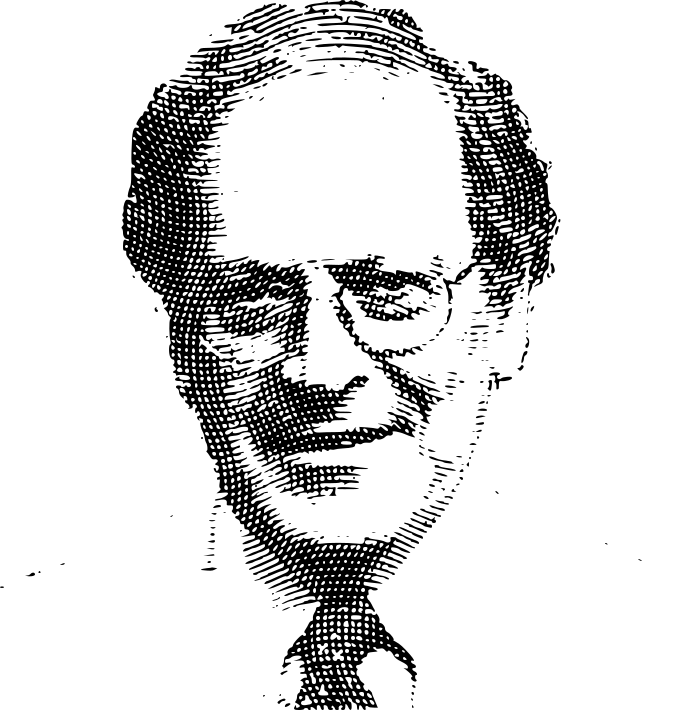
\includegraphics{Images/valiant.pdf}

}

\caption{\label{fig-valiant}Leslie Valiant received the Turing Award in
2010.}

\end{marginfigure}

Up to this point in the chapter, we have described MLT following {SLT}.
Now we will revisit some of what we already explained with the formalism
of the PAC model. The PAC model was proposed by Leslie Valiant
(Figure~\ref{fig-valiant}) in \(1984\)~(Valiant
1984)\marginpar{\begin{footnotesize}\leavevmode\vadjust pre{\protect\hypertarget{ref-valiant1984}{}}%
Valiant, L. G. 1984. {``A Theory of the Learnable.''} In
\emph{Proceedings of the Sixteenth Annual {ACM} Symposium on Theory of
Computing - 84}. {ACM} Press.
\url{https://doi.org/10.1145/800057.808710}.\vspace{2mm}\par\end{footnotesize}}.
The lack of citation to Vapnik and Chervonenkis literature is an
indication that the overlap of CoLT and STL was reinvented. As expected,
CoLT looks at the learning problem from a computational perspective,
while SLT from a statistical one.

``\emph{The PAC framework deals with the question of learnability for a
concept class \(\CC\) and not a particular concept''}~(Mohri,
Rostamizadeh, and Talwalkar
2012)\marginpar{\begin{footnotesize}\leavevmode\vadjust pre{\protect\hypertarget{ref-mohri2012}{}}%
Mohri, Mehryar, Afshin Rostamizadeh, and Ameet Talwalkar. 2012.
\emph{Foundations of Machine Learning}. The MIT Press.\vspace{2mm}\par\end{footnotesize}},
where a concept class is a set of concepts \(c_i\). The PAC model
classifies concept classes in terms of their complexities to achieve an
approximate solution; sample complexity, the number of examples needed,
computation complexity, the number of iterations needed.

In the PAC framework, a concept class \(\CC\) is learnable if there is
an algorithm capable of generating, with polynomial time and examples, a
general function (the hypothesis \(h\)) that with high confidence
(\(1-\delta\)), has an arbitrarily small error \(\epsilon\) in any given
instance of the problem.

\begin{longtable}[]{@{}
  >{\centering\arraybackslash}p{(\columnwidth - 4\tabcolsep) * \real{0.3662}}
  >{\centering\arraybackslash}p{(\columnwidth - 4\tabcolsep) * \real{0.3592}}
  >{\centering\arraybackslash}p{(\columnwidth - 4\tabcolsep) * \real{0.2606}}@{}}
\toprule()
\endhead
Probably & Aproximately & Correct \\
\(\scriptstyle \textrm{confidence} \geq(1-\delta)\) &
\({\scriptstyle \textrm{tolerance} \leq\epsilon}\) &
\(\scriptstyle {h(\cdot)=c(\cdot)}\) \\
\bottomrule()
\end{longtable}

If with absolute certainty, the hypothesis ``imitates'' the concept,
there is no error; we can say that there was learning:

\begin{align}
    \exists h \in \mathcal{H}: ~ \pr_{\mathit{x}\sim D}[c(\mathit{x})\neq h(\mathit{x})]=0 \to \text{learning}.
\end{align} Nevertheless, this definition is too restrictive. For
instance, if \(c \not \subset \mathcal{H}\), there is no way for any
\(h\) to perfectly imitate \(c\). So let us redefine learning with new
relaxed constraints to the absolute error:

\begin{align}
    &\pr_{x \sim D}{\Large\mathbb{1}}_{[c(\mathit{x}) \neq h(\mathit{x})]}= R_{D}(h)\\
    &\exists h \in \mathcal{H}:~ R_{D}(h) \leq \epsilon, ~ 0 < \epsilon < \tfrac{1}{2} \to \text{learning}.
\end{align}

Allowing some tolerance to error, however, is still not sufficient. On
one side, a \emph{hypothesis} does not need to be equal to the
\emph{concept} to be \textbf{\emph{consistent} to the sample}, to
correctly predict every example of the sample. In the figure
\textbf{?@fig-conceptVshypothesis}, the hypothesis was \emph{lucky}, and
there is no difference between the hypothesis and the concept for the
particular sample, even though they are different maps of
\(\mathcal{X}\).

On the other side, it is possible that the sample: \begin{align}
    S_n = \{(\mathit{x}_1,\mathit{y}_1), \cdots, (\mathit{x}_n, \mathit{y}_n)\} \sim D^n
\end{align} is \emph{unlucky}, and is a set of \emph{bad} examples for
the learning algorithm, an uninformative sample, making it impossible
for the hypothesis to \emph{imitate} the concept for all
\(\mathit{x}\in \mathcal{X}\). In this \emph{unlucky} case, learning
would be impossible. Hence, we relax the constraints once more:
\begin{align}
    \exists h \in \mathcal{H}, ~0 < \epsilon < \tfrac{1}{2}, ~0 < \delta < \tfrac{1}{2}: \nonumber\\
    ~\pr_{S \sim D^n}[R_{D}(h) > \epsilon] < \delta \to \text{learning}.
\end{align} Nevertheless, if achieving such thresholds demands an
unreasonable amount of data and time, can we say that learning has
happened? What is a reasonable amount of time and examples?

Let \(d\) be a number such that representing any vector
\(\mathit{x}\in \mathcal{X}\) costs at most \(\OO(d)\)
(\(\mathcal{X}= \mathbb{R}^d\)), and \(\operatorname{size}(c)\) the
computational cost of representing a concept \(c \in \CC\).

A concept class \(\CC\) is \textbf{PAC-learnable} if there is a learning
algorithm \(\mathcal{A}\) and a polynomial function
\(\operatorname{poly}(\cdot,\cdot, \cdot, \cdot, )\) such that for any
\(0< \epsilon < \tfrac{1}{2}\) and any \(0< \delta < \tfrac{1}{2}\), for
any distribution \(D\) on \(\mathcal{X}\) and for any target concept
\(c \in \CC\), the following holds for any sample size
\(n \geq \operatorname{poly}(\tfrac{1}{\epsilon}, \tfrac{1}{\delta}, d, \text{size}(c))\)~(Mohri,
Rostamizadeh, and Talwalkar
2012)\marginpar{\begin{footnotesize}\leavevmode\vadjust pre{\protect\hypertarget{ref-mohri2012}{}}%
Mohri, Mehryar, Afshin Rostamizadeh, and Ameet Talwalkar. 2012.
\emph{Foundations of Machine Learning}. The MIT Press.\vspace{2mm}\par\end{footnotesize}}:
\begin{align}
        \pr_{S \sim D^n}[R_{D}(h) \leq \epsilon] \geq (1 - \delta).
\end{align} If \(\mathcal{A}\) further runs in
\(\operatorname{poly}(\tfrac{1}{\epsilon}, \tfrac{1}{\delta}, d, \text{size}(c))\),
then \(\CC\) is said to be \textbf{efficiently PAC-learnable}. When such
an algorithm \(\mathcal{A}\) exists, it is called a \textbf{PAC-learning
algorithm} for \(\CC\)~(Mohri, Rostamizadeh, and Talwalkar
2012)\marginpar{\begin{footnotesize}\leavevmode\vadjust pre{\protect\hypertarget{ref-mohri2012}{}}%
Mohri, Mehryar, Afshin Rostamizadeh, and Ameet Talwalkar. 2012.
\emph{Foundations of Machine Learning}. The MIT Press.\vspace{2mm}\par\end{footnotesize}}.

\hypertarget{pac-bounds}{%
\section{PAC Bounds}\label{pac-bounds}}

As we stated before, one of the main goals of {MLT} is to guarantee
bounds to the error and the number of samples needed (sample complexity)
in learning problems. Here we present some of these guarantees as
examples of how this theoretical development allows us to make claims on
unknown distributions and unseen examples.

\hypertarget{guarantees-for-finite-hypothesis-spaces-consistent-case}{%
\subsection{Guarantees for finite hypothesis spaces --- consistent
case}\label{guarantees-for-finite-hypothesis-spaces-consistent-case}}

::: theorem \{\#thm-haussler\}

Let \(\mathcal{H}\) be a finite hypothesis space, \(\mathcal{A}\) a
learning algorithm that returns a consistent hypothesis \(h\),
i.e.~\(~\hat{R}_{S}(h)=0\), for any hypothesis \(h \in \mathcal{H}\) and
unknown distribution \(D=P(\mathit{X},\mathit{Y})\).\\

:::

Let \(|S|=n\), then, \(\forall n \geq 1\): \begin{align}
        \pr\,[\exists h \in \mathcal{H}: R_{D}(h)>\epsilon]\leq |\mathcal{H}| e^{-\epsilon n}
\end{align}

\begin{proof}

Let \(h_{\text{bad}} (\text{bad} = 1, ..., k)\) be all hypotheses in the
space \(\mathcal{H}_{\text{bad}} \subset \mathcal{H}\) where
\(\forall h_{\text{bad}} \in \mathcal{H}_{\text{bad}}: R_{D}(h_{\text{bad}})>\epsilon\),
then:

The chance of a \emph{bad} hypothesis to correctly predict an example
is: \begin{align}
        \pr_{\mathit{x}_j\sim S}\{{\Large\mathbb{1}}_{[(c(\mathit{x}_j) \neq h_{\text{bad}}(\mathit{x}_j))]}=\emptyset\} \leq (1-\epsilon) \\
        \pr_{\mathit{x}_j\sim S}[R_{\mathit{x}_j}(h_{\text{bad}})=0] \leq (1-\epsilon)
    \label{haussler:a} 
\end{align}

Therefore, the probability that a \emph{bad} hypothesis will predict all
examples correctly in the training sample \(S_n\) is: \begin{align}
        \pr_{\mathit{x}_1 \sim S}[R_{\mathit{x}_1}(h_{\text{bad}})=0] &\land\\
        \pr_{\mathit{x}_2 \sim S}[R_{\mathit{x}_2}(h_{\text{bad}})=0] &\land\\
        \nonumber \cdots\\
        \pr_{\mathit{x}_n \sim S}[R_{\mathit{x}_n}(h_{\text{bad}})=0] &\leq \underbrace{(1-\epsilon) \cdots (1-\epsilon)}_{n} \\
        \pr[(\hat{R}_{S}(h)=0) \land (R_{D}(h)> \epsilon)] &\leq (1-\epsilon)^n
    \label{haussler:b} 
\end{align} We said there are \(k\) \emph{bad} hypotheses, then, the
probability of any of these \emph{bad} hypothesis predicting all the
training sample correctly is: \begin{align}
        \pr\,[h_1 \in \mathcal{H}_{\text{bad}}: (\hat{R}_{S}(h_1)=0) \land (R_{D}(h)> \epsilon)] &\lor \\
        \pr\,[h_2 \in \mathcal{H}_{\text{bad}}: (\hat{R}_{S}(h_2)=0) \land (R_{D}(h)> \epsilon)] &\lor \\
        \ldots \nonumber \\
        \lor \pr\,[h_k \in \mathcal{H}_{\text{bad}}: (\hat{R}_{S}(h_k)=0) \land (R_{D}(h)> \epsilon)] &
        \leq \sum_{1}^k (1-\epsilon)^n\\
        \pr\,[\exists h \in H: (\hat{R}_{S}(h)=0) \land (R_{D}(h)>\epsilon)] &\leq k (1-\epsilon)^n
    \label{haussler:c} 
\end{align} Finally, as these \emph{bad} hypotheses belong to
\(\mathcal{H}_{\text{bad}} \subset \mathcal{H}\), \(k < |\mathcal{H}|\),
therefore, we get the theoretical error of \(h\) given a precision
tolerance of \(\epsilon\), and sample complexity of \(n\) examples:
\begin{align}
        \pr\,[\exists h \in \mathcal{H}: R_{D}(h)>\epsilon]&\leq |\mathcal{H}| (1-\epsilon)^n\label{haussler:d}\\
        (1-x) \leq e^{-x},&~0 \leq x \leq 1 \implies \nonumber\\
        \pr\,[\exists h \in \mathcal{H}: R_{D}(h)>\epsilon]&\leq |\mathcal{H}|e^{-\epsilon n} \nonumber
    
\end{align} ~◻

\end{proof}

From the PAC framework: \begin{align}
    \pr\,[\exists h \in \mathcal{H}: R_{D}(h)>\epsilon] < \delta
\end{align} Therefore, Haussler theorem gives us a lower bound on the
confidence: \begin{align}
    \delta > |\mathcal{H}|e^{-\epsilon n} \geq \pr\,[\exists h \in \mathcal{H}: R_{D}(h)>\epsilon]\label{eq:delta}
\end{align}

We can rewrite Haussler's theorem to bound the number of examples needed
for learning:

\protect\hypertarget{th-sample_complexity}{}{}A learning algorithm
\(\mathcal{A}\) can learn a concept \(c\) from a class of concepts
\(\CC\) with
\(n < \frac{1}{\epsilon}(\ln{|\mathcal{H}|}+\ln{\frac{1}{\delta}})\)
training examples.

\begin{proof}

\begin{align}
    \delta &> |H|e^{-\epsilon n} \\
    e^{-\epsilon n} &< \frac{\delta}{|\mathcal{H}|}\\
    - \epsilon n &< (\ln{\delta} - \ln{|\mathcal{H}|}) \\
    \epsilon n &< (\ln{|\mathcal{H}|} - \ln{\delta}) \\
    n &< \frac{1}{\epsilon}\left(\ln{|\mathcal{H}|} + \ln{\frac{1}{\delta}}\right) \\
    n \in &\OO \left( \frac{1}{\epsilon}(\ln{|\mathcal{H}|} + \ln{\frac{1}{\delta}}) \right)\tag{Sample complexity}
\end{align} ◻

\end{proof}

Strangely, the sample complexity upper bound does not depend on \(\CC\)
or \(D\) but depends logarithmically on the size of
\(\mathcal{H}\)~(Haussler
1988)\marginpar{\begin{footnotesize}\leavevmode\vadjust pre{\protect\hypertarget{ref-haussler1988}{}}%
Haussler, David. 1988. {``Quantifying Inductive Bias: AI Learning
Algorithms and Valiant's Learning Framework.''} \emph{Artificial
Intelligence} 36 (2): 177--221.\vspace{2mm}\par\end{footnotesize}}.

\hypertarget{no-free-lunch-theorem}{%
\subsection{No free lunch theorem}\label{no-free-lunch-theorem}}

\hypertarget{is-a-universal-concept-class-learnable}{%
\paragraph{Is a universal concept class
learnable?}\label{is-a-universal-concept-class-learnable}}

Let \(\mathcal{X}=\{0,1\}^{d}\), the space of Boolean vectors of size
\(d\). A universal concept class \(\UU_d\) has all subsets of
\(\mathcal{X}\), i.e.~contains all possible classifications for a given
instance space \(\mathcal{X}\). \begin{align}
    |\UU_d| = 2^{|\mathcal{X}|}&=2^{(2^d)} \\
    |\mathcal{H}| &\geq |\UU_d| \\
    |\mathcal{H}| &\geq 2^{(2^d)}
\end{align} From : \begin{align}
    n &\in \OO \biggl( \frac{1}{\epsilon}(\ln{|\mathcal{H}|} + \ln{\frac{1}{\delta}})\biggr)\\
    n &\in \OO \biggl( \frac{1}{\epsilon}\left(2^d \ln(2) + \ln{\frac{1}{\delta}}\right)\biggr) \therefore\\
    n &\in \OO \biggl( 2^d; \frac{1}{\epsilon}; \ln{\frac{1}{\delta}} \biggr)
\end{align} Therefore, the sample complexity is not polynomial to \(d\),
and \textbf{\(\UU_d\) is not PAC Learnable}. Moreover, the ``no free
lunch'' theorem~(Wolpert and Macready
1997)\marginpar{\begin{footnotesize}\leavevmode\vadjust pre{\protect\hypertarget{ref-wolpert1997}{}}%
Wolpert, David H., and William G. Macready. 1997. {``No Free Lunch
Theorems for Optimization.''} \emph{IEEE Transactions on Evolutionary
Computation} 1 (1): 67--82.\vspace{2mm}\par\end{footnotesize}}
states there is no universal concept, therefore, no universal learning
algorithm for all tasks. Specifically, averaged over all possible data
generating distributions, every classification algorithm achieves the
same error when classifying previously unknown points.

\hypertarget{guarantees-for-finite-hypothesis-spaces-inconsistent-case}{%
\subsection{Guarantees for finite hypothesis spaces --- inconsistent
case}\label{guarantees-for-finite-hypothesis-spaces-inconsistent-case}}

Usually, there is no hypothesis in \(\mathcal{H}\) consistent with the
training sample due to the stochastic nature of the supervisor or due to
the concept class being more complex than the hypothesis class used by
the learning algorithm.

To derive bounds for this inconsistent case, we will use the ``law of
large numbers''.

\hypertarget{law_of_large_numbers}{%
\paragraph{Law of large numbers}\label{law_of_large_numbers}}

The law of large numbers states that the mean of random variables
\(\xi_i\), drawn i.i.d. from some probability distribution \(P\),
converges to the mean of \(P\) itself when the sample size goes to
infinity. \begin{align}
    &\text{for}~n \to \infty, \nonumber\\
    &\frac{1}{n} \sum_{i=1}^{n}\xi_i \to \mathbb{E}(\xi), \xi_i \sim P.
\end{align}

Based on the fact that a statistic\sidenote{\footnotesize Remember: A statistic is a
  function of random variables that does not depend on parameters.} of
random variables can be treated itself as a random variable, we can make
the loss function \(\ell(\mathit{x}, \mathit{y}, h(\mathit{x}))\) be the
random variable \(\xi\) from above. From what we can conclude that for a
fixed \(h\), the empirical risk converges to the theoretical risk as the
sample size goes to infinity: \begin{align}
    &\text{for}~n \to \infty, \nonumber\\
    &\hat{R}_{S}(h) = \frac{1}{n} \sum_{i=1}^{n}(\ell(\mathit{x}_i, \mathit{y}_i, h(\mathit{x}_i)) \to \mathbb{E}(\ell(x, y, h(\mathit{x}))=R(h).
\end{align}

\hypertarget{sec-chernoff}{%
\paragraph{Chernoff-Hoeffding inequality}\label{sec-chernoff}}

Moreover, we can use the famous \emph{Chernoff-Hoeffding's inequality}
to bound the approximation of the risk:

\begin{align}
\pr\,\left(\Bigg | \frac{1}{n} \sum_{i=1}^{n}\xi_i - \mathbb{E}(\xi) \Bigg | \geq \epsilon \right) &\leq 2 e^{(-2n\epsilon^2)} \\
 \pr\,(|\hat{R}_{S}(h) - R(h)| \geq \epsilon) &\leq 2 e^{(-2n\epsilon^2)}
\end{align}

Unfortunately, this bound only holds for a fixed-function \(h\) which
does not depend on the training data, but our hypothesis certainly does
depend. The reason for such constraint is intuitive. If we let the
hypothesis space convey all possible functions and do not restrict our
hypothesis to be independent of the training data, we can always
generate a function that ``memorises'' the given sample and has no
empirical error. Such function will most certainly not generalise well
and invalidate the bound.

Vapnik and Chervonenkis solved this conundrum by using the Union bound.

\hypertarget{union-bound}{%
\paragraph{Union bound}\label{union-bound}}

Even if we are not allowed to select a hypothesis from the space using
training data, the bound still holds for any hypothesis took at random.
Also, if we enumerate all the functions in \(\mathcal{H}\), using the
fact that it is finite, the bound still holds for each hypothesis:
\begin{align}
    \pr\,(|\hat{R}_{S}(h_1) - R(h_1) | > &\epsilon~  \lor \nonumber \\
    |\hat{R}_{S}(h_2)-R(h_2)| > &\epsilon  \lor \cdots \nonumber \\
    \cdots \lor  |\hat{R}_{S}(h_{|\mathcal{H}|})-R(h_{|\mathcal{H}|}) > &\epsilon) \leq \sum^{|\mathcal{H}|} 2 e^{(-2n\epsilon^2)}\\    \therefore \pr\,\left[ \exists h \in \mathcal{H}:~|\hat{R}_{S}(h) - R(h)| >\epsilon\right] &\leq \sum^{|\mathcal{H}|} 2 e^{(-2n\epsilon^2)} \\
    \pr\,\left[ \exists h \in \mathcal{H}:~|\hat{R}_{S}(h) - R(h)| >\epsilon\right] &\leq 2 |\mathcal{H}| e^{(-2n\epsilon^2)}
\label{eq:union_bound} 
\end{align}

\protect\hypertarget{thrm:finite-inconsistent}{}{} Let \(\mathcal{H}\)
be a finite hypothesis class. Then, for any
\(0 < \delta < \tfrac{1}{2}\), with a probability at least \(1-\delta\),
the following inequality holds~(Mohri, Rostamizadeh, and Talwalkar
2012)\marginpar{\begin{footnotesize}\leavevmode\vadjust pre{\protect\hypertarget{ref-mohri2012}{}}%
Mohri, Mehryar, Afshin Rostamizadeh, and Ameet Talwalkar. 2012.
\emph{Foundations of Machine Learning}. The MIT Press.\vspace{2mm}\par\end{footnotesize}}:

\begin{align}
        \forall h \in \mathcal{H},~&R(h)\leq \hat{R}_{S}(h) + \epsilon \nonumber \\
        &R(h)\leq \hat{R}_{S}(h) + \sqrt{\frac{\ln{|\mathcal{H}|}+ \ln{2/\delta}}{2n}}
    
\end{align}

\begin{proof}

\begin{align}
        \pr\,\left[ \exists h \in \mathcal{H}:~|\hat{R}_{S}(h) - R(h)| >\epsilon\right] &< \delta \tag{from PAC}\\
        \pr\,\left[ \exists h \in \mathcal{H}:~|\hat{R}_{S}(h) - R(h)| >\epsilon\right] &\leq 2 |\mathcal{H}| e^{(-2n\epsilon^2)} \tag{from \eqref{eq:union_bound}\\
        \therefore \delta &> 2 |\mathcal{H}| e^{(-2n\epsilon^2)}
\end{align}

Assuming \(\delta = 2 |\mathcal{H}| e^{(-2n\epsilon^2)}\), we have:
\begin{align}
        e^{(-2n\epsilon^2)} = \frac{\delta}{2|\mathcal{H}|} \\
        -2n\epsilon^2 = \ln{\delta} - ln{2|\mathcal{H}|}\\
        \epsilon^2 = \frac{\ln{|\mathcal{H}|}+\ln{2}-\ln{\delta}}{2n}\\
        \therefore \epsilon > 0 \rightarrow \epsilon = + \sqrt{\frac{\ln{|\mathcal{H}|}+ \ln{2/\delta}}{2n}}\label{eq:epsilon_ch}
    
\end{align} By definition, \(R(h)\geq \hat{R}_{S}(h)\), thus:
\begin{align}
        \pr\,\left[ \exists h \in \mathcal{H}:~(R(h) - \hat{R}_{S}(h)) >\epsilon\right] &< \delta \\
        \pr\,\left[ \forall h \in \mathcal{H}:~(R(h) - \hat{R}_{S}(h)) \leq \epsilon\right] &\geq 1 - \delta
    
\end{align} Therefore, with probability at least \(1-\delta\):
\begin{align}
        \forall h \in \mathcal{H}, R(h)&\leq \hat{R}_{S}(h) + \epsilon \\
        \forall h \in \mathcal{H}, R(h)&\leq \hat{R}_{S}(h) + \sqrt{\frac{\ln{|\mathcal{H}|}+ \ln{2/\delta}}{2n}} \\
        \forall h \in \mathcal{H}, R(h)&\leq \hat{R}_{S}(h) + \OO \left(\sqrt{ \log |\mathcal{H}| }; \sqrt{1/n}; \sqrt{ \log 1/\delta} \right) \nonumber
    
\end{align}~◻

\end{proof}

We can rewrite to bound the sample complexity:

A learning algorithm \(\mathcal{A}\) can learn a concept \(c\) from a
class of concepts \(\CC\) with
\(n \leq \frac{\ln{|\mathcal{H}|}+\ln{\frac{2}{\delta}}}{2\epsilon^2}\)
training examples.

\begin{proof}

\begin{align}
        \epsilon \leq \sqrt{\frac{\ln{|\mathcal{H}|}+ \ln{2/\delta}}{2n}}
        \therefore n \leq \frac{\ln{|\mathcal{H}|}+ \ln{2/\delta}}{2\epsilon^2} \nonumber
    
\end{align}~◻

\end{proof}

\hypertarget{guarantees-for-infinite-hypothesis-space-inconsistent-case}{%
\subsection{Guarantees for infinite hypothesis space --- inconsistent
case}\label{guarantees-for-infinite-hypothesis-space-inconsistent-case}}

It can be argued that for our use in machine learning, there is no need
for guarantees for infinite \(\mathcal{H}\) due to the nature of
computer hardware and their memory limitations, which already discretise
the hypothesis spaces. Anyway, we will give a general idea of this case.

One of the most striking insights of Vapnik and Chervonenkis is the idea
of the \emph{shattering coefficient} (\(\NN\)). Let us take a look at
the bound from : \begin{align}
    \forall h \in \mathcal{H}, ~~
    R(h)\leq \hat{R}_{S}(h) + \sqrt{\frac{\ln{|\mathcal{H}|}+ \ln{2/\delta}}{2n}} \nonumber \\
\end{align} The \(\ln |\mathcal{H}|\) relates to \(d\), the size of the
\emph{representation} of the hypothesis space. Another remark worth
mentioning is that in the union bound, we just added the probabilities
of each \(h_i \in \mathcal{H}\) without considering where
\(P(h_j) \cap P(h_k), j \neq k\).

begin\{figure\} {[}ht!{]} \centering

\begin{venndiagram2sets}
        [tikzoptions={thick},shade={}, radius=0.8cm, labelA={}, labelB={}]
        \begin{scope}[every path/.append style={pattern=north east lines}]
        \fillA
        \end{scope}
        \begin{scope}[every path/.append style={pattern=north west lines}]
            \fillB
        \end{scope}
        \draw (0.5,2) node {{\(h_j~~~\)}};
        \draw (3,2) node {{\(~~h_k\)}};
    \end{venndiagram2sets}
    \caption{\(\pr(h_j) \cap \pr(h_k)\) is summed twice in the union bound.}
\label{fig:join_probability}

\textbackslash end\{figure\}

In reality, there are several different \(h \in \mathcal{H}\) that
provide the same map \(x \in S \to y \in \{-, +\}\). Therefore, the
effective size of \(\mathcal{H}\) is smaller than \(|\mathcal{H}|\).
Using a symmetrisation trick~(Von Luxburg and Schölkopf 2011, sec.
5.2)\marginpar{\begin{footnotesize}\leavevmode\vadjust pre{\protect\hypertarget{ref-luxburg2011}{}}%
Von Luxburg, Ulrike, and Bernhard Schölkopf. 2011. {``Statistical
Learning Theory: Models, Concepts, and Results.''} In \emph{Handbook of
the History of Logic}, 10:651--706. Elsevier.\vspace{2mm}\par\end{footnotesize}},
Vapnik and Chervonenkis showed that there are at most \(2^{2n}\)
effectively different hypotheses. In the PAC framework,
\(|\mathcal{Y}|=2\), so if a pattern is a set \(\{y_1,\cdots,y_n\}\),
there are \(|\mathcal{H}|=2^n\) different patterns, thus, effectively
different hypotheses.This number, however, can be even smaller; for
example, a certain \(y_k, k<n\) can, for example, only accept a specific
value, \(y_k={+}\).

The shattering coefficient is a growth function, it measures the number
of effectively distinct hypotheses as the sample size \(n\) grows. It is
a capacity measure of a hypothesis class. Whenever
\(\NN(\mathcal{H}, n)=2^n\), there exists a sample of size \(n\) on
which all possible separations of the patterns can be achieved by some
\(h \in \mathcal{H}\).

We can now rewrite as: \begin{align}
    \forall h \in \mathcal{H}&,\nonumber\\
    R(h)&\leq \hat{R}_{S}(h) + \sqrt{\frac{\ln{\NN(\mathcal{H}, n)}+ \ln{2/\delta}}{2n}}
\end{align} Another capacity measure is the famous VC
dimension.\sidenote{\footnotesize Named after Vapnik and Chervonenkis.} \begin{align}
    \operatorname{VC}(\mathcal{H})=max\{n \in \mathbb{N}| \NN(\mathcal{H}, n)=2^n \text{ for some }S_n\}
\end{align} A combinatorial result relates the growth behaviour of the
shattering coefficient with the VC dimension:

\begin{align}
        \text{If }&\operatorname{VC}(\mathcal{A})=d, \forall n \geq 1,\nonumber
         ~&\NN(\mathcal{H}, n) \leq \sum_{k=0}^d \binom{n}{k} \leq\left(\frac{\epsilon n}{d}\right)^d
    
\end{align}

\hypertarget{minimum-description-length}{%
\section{Minimum Description Length}\label{minimum-description-length}}

{MDL} is an {MLT} principle proposed by Hinton and Van Camp
(1993)\marginpar{\begin{footnotesize}\leavevmode\vadjust pre{\protect\hypertarget{ref-hinton1993}{}}%
Hinton, Geoffrey E, and Drew Van Camp. 1993. {``Keeping the Neural
Networks Simple by Minimizing the Description Length of the Weights.''}
In \emph{Proceedings of the Sixth Annual Conference on Computational
Learning Theory}, 5--13.\vspace{2mm}\par\end{footnotesize}}~(Hinton
and Van Camp
1993)\marginpar{\begin{footnotesize}\leavevmode\vadjust pre{\protect\hypertarget{ref-hinton1993}{}}%
Hinton, Geoffrey E, and Drew Van Camp. 1993. {``Keeping the Neural
Networks Simple by Minimizing the Description Length of the Weights.''}
In \emph{Proceedings of the Sixth Annual Conference on Computational
Learning Theory}, 5--13.\vspace{2mm}\par\end{footnotesize}}.
It will be presented later ({[}{[}sec:mdl{]}{]}{[}9{]}) as it relates to
Information Theory.

\hypertarget{sec-pac-bayes}{%
\section{PAC-Bayes}\label{sec-pac-bayes}}

For a long time, {MLT} was divided between Bayesian inference and PAC
learning. In 1997, Shawe-Taylor and Williamson
(1997)\marginpar{\begin{footnotesize}\leavevmode\vadjust pre{\protect\hypertarget{ref-shawe-taylor1997}{}}%
Shawe-Taylor, John, and Robert C Williamson. 1997. {``A PAC Analysis of
a Bayesian Estimator.''} In \emph{Proceedings of the Tenth Annual
Conference on Computational Learning Theory}, 2--9.\vspace{2mm}\par\end{footnotesize}}
first presented a theorem of PAC guarantees for Bayesian algorithms
(algorithms that minimise the risk using a prior probability for the
data and hypothesis)(Shawe-Taylor and Williamson
1997)\marginpar{\begin{footnotesize}\leavevmode\vadjust pre{\protect\hypertarget{ref-shawe-taylor1997}{}}%
Shawe-Taylor, John, and Robert C Williamson. 1997. {``A PAC Analysis of
a Bayesian Estimator.''} In \emph{Proceedings of the Tenth Annual
Conference on Computational Learning Theory}, 2--9.\vspace{2mm}\par\end{footnotesize}}.
This bridge allowed tighter PAC bounds for learning algorithms that take
advantage of informative priors. Here we give PAC Bayes bounds for
finite hypothesis spaces (for more, see (McAllester
1999)\marginpar{\begin{footnotesize}\leavevmode\vadjust pre{\protect\hypertarget{ref-mcallester1999}{}}%
McAllester, David A. 1999. {``Some PAC-Bayesian Theorems.''}
\emph{Machine Learning} 37 (3): 355--63.
\url{https://doi.org/10.1023/a1007618624809}.\vspace{2mm}\par\end{footnotesize}}
and (McAllester
2013)\marginpar{\begin{footnotesize}\leavevmode\vadjust pre{\protect\hypertarget{ref-mcallester2013}{}}%
---------. 2013. {``A PAC-Bayesian Tutorial with {A} Dropout Bound.''}
\emph{CoRR} abs/1307.2118. \url{https://arxiv.org/abs/1307.2118}.\vspace{2mm}\par\end{footnotesize}}).

\hypertarget{pac-bayes-guarantees-for-finite-hypothesis-spaces-consistent-case}{%
\subsection{PAC Bayes Guarantees for finite hypothesis spaces ---
consistent
case}\label{pac-bayes-guarantees-for-finite-hypothesis-spaces-consistent-case}}

Let \(\mathcal{H}\) be a finite hypothesis space, \(\mathcal{A}\) a
learning algorithm that returns a consistent hypothesis \(h\),
i.e.\(\hat{R}_{S}(h)=0\), for any hypothesis \(h\) and unknown
distribution \(D=P(\mathit{X},\mathit{Y})\), any \(|S|=n: n \geq 1\).
For any probability distribution \(P\) assigning a nonzero probability
to every hypothesis in the finite hypothesis space \(\mathcal{H}\), with
confidence \(1-\delta\) over the selection of the sample of \(n\)
instances the following holds true:\\

\begin{align}
        \pr\,[h \in H: (\hat{R}_{S}(h)=0) \land (R_{D}(h)>\epsilon)]\leq \frac{\ln \frac{1}{P(h)}+ \ln \frac{1}{\delta}}{n}
    
\end{align}

\begin{proof}

This proof is very similar to the one in \textbf{?@thm-haussler}. From
{[}{[}haussler:c{]}{]}{[}10{]}: \begin{align}
        \pr\,[h \in H: (\hat{R}_{S}(h)=0) \land (R_{D}(h)>\epsilon)] &\leq (1-\epsilon)^n,
    
\end{align} But we also know that: \begin{align}
        \pr\,[h \in H: (\hat{R}_{S}(h)=0) \land (R_{D}(h)>\epsilon)] &\leq P(h)\delta\\
        (1-x) \leq e^{-x},~0 \leq x \leq 1 \implies 
        e^{-\epsilon n} &< P(h) \delta\\
        \epsilon &< \frac{\ln \frac{1}{P(h)}+ \ln \frac{1}{\delta}}{n}  \nonumber
    
\end{align} ◻

\end{proof}

\hypertarget{pac-bayes-guarantees-for-finite-hypothesis-spaces-inconsistent-case}{%
\subsection{PAC Bayes Guarantees for finite hypothesis spaces ---
inconsistent
case}\label{pac-bayes-guarantees-for-finite-hypothesis-spaces-inconsistent-case}}

\protect\hypertarget{thrm:pac-bayes}{}{}Let \(\mathcal{H}\) be a finite
hypothesis space, \(\mathcal{A}\) a learning algorithm that returns a
hypothesis \(h\) given a sample \(|S|=n: n \geq 1\) from the unknown
distribution \(D=P(\mathit{X},\mathit{Y})\). Given a probability
distribution \(P\) assigning nonzero probability
\(\forall h \in \mathcal{H}\), with confidence \((1-\delta)\) the
following holds:\\
\begin{align}
        \forall h \in \mathcal{H},~R(h)\leq\hat{R}_{S}(h) + \sqrt{\frac{\ln{\frac{1}{P(h)}}+ \ln{\frac{2}{\delta}}}{2n}}
    
\end{align}

\begin{proof}

As in , we need to apply the union bound over the Chernoff bound:
\begin{align}
        \pr\,[h \in H: (\hat{R}_{S}(h_1)=0) \land (R_{D}(h)>\epsilon)] &\leq 2e^{(-2n\epsilon^2)},
    
\end{align} But we also know that: \begin{align}
        \pr\,[h \in H: (\hat{R}_{S}(h)=0) \land (R_{D}(h)>\epsilon)] &\leq P(h)\delta \\
        2e^{(-2n\epsilon^2)} &< P(h) \delta\\
        \epsilon &< \sqrt{\frac{\ln{\frac{1}{P(h)}}+ \ln{\frac{2}{\delta}}}{2n}} \nonumber
    
\end{align} ◻

\end{proof}

\hypertarget{sec-mlt_criticism}{%
\section{Critiques on MLT}\label{sec-mlt_criticism}}

This dissertation aims to present an emergent new theory for
understanding Deep Learning. In this context, we should first ask
ourselves: \textbf{Is anything wrong with the current {MLT}? Do we
really need a new theory?}

Truth be told: we did not cover \emph{current} {MLT} in this chapter
which aimed to be an introductory overview of the subject. There are
many topics in active development beyond what was presented here:
Structural Risk Minimisation, Rademacher complexity, Uniform Stability,
for example.

With this caveat, here we digest some of the critiques on the current
state of MLT in two parts, one for general critiques and another for
critiques specific to the case of Deep Learning.

\hypertarget{sec-general_critiques}{%
\subsection{General critiques}\label{sec-general_critiques}}

\hypertarget{no-assumption-on-dpmathitxmathity-see-assumptions11-assumption-distribution-free12}{%
\paragraph{\texorpdfstring{No assumption on
\(D=P(\mathit{X},\mathit{Y})\) (see {[}{[}assumptions{]}{]}{[}11{]},
assumption
{[}{[}distribution-free{]}{]}{[}12{]}):}{No assumption on D=P(\textbackslash mathit\{X\},\textbackslash mathit\{Y\}) (see {[}{[}assumptions{]}{]}{[}11{]}, assumption {[}{[}distribution-free{]}{]}{[}12{]}):}}\label{no-assumption-on-dpmathitxmathity-see-assumptions11-assumption-distribution-free12}}

One of the assumptions of classical learning theory is that ``there are
no assumptions on \(D=P(\mathit{X},\mathit{Y})\)''. Although this
assumption means that MLT bounds guarantee approximation to any
arbitrary distribution; distributions of practical interest are the ones
found in Nature. These practical distributions have some peculiar
characteristics that physicists know about(Lin, Tegmark, and Rolnick
2017)\marginpar{\begin{footnotesize}\leavevmode\vadjust pre{\protect\hypertarget{ref-lin2016}{}}%
Lin, Henry W, Max Tegmark, and David Rolnick. 2017. {``Why Does Deep and
Cheap Learning Work so Well?''} \emph{Journal of Statistical Physics}
168 (6): 1223--47.\vspace{2mm}\par\end{footnotesize}}:
Low polynomial order, locality, symmetry, among others.

\hypertarget{absence-of-the-notion-of-timesee-assumptions11-assumption-no-time13}{%
\paragraph{Absence of the notion of ``time''(see
{[}{[}assumptions{]}{]}{[}11{]}, assumption
{[}{[}no-time{]}{]}{[}13{]}):}\label{absence-of-the-notion-of-timesee-assumptions11-assumption-no-time13}}

One of MLT assumptions on \(P(\mathit{X},\mathit{Y})\) is that it is
fixed; there is no ``time'' parameter. Several practical uses of machine
learning are in data streams where it is common to have one observation
affecting the probability of the future ones~(Mello and Ponti
2018)\marginpar{\begin{footnotesize}\leavevmode\vadjust pre{\protect\hypertarget{ref-mello2018}{}}%
Mello, Rodrigo F., and Moacir Antonelli Ponti. 2018. \emph{Machine
Learning: A Practical Approach on the Statistical Learning Theory}.
Springer.\vspace{2mm}\par\end{footnotesize}}.

\hypertarget{identically-independent-sampling-see-assumptions11-assumption-independent_sampling14}{%
\paragraph{Identically Independent sampling (see
{[}{[}assumptions{]}{]}{[}11{]}, assumption
{[}{[}independent\_sampling{]}{]}{[}14{]}):}\label{identically-independent-sampling-see-assumptions11-assumption-independent_sampling14}}

One of the assumptions of Machine Learning is that the datasets are
sampled i.i.d. This sampling assumption is often violated in practice;
for example, a machine learning medical application may use data from
one hospital to train a model that will be applied worldwide.

The violations are, of course, of practical reasons. However, up to what
point can we say that a particular dataset is i.i.d.? Let us think over
the problem of facial recognition. Taking photos at random in a
university is not i.i.d because the people that goes to the university
is a limited set of the whole population. If we use random images on the
Internet, we may only get the kind of picture people chose to display, a
bias of intention. There is always some bias in any dataset: a
selection, intention bias or technical bias (due to the image capture
device).

\hypertarget{arbitrary-loss-metrics}{%
\paragraph{Arbitrary Loss metrics}\label{arbitrary-loss-metrics}}

In {MLT} learning setting, the choice of the loss function is arbitrary,
which curbs any objective, metric-independent interpretation of the
results.

\hypertarget{blackbox}{%
\paragraph{Black-box analysis}\label{blackbox}}

In {MLT}, the model is treated as a black-box ~(Alain and Bengio
2016)\marginpar{\begin{footnotesize}\leavevmode\vadjust pre{\protect\hypertarget{ref-alain2016}{}}%
Alain, Guillaume, and Yoshua Bengio. 2016. {``Understanding Intermediate
Layers Using Linear Classifier Probes.''} \emph{arXiv Preprint
arXiv1610.01644}.\vspace{2mm}\par\end{footnotesize}}
(as cited by ~(Shwartz-Ziv and Tishby
2017)\marginpar{\begin{footnotesize}\leavevmode\vadjust pre{\protect\hypertarget{ref-shwartz-ziv2017}{}}%
Shwartz-Ziv, Ravid, and Naftali Tishby. 2017. {``Opening the Black Box
of Deep Neural Networks via Information.''}
\url{https://arxiv.org/abs/1703.00810}.\vspace{2mm}\par\end{footnotesize}}),
the analysis is based only on the input and the output of the model.

\hypertarget{in-specific-for-deep-learning}{%
\subsection{In specific for Deep
Learning}\label{in-specific-for-deep-learning}}

\hypertarget{vacuous-bounds}{%
\paragraph{Vacuous bounds}\label{vacuous-bounds}}

Machine Learning Theory cannot explain deep neural networks
generalisation performance. According to MLT, the deep learning
generalisation gap is in \(\OO(|\theta| \log |\theta|)\), where
\(|\theta|\) is the number of parameters of the network~(Kakade and
Tewari
2008)\marginpar{\begin{footnotesize}\leavevmode\vadjust pre{\protect\hypertarget{ref-kakade2008}{}}%
Kakade, Sham, and Ambuj Tewari. 2008. {``VC Dimension of Multilayer
Neural Networks, Range Queries.''} The University of Chicago.
\url{https://ttic.uchicago.edu/~tewari/lectures/lecture12.pdf}.\vspace{2mm}\par\end{footnotesize}}.
These bounds are vacuous by orders of magnitudes~(Zhou et al. 2019;
Zhang et al.
2016)\marginpar{\begin{footnotesize}\leavevmode\vadjust pre{\protect\hypertarget{ref-zhou2019}{}}%
Zhou, Wenda, Victor Veitch, Morgane Austern, Ryan P. Adams, and Peter
Orbanz. 2019. {``Non-Vacuous Generalization Bounds at the ImageNet
Scale: A {PAC}-Bayesian Compression Approach.''} In \emph{International
Conference on Learning Representations}.\vspace{2mm}\par\end{footnotesize}}\marginpar{\begin{footnotesize}\leavevmode\vadjust pre{\protect\hypertarget{ref-zhang2016}{}}%
Zhang, Chiyuan, Samy Bengio, Moritz Hardt, Benjamin Recht, and Oriol
Vinyals. 2016. {``Understanding Deep Learning Requires Rethinking
Generalization.''} \url{https://arxiv.org/abs/1611.03530}.\vspace{2mm}\par\end{footnotesize}}.
However, deeper and larger networks consistently show better
generalisation performance than smaller ones.

\hypertarget{inexplicable-phenomena}{%
\paragraph{``Inexplicable'' phenomena}\label{inexplicable-phenomena}}

{DL} has several phenomena with no definitive explanation, stemming from
a single narrative. For example:

\begin{itemize}
\item
  Generalisation with the addition of layers: as we explained in this
  chapter, the current {MLT} expects models with fewer parameters to
  generalise better; that is not what happens in {DL}. Moreover,~Zhang
  et al.
  (2016)\marginpar{\begin{footnotesize}\leavevmode\vadjust pre{\protect\hypertarget{ref-zhang2016}{}}%
Zhang, Chiyuan, Samy Bengio, Moritz Hardt, Benjamin Recht, and Oriol
Vinyals. 2016. {``Understanding Deep Learning Requires Rethinking
Generalization.''} \url{https://arxiv.org/abs/1611.03530}.\vspace{2mm}\par\end{footnotesize}}
  showed that the hypothesis space of {DNN} is large enough to allow
  convergence to random labels~(Zhang et al.
  2016)\marginpar{\begin{footnotesize}\leavevmode\vadjust pre{\protect\hypertarget{ref-zhang2016}{}}%
Zhang, Chiyuan, Samy Bengio, Moritz Hardt, Benjamin Recht, and Oriol
Vinyals. 2016. {``Understanding Deep Learning Requires Rethinking
Generalization.''} \url{https://arxiv.org/abs/1611.03530}.\vspace{2mm}\par\end{footnotesize}}.
\item
  Disentanglement of semantic factors: the representation of the input
  in deep layers usually disentangle semantic factors, different
  semantic factors are not strongly correlated in the representation;
\item
  Superconvergence:~Smith and Topin
  (2019)\marginpar{\begin{footnotesize}\leavevmode\vadjust pre{\protect\hypertarget{ref-smith2019}{}}%
Smith, Leslie N., and Nicholay Topin. 2019. {``Super-Convergence: Very
Fast Training of Neural Networks Using Large Learning Rates.''} In
\emph{Artificial Intelligence and Machine Learning for Multi-Domain
Operations Applications}, 11006:1100612. International Society for
Optics; Photonics.\vspace{2mm}\par\end{footnotesize}}
  present that overall training time can be shortened and better
  accuracy achieved by cyclical learning rates~(Smith and Topin
  2019)\marginpar{\begin{footnotesize}\leavevmode\vadjust pre{\protect\hypertarget{ref-smith2019}{}}%
Smith, Leslie N., and Nicholay Topin. 2019. {``Super-Convergence: Very
Fast Training of Neural Networks Using Large Learning Rates.''} In
\emph{Artificial Intelligence and Machine Learning for Multi-Domain
Operations Applications}, 11006:1100612. International Society for
Optics; Photonics.\vspace{2mm}\par\end{footnotesize}}.~Howard
  and Ruder
  (2018)\marginpar{\begin{footnotesize}\leavevmode\vadjust pre{\protect\hypertarget{ref-howard2018universal}{}}%
Howard, Jeremy, and Sebastian Ruder. 2018. {``Universal Language Model
Fine-Tuning for Text Classification.''} In \emph{ACL}. Association for
Computational Linguistics. \url{http://arxiv.org/abs/1801.06146}.\vspace{2mm}\par\end{footnotesize}}
  propose a slight variation of the method, slanted triangular learning
  rates, and achieve even better performance~(Howard and Ruder
  2018)\marginpar{\begin{footnotesize}\leavevmode\vadjust pre{\protect\hypertarget{ref-howard2018universal}{}}%
Howard, Jeremy, and Sebastian Ruder. 2018. {``Universal Language Model
Fine-Tuning for Text Classification.''} In \emph{ACL}. Association for
Computational Linguistics. \url{http://arxiv.org/abs/1801.06146}.\vspace{2mm}\par\end{footnotesize}}.
  This superconvergence phenomenon is not well studied, and there are
  only a few conjectures on why it does happen.
\item
  Critical Learning Periods:~Achille, Rovere, and Soatto
  (2017)\marginpar{\begin{footnotesize}\leavevmode\vadjust pre{\protect\hypertarget{ref-achille2018critical}{}}%
Achille, Alessandro, Matteo Rovere, and Stefano Soatto. 2017.
{``Critical Learning Periods in Deep Neural Networks.''}
\url{https://arxiv.org/abs/1711.08856}.\vspace{2mm}\par\end{footnotesize}}
  show that ``similar to humans and animals, deep artificial neural
  networks exhibit critical periods during which a temporary stimulus
  deficit can impair the development of a skill''~(Achille, Rovere, and
  Soatto
  2017)\marginpar{\begin{footnotesize}\leavevmode\vadjust pre{\protect\hypertarget{ref-achille2018critical}{}}%
Achille, Alessandro, Matteo Rovere, and Stefano Soatto. 2017.
{``Critical Learning Periods in Deep Neural Networks.''}
\url{https://arxiv.org/abs/1711.08856}.\vspace{2mm}\par\end{footnotesize}}.
  This finding questions the assumption that the order in which a model
  experiences evidence does not affect learning.
\end{itemize}

\hypertarget{concluding-remarks-2}{%
\section{Concluding Remarks}\label{concluding-remarks-2}}

This chapter summarises basic concepts from {MLT}. We derived some
fundamental theorems of classic {MLT} and PAC-Bayes ({[}1.7{]}). We
formalised the learning problem setting and made explicit its
assumptions ({[}1.2.2{]}), which we will add to our list:

\hypertarget{assumptions}{%
\subsection{Assumptions}\label{assumptions}}

\begin{enumerate}
\def\labelenumi{\arabic{enumi}.}
\item
  A definition of intelligence ({[}{[}def:intelligence{]}{]}{[}15{]})
\item
  Knowledge is a set of beliefs, quantifiable by real numbers and
  dependent on prior evidence
  ({[}{[}sec:desiderata\_language\_sceptical{]}{]}{[}16{]},
  {[}{[}beliefs{]}{]}{[}17{]});
\item
  Assumption of the sceptical agent language (Bayesian inference):

  \begin{enumerate}
  \def\labelenumii{\arabic{enumii}.}
  \item
    Common sense: The plausibility of compound sentences should be
    related by some logical function to the plausibility of the
    sentences that form them
    ({[}{[}sec:desiderata\_language\_sceptical{]}{]}{[}16{]},
    {[}{[}common\_sense{]}{]}{[}18{]}).
  \item
    consistency
    ({[}{[}sec:desiderata\_language\_sceptical{]}{]}{[}16{]},
    {[}{[}consistency{]}{]}{[}19{]} and
    {[}{[}sec:desiderata\_language{]}{]}{[}20{]},
    {[}{[}rational\_consistency{]}{]}{[}21{]})
    \protect\hypertarget{consistency_assumption}{}{}
  \item
    minimality ({[}{[}sec:desiderata\_language{]}{]}{[}20{]},
    {[}{[}rational\_minimality{]}{]}{[}22{]})
  \end{enumerate}
\item
  {MLT} specific assumptions for the learning
  problem:\protect\hypertarget{mlt_specific_assumptions}{}{}

  \begin{enumerate}
  \def\labelenumii{\arabic{enumii}.}
  \item
    No assumption on \(D=P(\mathit{X},\mathit{Y})\);
  \item
    \(D=P(\mathit{X},\mathit{Y})\) is unknown;
  \item
    \(D=P(\mathit{X},\mathit{Y})\) is fixed: no ``time'' parameter.
  \item
    Independent sampling;\protect\hypertarget{fixed_assumption}{}{}
  \item
    Labels may assume non-deterministic values (\(h\) can be stochastic,
    but can also be deterministic);
  \item
    Learning is an optimisation problem in the hypothesis space.
  \end{enumerate}
\end{enumerate}

\hypertarget{revealing-the-implicit-assumptions}{%
\subsection{Revealing the implicit
assumptions}\label{revealing-the-implicit-assumptions}}

Our derivation allowed us to expose implicit assumptions of {MLT}. For
example, although some may argue that {MLT} is agnostic of a frequentist
or Bayesian view, we disagree. We claim that {MLT} requires a Bayesian
view and refer to the fact that we derived it from a Bayesian definition
of Knowledge. Another point we would like to highlight is that {MLT}
assumes that there is no importance of the order of experiences, it
assumes \textbf{consistency}
({[}{[}consistency\_assumption,fixed\_assumption{]}{]}{[}23{]}):

\begin{enumerate}
\def\labelenumi{\roman{enumi}.}
\item
  A belief in a statement can not depend on the path used to arrive at
  it. In other words, it does not matter the order in which evidence is
  presented.
\item
  No evidence can be arbitrarily ignored.
\item
  Statements known to be identical must be assigned the same degree of
  belief.
\end{enumerate}

Symbolic AI guarantees that their agents follow such assumptions by
construction. However, on the other hand, we know humans do not follow
these assumptions, and the whole point of conceptualising rational
agents was to study a simplified form of intelligence.

For humans,

\begin{enumerate}
\def\labelenumi{\roman{enumi}.}
\item
  the order in which we experience pieces of evidence matter. Humans and
  other animals have critical learning periods~(Wiesel
  1982)\marginpar{\begin{footnotesize}\leavevmode\vadjust pre{\protect\hypertarget{ref-wiesel1982}{}}%
Wiesel, Torsten N. 1982. {``Postnatal Development of the Visual Cortex
and the Influence of Environment.''} \emph{Nature} 299 (5884): 583--91.
\url{https://doi.org/10.1038/299583a0}.\vspace{2mm}\par\end{footnotesize}};
\item
  we forget or suppress past experiences;
\item
  we can change our mind even in the absence of new evidence.
\end{enumerate}

\hypertarget{what-about-dnns}{%
\paragraph{\texorpdfstring{What about
{DNNs}?}{What about DNNs?}}\label{what-about-dnns}}

There is nothing by construction that forces {DNNs} to be consistent.
Recently, Achille, Rovere, and Soatto
(2017)\marginpar{\begin{footnotesize}\leavevmode\vadjust pre{\protect\hypertarget{ref-achille2018critical}{}}%
Achille, Alessandro, Matteo Rovere, and Stefano Soatto. 2017.
{``Critical Learning Periods in Deep Neural Networks.''}
\url{https://arxiv.org/abs/1711.08856}.\vspace{2mm}\par\end{footnotesize}}
observed critical learning period phenomena in {DNNs} as well~(Achille,
Rovere, and Soatto
2017)\marginpar{\begin{footnotesize}\leavevmode\vadjust pre{\protect\hypertarget{ref-achille2018critical}{}}%
Achille, Alessandro, Matteo Rovere, and Stefano Soatto. 2017.
{``Critical Learning Periods in Deep Neural Networks.''}
\url{https://arxiv.org/abs/1711.08856}.\vspace{2mm}\par\end{footnotesize}}.
Therefore, we conjecture:

A complete learning theory of {DL} has to address \textbf{time} and its
effect on the \textbf{cost} of changing a belief.

\hypertarget{on-the-critiques}{%
\subsection{On the critiques}\label{on-the-critiques}}

Most of the general critiques in {[}1.8.1{]} are not problems of current
{MLT} but choices.

Specific to Deep Learning, Zhang et al.
(2016)\marginpar{\begin{footnotesize}\leavevmode\vadjust pre{\protect\hypertarget{ref-zhang2016}{}}%
Zhang, Chiyuan, Samy Bengio, Moritz Hardt, Benjamin Recht, and Oriol
Vinyals. 2016. {``Understanding Deep Learning Requires Rethinking
Generalization.''} \url{https://arxiv.org/abs/1611.03530}.\vspace{2mm}\par\end{footnotesize}}
challenge current {MLT} concept of generalisation based on the
expressivity of the model~(Zhang et al.
2016)\marginpar{\begin{footnotesize}\leavevmode\vadjust pre{\protect\hypertarget{ref-zhang2016}{}}%
Zhang, Chiyuan, Samy Bengio, Moritz Hardt, Benjamin Recht, and Oriol
Vinyals. 2016. {``Understanding Deep Learning Requires Rethinking
Generalization.''} \url{https://arxiv.org/abs/1611.03530}.\vspace{2mm}\par\end{footnotesize}}.
They show that the expressivity of neural networks is sufficient to fit
random labels easily and even memorise an entire dataset. Randomising
labels is a data transformation that does not affect the generalisation
performance in current {MLT} generalisation bounds.

Current {MLT} sample complexity and generalisation bounds, based on the
size of the hypothesis space, focus research attention on models
architectures. One of the strongest critiques to the theory has for a
long time been the lack of non-vacuous bounds for {DNNs}. Recently,
however, Dziugaite and Roy
(2017)\marginpar{\begin{footnotesize}\leavevmode\vadjust pre{\protect\hypertarget{ref-dziugaite2017}{}}%
Dziugaite, Gintare Karolina, and Daniel M. Roy. 2017. {``Computing
Nonvacuous Generalization Bounds for Deep (Stochastic) Neural Networks
with Many More Parameters Than Training Data.''} In \emph{Proceedings of
the Thirty-Third Conference on Uncertainty in Artificial Intelligence,
{UAI} 2017, Sydney, Australia, August 11-15, 2017}, edited by Gal
Elidan, Kristian Kersting, and Alexander T. Ihler. {AUAI} Press.
\url{http://auai.org/uai2017/proceedings/papers/173.pdf}.\vspace{2mm}\par\end{footnotesize}}
proved such bounds~(Dziugaite and Roy
2017)\marginpar{\begin{footnotesize}\leavevmode\vadjust pre{\protect\hypertarget{ref-dziugaite2017}{}}%
Dziugaite, Gintare Karolina, and Daniel M. Roy. 2017. {``Computing
Nonvacuous Generalization Bounds for Deep (Stochastic) Neural Networks
with Many More Parameters Than Training Data.''} In \emph{Proceedings of
the Thirty-Third Conference on Uncertainty in Artificial Intelligence,
{UAI} 2017, Sydney, Australia, August 11-15, 2017}, edited by Gal
Elidan, Kristian Kersting, and Alexander T. Ihler. {AUAI} Press.
\url{http://auai.org/uai2017/proceedings/papers/173.pdf}.\vspace{2mm}\par\end{footnotesize}}.
They did so, however, using PAC-Bayes \emph{and} exploring the
``flatness''/location of minima found by SGD, proving that at least the
optimiser has a role in {DL} generalisation. Besides, we will show that
there is an information-theoretical interpretation for the ``flatness''
of {SGD} local minima.

Nevertheless, without disregarding the immense contribution of , the
paper does not pretend to solve conceptual problems in {MLT}.

Understanding Deep Learning, indeed, requires rethinking generalisation.
A new learning theory may make different choices and bring a new
\emph{narrative} that unifies explanations for Deep Learning phenomena.
We will show that, despite its weaknesses, {IBT} presents a new
narrative worth exploring.



\backmatter

\end{document}
